\documentclass[twoside]{book}

% Packages required by doxygen
\usepackage{fixltx2e}
\usepackage{calc}
\usepackage{doxygen}
\usepackage[export]{adjustbox} % also loads graphicx
\usepackage{graphicx}
\usepackage[utf8]{inputenc}
\usepackage{makeidx}
\usepackage{multicol}
\usepackage{multirow}
\PassOptionsToPackage{warn}{textcomp}
\usepackage{textcomp}
\usepackage[nointegrals]{wasysym}
\usepackage[table]{xcolor}

% Font selection
\usepackage[T1]{fontenc}
\usepackage[scaled=.90]{helvet}
\usepackage{courier}
\usepackage{amssymb}
\usepackage{sectsty}
\renewcommand{\familydefault}{\sfdefault}
\allsectionsfont{%
  \fontseries{bc}\selectfont%
  \color{darkgray}%
}
\renewcommand{\DoxyLabelFont}{%
  \fontseries{bc}\selectfont%
  \color{darkgray}%
}
\newcommand{\+}{\discretionary{\mbox{\scriptsize$\hookleftarrow$}}{}{}}

% Page & text layout
\usepackage{geometry}
\geometry{%
  a4paper,%
  top=2.5cm,%
  bottom=2.5cm,%
  left=2.5cm,%
  right=2.5cm%
}
\tolerance=750
\hfuzz=15pt
\hbadness=750
\setlength{\emergencystretch}{15pt}
\setlength{\parindent}{0cm}
\setlength{\parskip}{3ex plus 2ex minus 2ex}
\makeatletter
\renewcommand{\paragraph}{%
  \@startsection{paragraph}{4}{0ex}{-1.0ex}{1.0ex}{%
    \normalfont\normalsize\bfseries\SS@parafont%
  }%
}
\renewcommand{\subparagraph}{%
  \@startsection{subparagraph}{5}{0ex}{-1.0ex}{1.0ex}{%
    \normalfont\normalsize\bfseries\SS@subparafont%
  }%
}
\makeatother

% Headers & footers
\usepackage{fancyhdr}
\pagestyle{fancyplain}
\fancyhead[LE]{\fancyplain{}{\bfseries\thepage}}
\fancyhead[CE]{\fancyplain{}{}}
\fancyhead[RE]{\fancyplain{}{\bfseries\leftmark}}
\fancyhead[LO]{\fancyplain{}{\bfseries\rightmark}}
\fancyhead[CO]{\fancyplain{}{}}
\fancyhead[RO]{\fancyplain{}{\bfseries\thepage}}
\fancyfoot[LE]{\fancyplain{}{}}
\fancyfoot[CE]{\fancyplain{}{}}
\fancyfoot[RE]{\fancyplain{}{\bfseries\scriptsize Generated by Doxygen }}
\fancyfoot[LO]{\fancyplain{}{\bfseries\scriptsize Generated by Doxygen }}
\fancyfoot[CO]{\fancyplain{}{}}
\fancyfoot[RO]{\fancyplain{}{}}
\renewcommand{\footrulewidth}{0.4pt}
\renewcommand{\chaptermark}[1]{%
  \markboth{#1}{}%
}
\renewcommand{\sectionmark}[1]{%
  \markright{\thesection\ #1}%
}

% Indices & bibliography
\usepackage{natbib}
\usepackage[titles]{tocloft}
\setcounter{tocdepth}{3}
\setcounter{secnumdepth}{5}
\makeindex

% Hyperlinks (required, but should be loaded last)
\usepackage{ifpdf}
\ifpdf
  \usepackage[pdftex,pagebackref=true]{hyperref}
\else
  \usepackage[ps2pdf,pagebackref=true]{hyperref}
\fi
\hypersetup{%
  colorlinks=true,%
  linkcolor=blue,%
  citecolor=blue,%
  unicode%
}

% Custom commands
\newcommand{\clearemptydoublepage}{%
  \newpage{\pagestyle{empty}\cleardoublepage}%
}

\usepackage{caption}
\captionsetup{labelsep=space,justification=centering,font={bf},singlelinecheck=off,skip=4pt,position=top}

%===== C O N T E N T S =====

\begin{document}

% Titlepage & ToC
\hypersetup{pageanchor=false,
             bookmarksnumbered=true,
             pdfencoding=unicode
            }
\pagenumbering{alph}
\begin{titlepage}
\vspace*{7cm}
\begin{center}%
{\Large C\+P\+E\+N333\+: Process and Threads Library \\[1ex]\large 1.\+1 }\\
\vspace*{1cm}
{\large Generated by Doxygen 1.8.13}\\
\end{center}
\end{titlepage}
\clearemptydoublepage
\pagenumbering{roman}
\tableofcontents
\clearemptydoublepage
\pagenumbering{arabic}
\hypersetup{pageanchor=true}

%--- Begin generated contents ---
\chapter{The C\+P\+E\+N333 Process and Thread Library}
\label{index}\hypertarget{index}{}\input{index}
\chapter{Hierarchical Index}
\section{Class Hierarchy}
This inheritance list is sorted roughly, but not completely, alphabetically\+:\begin{DoxyCompactList}
\item \contentsline{section}{cpen333\+:\+:thread\+:\+:basic\+\_\+semaphore$<$ Mutex, Cond\+Var $>$}{\pageref{classcpen333_1_1thread_1_1basic__semaphore}}{}
\item \contentsline{section}{cpen333\+:\+:thread\+:\+:basic\+\_\+semaphore$<$ std\+:\+:mutex, std\+:\+:condition\+\_\+variable $>$}{\pageref{classcpen333_1_1thread_1_1basic__semaphore}}{}
\item \contentsline{section}{cpen333\+:\+:thread\+:\+:condition}{\pageref{classcpen333_1_1thread_1_1condition}}{}
\item \contentsline{section}{cpen333\+:\+:console}{\pageref{classcpen333_1_1console}}{}
\item \contentsline{section}{cpen333\+:\+:thread\+:\+:event}{\pageref{classcpen333_1_1thread_1_1event}}{}
\item \contentsline{section}{cpen333\+:\+:thread\+:\+:fifo$<$ Value\+Type $>$}{\pageref{classcpen333_1_1thread_1_1fifo}}{}
\item \contentsline{section}{cpen333\+:\+:process\+:\+:lock\+\_\+inverter$<$ Basic\+Lock $>$}{\pageref{classcpen333_1_1process_1_1lock__inverter}}{}
\item \contentsline{section}{cpen333\+:\+:thread\+:\+:lock\+\_\+inverter$<$ Basic\+Lock $>$}{\pageref{classcpen333_1_1thread_1_1lock__inverter}}{}
\item \contentsline{section}{cpen333\+:\+:process\+:\+:mutex}{\pageref{classcpen333_1_1process_1_1mutex}}{}
\item \contentsline{section}{cpen333\+:\+:process\+:\+:named\+\_\+resource}{\pageref{classcpen333_1_1process_1_1named__resource}}{}
\begin{DoxyCompactList}
\item \contentsline{section}{cpen333\+:\+:process\+:\+:basic\+\_\+pipe}{\pageref{classcpen333_1_1process_1_1basic__pipe}}{}
\item \contentsline{section}{cpen333\+:\+:process\+:\+:condition}{\pageref{classcpen333_1_1process_1_1condition}}{}
\item \contentsline{section}{cpen333\+:\+:process\+:\+:condition\+\_\+base}{\pageref{classcpen333_1_1process_1_1condition__base}}{}
\begin{DoxyCompactList}
\item \contentsline{section}{cpen333\+:\+:process\+:\+:condition}{\pageref{classcpen333_1_1process_1_1condition}}{}
\item \contentsline{section}{cpen333\+:\+:process\+:\+:condition\+\_\+variable}{\pageref{classcpen333_1_1process_1_1condition__variable}}{}
\item \contentsline{section}{cpen333\+:\+:process\+:\+:event}{\pageref{classcpen333_1_1process_1_1event}}{}
\end{DoxyCompactList}
\item \contentsline{section}{cpen333\+:\+:process\+:\+:condition\+\_\+variable}{\pageref{classcpen333_1_1process_1_1condition__variable}}{}
\item \contentsline{section}{cpen333\+:\+:process\+:\+:event}{\pageref{classcpen333_1_1process_1_1event}}{}
\item \contentsline{section}{cpen333\+:\+:process\+:\+:fifo$<$ Value\+Type $>$}{\pageref{classcpen333_1_1process_1_1fifo}}{}
\item \contentsline{section}{cpen333\+:\+:process\+:\+:impl\+:\+:named\+\_\+resource\+\_\+base}{\pageref{classcpen333_1_1process_1_1impl_1_1named__resource__base}}{}
\begin{DoxyCompactList}
\item \contentsline{section}{cpen333\+:\+:process\+:\+:posix\+:\+:mutex}{\pageref{classcpen333_1_1process_1_1posix_1_1mutex}}{}
\item \contentsline{section}{cpen333\+:\+:process\+:\+:posix\+:\+:pipe}{\pageref{classcpen333_1_1process_1_1posix_1_1pipe}}{}
\item \contentsline{section}{cpen333\+:\+:process\+:\+:posix\+:\+:pipe\+\_\+server}{\pageref{classcpen333_1_1process_1_1posix_1_1pipe__server}}{}
\item \contentsline{section}{cpen333\+:\+:process\+:\+:posix\+:\+:semaphore}{\pageref{classcpen333_1_1process_1_1posix_1_1semaphore}}{}
\item \contentsline{section}{cpen333\+:\+:process\+:\+:posix\+:\+:shared\+\_\+memory}{\pageref{classcpen333_1_1process_1_1posix_1_1shared__memory}}{}
\begin{DoxyCompactList}
\item \contentsline{section}{cpen333\+:\+:process\+:\+:shared\+\_\+object$<$ T $>$}{\pageref{classcpen333_1_1process_1_1shared__object}}{}
\item \contentsline{section}{cpen333\+:\+:process\+:\+:shared\+\_\+object$<$ pipe\+\_\+info $>$}{\pageref{classcpen333_1_1process_1_1shared__object}}{}
\item \contentsline{section}{cpen333\+:\+:process\+:\+:shared\+\_\+object$<$ shared\+\_\+data $>$}{\pageref{classcpen333_1_1process_1_1shared__object}}{}
\end{DoxyCompactList}
\item \contentsline{section}{cpen333\+:\+:process\+:\+:windows\+:\+:mutex}{\pageref{classcpen333_1_1process_1_1windows_1_1mutex}}{}
\item \contentsline{section}{cpen333\+:\+:process\+:\+:windows\+:\+:pipe}{\pageref{classcpen333_1_1process_1_1windows_1_1pipe}}{}
\item \contentsline{section}{cpen333\+:\+:process\+:\+:windows\+:\+:pipe\+\_\+server}{\pageref{classcpen333_1_1process_1_1windows_1_1pipe__server}}{}
\item \contentsline{section}{cpen333\+:\+:process\+:\+:windows\+:\+:semaphore}{\pageref{classcpen333_1_1process_1_1windows_1_1semaphore}}{}
\item \contentsline{section}{cpen333\+:\+:process\+:\+:windows\+:\+:shared\+\_\+memory}{\pageref{classcpen333_1_1process_1_1windows_1_1shared__memory}}{}
\end{DoxyCompactList}
\item \contentsline{section}{cpen333\+:\+:process\+:\+:impl\+:\+:shared\+\_\+mutex\+\_\+exclusive}{\pageref{classcpen333_1_1process_1_1impl_1_1shared__mutex__exclusive}}{}
\item \contentsline{section}{cpen333\+:\+:process\+:\+:impl\+:\+:shared\+\_\+mutex\+\_\+fair}{\pageref{classcpen333_1_1process_1_1impl_1_1shared__mutex__fair}}{}
\item \contentsline{section}{cpen333\+:\+:process\+:\+:impl\+:\+:shared\+\_\+mutex\+\_\+shared}{\pageref{classcpen333_1_1process_1_1impl_1_1shared__mutex__shared}}{}
\item \contentsline{section}{cpen333\+:\+:process\+:\+:message\+\_\+queue$<$ Message\+Type $>$}{\pageref{classcpen333_1_1process_1_1message__queue}}{}
\item \contentsline{section}{cpen333\+:\+:process\+:\+:rendezvous}{\pageref{classcpen333_1_1process_1_1rendezvous}}{}
\item \contentsline{section}{cpen333\+:\+:process\+:\+:shared\+\_\+object$<$ T $>$}{\pageref{classcpen333_1_1process_1_1shared__object}}{}
\item \contentsline{section}{cpen333\+:\+:process\+:\+:fifo$<$ Message\+Type $>$}{\pageref{classcpen333_1_1process_1_1fifo}}{}
\item \contentsline{section}{cpen333\+:\+:process\+:\+:shared\+\_\+object$<$ pipe\+\_\+info $>$}{\pageref{classcpen333_1_1process_1_1shared__object}}{}
\item \contentsline{section}{cpen333\+:\+:process\+:\+:shared\+\_\+object$<$ shared\+\_\+data $>$}{\pageref{classcpen333_1_1process_1_1shared__object}}{}
\end{DoxyCompactList}
\item \contentsline{section}{cpen333\+:\+:process\+:\+:pipe}{\pageref{classcpen333_1_1process_1_1pipe}}{}
\item \contentsline{section}{cpen333\+:\+:process\+:\+:pipe\+\_\+server}{\pageref{classcpen333_1_1process_1_1pipe__server}}{}
\item \contentsline{section}{cpen333\+:\+:thread\+:\+:rendezvous}{\pageref{classcpen333_1_1thread_1_1rendezvous}}{}
\item \contentsline{section}{cpen333\+:\+:process\+:\+:semaphore}{\pageref{classcpen333_1_1process_1_1semaphore}}{}
\item \contentsline{section}{cpen333\+:\+:process\+:\+:semaphore\+\_\+guard$<$ Semaphore $>$}{\pageref{classcpen333_1_1process_1_1semaphore__guard}}{}
\item \contentsline{section}{cpen333\+:\+:thread\+:\+:semaphore\+\_\+guard$<$ Semaphore\+Type $>$}{\pageref{classcpen333_1_1thread_1_1semaphore__guard}}{}
\item \contentsline{section}{std\+:\+:shared\+\_\+lock$<$ Shared\+Mutex\+Type $>$}{\pageref{classstd_1_1shared__lock}}{}
\item \contentsline{section}{cpen333\+:\+:process\+:\+:shared\+\_\+lock\+\_\+guard$<$ Shared\+Mutex $>$}{\pageref{classcpen333_1_1process_1_1shared__lock__guard}}{}
\item \contentsline{section}{cpen333\+:\+:process\+:\+:shared\+\_\+mutex}{\pageref{classcpen333_1_1process_1_1shared__mutex}}{}
\item \contentsline{section}{cpen333\+:\+:thread\+:\+:impl\+:\+:shared\+\_\+mutex\+\_\+exclusive}{\pageref{classcpen333_1_1thread_1_1impl_1_1shared__mutex__exclusive}}{}
\item \contentsline{section}{cpen333\+:\+:thread\+:\+:impl\+:\+:shared\+\_\+mutex\+\_\+fair}{\pageref{classcpen333_1_1thread_1_1impl_1_1shared__mutex__fair}}{}
\item \contentsline{section}{cpen333\+:\+:thread\+:\+:impl\+:\+:shared\+\_\+mutex\+\_\+shared}{\pageref{classcpen333_1_1thread_1_1impl_1_1shared__mutex__shared}}{}
\item \contentsline{section}{cpen333\+:\+:process\+:\+:shared\+\_\+timed\+\_\+mutex}{\pageref{classcpen333_1_1process_1_1shared__timed__mutex}}{}
\item \contentsline{section}{cpen333\+:\+:process\+:\+:posix\+:\+:socket}{\pageref{classcpen333_1_1process_1_1posix_1_1socket}}{}
\item \contentsline{section}{cpen333\+:\+:process\+:\+:socket}{\pageref{classcpen333_1_1process_1_1socket}}{}
\item \contentsline{section}{cpen333\+:\+:process\+:\+:windows\+:\+:socket}{\pageref{classcpen333_1_1process_1_1windows_1_1socket}}{}
\item \contentsline{section}{cpen333\+:\+:process\+:\+:windows\+:\+:socket\+\_\+server}{\pageref{classcpen333_1_1process_1_1windows_1_1socket__server}}{}
\item \contentsline{section}{cpen333\+:\+:process\+:\+:posix\+:\+:socket\+\_\+server}{\pageref{classcpen333_1_1process_1_1posix_1_1socket__server}}{}
\item \contentsline{section}{cpen333\+:\+:process\+:\+:socket\+\_\+server}{\pageref{classcpen333_1_1process_1_1socket__server}}{}
\item \contentsline{section}{cpen333\+:\+:process\+:\+:subprocess}{\pageref{classcpen333_1_1process_1_1subprocess}}{}
\item \contentsline{section}{cpen333\+:\+:process\+:\+:windows\+:\+:subprocess}{\pageref{classcpen333_1_1process_1_1windows_1_1subprocess}}{}
\item \contentsline{section}{cpen333\+:\+:process\+:\+:posix\+:\+:subprocess}{\pageref{classcpen333_1_1process_1_1posix_1_1subprocess}}{}
\item \contentsline{section}{cpen333\+:\+:thread\+:\+:thread\+\_\+object}{\pageref{classcpen333_1_1thread_1_1thread__object}}{}
\item \contentsline{section}{cpen333\+:\+:thread\+:\+:timer$<$ Duration $>$}{\pageref{classcpen333_1_1thread_1_1timer}}{}
\item \contentsline{section}{cpen333\+:\+:process\+:\+:unlinker$<$ T $>$}{\pageref{classcpen333_1_1process_1_1unlinker}}{}
\end{DoxyCompactList}

\chapter{Class Index}
\section{Class List}
Here are the classes, structs, unions and interfaces with brief descriptions\+:\begin{DoxyCompactList}
\item\contentsline{section}{\hyperlink{classcpen333_1_1process_1_1basic__pipe}{cpen333\+::process\+::basic\+\_\+pipe} \\*Inter-\/process pipe emulated using a shared F\+I\+F\+O-\/style queue }{\pageref{classcpen333_1_1process_1_1basic__pipe}}{}
\item\contentsline{section}{\hyperlink{classcpen333_1_1thread_1_1basic__semaphore}{cpen333\+::thread\+::basic\+\_\+semaphore$<$ Mutex, Cond\+Var $>$} \\*A local semaphore synchronization primitive }{\pageref{classcpen333_1_1thread_1_1basic__semaphore}}{}
\item\contentsline{section}{\hyperlink{classcpen333_1_1process_1_1condition}{cpen333\+::process\+::condition} \\*Allows multiple processes to wait until the condition is set, acting like a gate }{\pageref{classcpen333_1_1process_1_1condition}}{}
\item\contentsline{section}{\hyperlink{classcpen333_1_1thread_1_1condition}{cpen333\+::thread\+::condition} \\*Allows multiple threads to wait until the condition is set, acting like a gate }{\pageref{classcpen333_1_1thread_1_1condition}}{}
\item\contentsline{section}{\hyperlink{classcpen333_1_1process_1_1condition__base}{cpen333\+::process\+::condition\+\_\+base} \\*Base-\/class for conditions, condition variables, and events }{\pageref{classcpen333_1_1process_1_1condition__base}}{}
\item\contentsline{section}{\hyperlink{classcpen333_1_1process_1_1condition__variable}{cpen333\+::process\+::condition\+\_\+variable} \\*Allows multiple process to wait for a condition to become {\ttfamily true} depending on a shared variable }{\pageref{classcpen333_1_1process_1_1condition__variable}}{}
\item\contentsline{section}{\hyperlink{classcpen333_1_1console}{cpen333\+::console} \\*Methods for manipulating the console }{\pageref{classcpen333_1_1console}}{}
\item\contentsline{section}{\hyperlink{classcpen333_1_1thread_1_1event}{cpen333\+::thread\+::event} \\*Event primitive, acting like a turnstile }{\pageref{classcpen333_1_1thread_1_1event}}{}
\item\contentsline{section}{\hyperlink{classcpen333_1_1process_1_1event}{cpen333\+::process\+::event} \\*Event primitive, acting like a turnstile }{\pageref{classcpen333_1_1process_1_1event}}{}
\item\contentsline{section}{\hyperlink{classcpen333_1_1process_1_1fifo}{cpen333\+::process\+::fifo$<$ Value\+Type $>$} \\*Simple thread-\/safe multi-\/process first-\/in-\/first-\/out queue using a circular buffer }{\pageref{classcpen333_1_1process_1_1fifo}}{}
\item\contentsline{section}{\hyperlink{classcpen333_1_1thread_1_1fifo}{cpen333\+::thread\+::fifo$<$ Value\+Type $>$} \\*Simple thread-\/safe first-\/in-\/first-\/out queue using a circular buffer }{\pageref{classcpen333_1_1thread_1_1fifo}}{}
\item\contentsline{section}{\hyperlink{classcpen333_1_1process_1_1lock__inverter}{cpen333\+::process\+::lock\+\_\+inverter$<$ Basic\+Lock $>$} \\*Lock inverter }{\pageref{classcpen333_1_1process_1_1lock__inverter}}{}
\item\contentsline{section}{\hyperlink{classcpen333_1_1thread_1_1lock__inverter}{cpen333\+::thread\+::lock\+\_\+inverter$<$ Basic\+Lock $>$} \\*Inverts lock/unlock operations on a lock }{\pageref{classcpen333_1_1thread_1_1lock__inverter}}{}
\item\contentsline{section}{\hyperlink{classcpen333_1_1process_1_1message__queue}{cpen333\+::process\+::message\+\_\+queue$<$ Message\+Type $>$} \\*Basic inter-\/process named message queue based on a F\+I\+FO }{\pageref{classcpen333_1_1process_1_1message__queue}}{}
\item\contentsline{section}{\hyperlink{classcpen333_1_1process_1_1posix_1_1mutex}{cpen333\+::process\+::posix\+::mutex} \\*Inter-\/process named mutual exclusion primitive }{\pageref{classcpen333_1_1process_1_1posix_1_1mutex}}{}
\item\contentsline{section}{\hyperlink{classcpen333_1_1process_1_1windows_1_1mutex}{cpen333\+::process\+::windows\+::mutex} \\*Inter-\/process named mutual exclusion primitive }{\pageref{classcpen333_1_1process_1_1windows_1_1mutex}}{}
\item\contentsline{section}{\hyperlink{classcpen333_1_1process_1_1mutex}{cpen333\+::process\+::mutex} \\*An inter-\/process mutual exclusion synchronization primitive }{\pageref{classcpen333_1_1process_1_1mutex}}{}
\item\contentsline{section}{\hyperlink{classcpen333_1_1process_1_1named__resource}{cpen333\+::process\+::named\+\_\+resource} \\*Pure virtual base class for all inter-\/process resources }{\pageref{classcpen333_1_1process_1_1named__resource}}{}
\item\contentsline{section}{\hyperlink{classcpen333_1_1process_1_1impl_1_1named__resource__base}{cpen333\+::process\+::impl\+::named\+\_\+resource\+\_\+base} \\*Base-\/class for named resources }{\pageref{classcpen333_1_1process_1_1impl_1_1named__resource__base}}{}
\item\contentsline{section}{\hyperlink{classcpen333_1_1process_1_1windows_1_1pipe}{cpen333\+::process\+::windows\+::pipe} \\*Interprocess pipe }{\pageref{classcpen333_1_1process_1_1windows_1_1pipe}}{}
\item\contentsline{section}{\hyperlink{classcpen333_1_1process_1_1posix_1_1pipe}{cpen333\+::process\+::posix\+::pipe} \\*Interprocess pipe }{\pageref{classcpen333_1_1process_1_1posix_1_1pipe}}{}
\item\contentsline{section}{\hyperlink{classcpen333_1_1process_1_1pipe}{cpen333\+::process\+::pipe} \\*A client pipe implementation for inter-\/process communication }{\pageref{classcpen333_1_1process_1_1pipe}}{}
\item\contentsline{section}{\hyperlink{classcpen333_1_1process_1_1windows_1_1pipe__server}{cpen333\+::process\+::windows\+::pipe\+\_\+server} \\*Pipe server }{\pageref{classcpen333_1_1process_1_1windows_1_1pipe__server}}{}
\item\contentsline{section}{\hyperlink{classcpen333_1_1process_1_1pipe__server}{cpen333\+::process\+::pipe\+\_\+server} \\*A pipe server implementation for inter-\/process communication }{\pageref{classcpen333_1_1process_1_1pipe__server}}{}
\item\contentsline{section}{\hyperlink{classcpen333_1_1process_1_1posix_1_1pipe__server}{cpen333\+::process\+::posix\+::pipe\+\_\+server} \\*Pipe server }{\pageref{classcpen333_1_1process_1_1posix_1_1pipe__server}}{}
\item\contentsline{section}{\hyperlink{classcpen333_1_1process_1_1rendezvous}{cpen333\+::process\+::rendezvous} \\*Inter-\/process rendezvous implementation }{\pageref{classcpen333_1_1process_1_1rendezvous}}{}
\item\contentsline{section}{\hyperlink{classcpen333_1_1thread_1_1rendezvous}{cpen333\+::thread\+::rendezvous} \\*Rendezvous synchronization primitive implementation }{\pageref{classcpen333_1_1thread_1_1rendezvous}}{}
\item\contentsline{section}{\hyperlink{classcpen333_1_1process_1_1windows_1_1semaphore}{cpen333\+::process\+::windows\+::semaphore} \\*Inter-\/process named semaphore primitive }{\pageref{classcpen333_1_1process_1_1windows_1_1semaphore}}{}
\item\contentsline{section}{\hyperlink{classcpen333_1_1process_1_1posix_1_1semaphore}{cpen333\+::process\+::posix\+::semaphore} \\*Inter-\/process named semaphore primitive }{\pageref{classcpen333_1_1process_1_1posix_1_1semaphore}}{}
\item\contentsline{section}{\hyperlink{classcpen333_1_1process_1_1semaphore}{cpen333\+::process\+::semaphore} \\*An inter-\/process semaphore synchronization primitive }{\pageref{classcpen333_1_1process_1_1semaphore}}{}
\item\contentsline{section}{\hyperlink{classcpen333_1_1process_1_1semaphore__guard}{cpen333\+::process\+::semaphore\+\_\+guard$<$ Semaphore $>$} \\*Semaphore guard, similar to std\+::lock\+\_\+guard }{\pageref{classcpen333_1_1process_1_1semaphore__guard}}{}
\item\contentsline{section}{\hyperlink{classcpen333_1_1thread_1_1semaphore__guard}{cpen333\+::thread\+::semaphore\+\_\+guard$<$ Semaphore\+Type $>$} \\*Semaphore guard, similar to std\+::lock\+\_\+guard }{\pageref{classcpen333_1_1thread_1_1semaphore__guard}}{}
\item\contentsline{section}{\hyperlink{classstd_1_1shared__lock}{std\+::shared\+\_\+lock$<$ Shared\+Mutex\+Type $>$} \\*Basic \hyperlink{classstd_1_1shared__lock}{shared\+\_\+lock} replacement, only supports simple locking }{\pageref{classstd_1_1shared__lock}}{}
\item\contentsline{section}{\hyperlink{classcpen333_1_1process_1_1shared__lock__guard}{cpen333\+::process\+::shared\+\_\+lock\+\_\+guard$<$ Shared\+Mutex $>$} \\*Shared lock guard, similar to std\+::lock\+\_\+guard but for shared locks }{\pageref{classcpen333_1_1process_1_1shared__lock__guard}}{}
\item\contentsline{section}{\hyperlink{classcpen333_1_1process_1_1windows_1_1shared__memory}{cpen333\+::process\+::windows\+::shared\+\_\+memory} \\*Inter-\/process shared memory implementation }{\pageref{classcpen333_1_1process_1_1windows_1_1shared__memory}}{}
\item\contentsline{section}{\hyperlink{classcpen333_1_1process_1_1posix_1_1shared__memory}{cpen333\+::process\+::posix\+::shared\+\_\+memory} \\*Inter-\/process shared memory implementation }{\pageref{classcpen333_1_1process_1_1posix_1_1shared__memory}}{}
\item\contentsline{section}{\hyperlink{classcpen333_1_1process_1_1shared__mutex}{cpen333\+::process\+::shared\+\_\+mutex} \\*An inter-\/process mutual exclusion synchronization primitive allowing for shared access }{\pageref{classcpen333_1_1process_1_1shared__mutex}}{}
\item\contentsline{section}{\hyperlink{classcpen333_1_1process_1_1impl_1_1shared__mutex__exclusive}{cpen333\+::process\+::impl\+::shared\+\_\+mutex\+\_\+exclusive} \\*A write-\/preferring inter-\/process shared mutex implementation }{\pageref{classcpen333_1_1process_1_1impl_1_1shared__mutex__exclusive}}{}
\item\contentsline{section}{\hyperlink{classcpen333_1_1thread_1_1impl_1_1shared__mutex__exclusive}{cpen333\+::thread\+::impl\+::shared\+\_\+mutex\+\_\+exclusive} \\*A write-\/preferring inter-\/process shared mutex implementation }{\pageref{classcpen333_1_1thread_1_1impl_1_1shared__mutex__exclusive}}{}
\item\contentsline{section}{\hyperlink{classcpen333_1_1process_1_1impl_1_1shared__mutex__fair}{cpen333\+::process\+::impl\+::shared\+\_\+mutex\+\_\+fair} \\*An inter-\/process shared mutex implementation with balanced priorities }{\pageref{classcpen333_1_1process_1_1impl_1_1shared__mutex__fair}}{}
\item\contentsline{section}{\hyperlink{classcpen333_1_1thread_1_1impl_1_1shared__mutex__fair}{cpen333\+::thread\+::impl\+::shared\+\_\+mutex\+\_\+fair} \\*A shared mutex implementation with balanced priorities }{\pageref{classcpen333_1_1thread_1_1impl_1_1shared__mutex__fair}}{}
\item\contentsline{section}{\hyperlink{classcpen333_1_1process_1_1impl_1_1shared__mutex__shared}{cpen333\+::process\+::impl\+::shared\+\_\+mutex\+\_\+shared} \\*A read-\/preferring inter-\/process shared mutex implementation }{\pageref{classcpen333_1_1process_1_1impl_1_1shared__mutex__shared}}{}
\item\contentsline{section}{\hyperlink{classcpen333_1_1thread_1_1impl_1_1shared__mutex__shared}{cpen333\+::thread\+::impl\+::shared\+\_\+mutex\+\_\+shared} \\*A read-\/preferring shared mutex implementation }{\pageref{classcpen333_1_1thread_1_1impl_1_1shared__mutex__shared}}{}
\item\contentsline{section}{\hyperlink{classcpen333_1_1process_1_1shared__object}{cpen333\+::process\+::shared\+\_\+object$<$ T $>$} \\*Shared memory with a a specific stored type }{\pageref{classcpen333_1_1process_1_1shared__object}}{}
\item\contentsline{section}{\hyperlink{classcpen333_1_1process_1_1shared__timed__mutex}{cpen333\+::process\+::shared\+\_\+timed\+\_\+mutex} \\*An inter-\/process mutual exclusion synchronization primitive allowing for shared access with timeouts }{\pageref{classcpen333_1_1process_1_1shared__timed__mutex}}{}
\item\contentsline{section}{\hyperlink{classcpen333_1_1process_1_1posix_1_1socket}{cpen333\+::process\+::posix\+::socket} \\*Socket client }{\pageref{classcpen333_1_1process_1_1posix_1_1socket}}{}
\item\contentsline{section}{\hyperlink{classcpen333_1_1process_1_1socket}{cpen333\+::process\+::socket} \\*A client socket implementation for inter-\/process communication }{\pageref{classcpen333_1_1process_1_1socket}}{}
\item\contentsline{section}{\hyperlink{classcpen333_1_1process_1_1windows_1_1socket}{cpen333\+::process\+::windows\+::socket} \\*Socket client }{\pageref{classcpen333_1_1process_1_1windows_1_1socket}}{}
\item\contentsline{section}{\hyperlink{classcpen333_1_1process_1_1windows_1_1socket__server}{cpen333\+::process\+::windows\+::socket\+\_\+server} \\*Socket server }{\pageref{classcpen333_1_1process_1_1windows_1_1socket__server}}{}
\item\contentsline{section}{\hyperlink{classcpen333_1_1process_1_1posix_1_1socket__server}{cpen333\+::process\+::posix\+::socket\+\_\+server} \\*Socket server }{\pageref{classcpen333_1_1process_1_1posix_1_1socket__server}}{}
\item\contentsline{section}{\hyperlink{classcpen333_1_1process_1_1socket__server}{cpen333\+::process\+::socket\+\_\+server} \\*A server socket implementation for inter-\/process communication }{\pageref{classcpen333_1_1process_1_1socket__server}}{}
\item\contentsline{section}{\hyperlink{classcpen333_1_1process_1_1subprocess}{cpen333\+::process\+::subprocess} \\*A child process implementation }{\pageref{classcpen333_1_1process_1_1subprocess}}{}
\item\contentsline{section}{\hyperlink{classcpen333_1_1process_1_1windows_1_1subprocess}{cpen333\+::process\+::windows\+::subprocess} \\*A child process }{\pageref{classcpen333_1_1process_1_1windows_1_1subprocess}}{}
\item\contentsline{section}{\hyperlink{classcpen333_1_1process_1_1posix_1_1subprocess}{cpen333\+::process\+::posix\+::subprocess} \\*A child process }{\pageref{classcpen333_1_1process_1_1posix_1_1subprocess}}{}
\item\contentsline{section}{\hyperlink{classcpen333_1_1thread_1_1thread__object}{cpen333\+::thread\+::thread\+\_\+object} \\*Base object-\/oriented thread object }{\pageref{classcpen333_1_1thread_1_1thread__object}}{}
\item\contentsline{section}{\hyperlink{classcpen333_1_1thread_1_1timer}{cpen333\+::thread\+::timer$<$ Duration $>$} \\*Timer implementation }{\pageref{classcpen333_1_1thread_1_1timer}}{}
\item\contentsline{section}{\hyperlink{classcpen333_1_1process_1_1unlinker}{cpen333\+::process\+::unlinker$<$ T $>$} \\*A named-\/resource wrapper that provides a convenient R\+A\+I\+I-\/style unlinking of the resource name }{\pageref{classcpen333_1_1process_1_1unlinker}}{}
\end{DoxyCompactList}

\chapter{File Index}
\section{File List}
Here is a list of all documented files with brief descriptions\+:\begin{DoxyCompactList}
\item\contentsline{section}{D\+:/school/teaching/\+C\+P\+E\+N333/workspace/library/include/cpen333/\hyperlink{console_8h}{console.\+h} \\*Utility class for manipulating the console }{\pageref{console_8h}}{}
\item\contentsline{section}{D\+:/school/teaching/\+C\+P\+E\+N333/workspace/library/include/cpen333/\hyperlink{info_8h}{info.\+h} \\*C\+P\+E\+N333 library info }{\pageref{info_8h}}{}
\item\contentsline{section}{D\+:/school/teaching/\+C\+P\+E\+N333/workspace/library/include/cpen333/\hyperlink{os_8h}{os.\+h} \\*Detects OS and sets appropriate macros }{\pageref{os_8h}}{}
\item\contentsline{section}{D\+:/school/teaching/\+C\+P\+E\+N333/workspace/library/include/cpen333/\hyperlink{util_8h}{util.\+h} \\*Utility functions }{\pageref{util_8h}}{}
\item\contentsline{section}{D\+:/school/teaching/\+C\+P\+E\+N333/workspace/library/include/cpen333/process/\hyperlink{process_2condition_8h}{condition.\+h} \\*Condition synchronization primitive }{\pageref{process_2condition_8h}}{}
\item\contentsline{section}{D\+:/school/teaching/\+C\+P\+E\+N333/workspace/library/include/cpen333/process/\hyperlink{condition__variable_8h}{condition\+\_\+variable.\+h} \\*Condition variable synchronization primitive }{\pageref{condition__variable_8h}}{}
\item\contentsline{section}{D\+:/school/teaching/\+C\+P\+E\+N333/workspace/library/include/cpen333/process/\hyperlink{process_2event_8h}{event.\+h} \\*Event synchronization primitive }{\pageref{process_2event_8h}}{}
\item\contentsline{section}{D\+:/school/teaching/\+C\+P\+E\+N333/workspace/library/include/cpen333/process/\hyperlink{process_2fifo_8h}{fifo.\+h} \\*First-\/in-\/first-\/out shared buffer }{\pageref{process_2fifo_8h}}{}
\item\contentsline{section}{D\+:/school/teaching/\+C\+P\+E\+N333/workspace/library/include/cpen333/process/\hyperlink{message__queue_8h}{message\+\_\+queue.\+h} \\*Basic inter-\/process message queue implementation based on a F\+I\+FO }{\pageref{message__queue_8h}}{}
\item\contentsline{section}{D\+:/school/teaching/\+C\+P\+E\+N333/workspace/library/include/cpen333/process/\hyperlink{mutex_8h}{mutex.\+h} \\*Inter-\/process shared mutex implementation }{\pageref{mutex_8h}}{}
\item\contentsline{section}{D\+:/school/teaching/\+C\+P\+E\+N333/workspace/library/include/cpen333/process/\hyperlink{named__resource_8h}{named\+\_\+resource.\+h} \\*Base for all named inter-\/process resources }{\pageref{named__resource_8h}}{}
\item\contentsline{section}{D\+:/school/teaching/\+C\+P\+E\+N333/workspace/library/include/cpen333/process/\hyperlink{pipe_8h}{pipe.\+h} \\*Basic inter-\/process pipe implementation based on a F\+I\+FO }{\pageref{pipe_8h}}{}
\item\contentsline{section}{D\+:/school/teaching/\+C\+P\+E\+N333/workspace/library/include/cpen333/process/\hyperlink{process_2rendezvous_8h}{rendezvous.\+h} \\*Basic inter-\/process rendezvous implementation }{\pageref{process_2rendezvous_8h}}{}
\item\contentsline{section}{D\+:/school/teaching/\+C\+P\+E\+N333/workspace/library/include/cpen333/process/\hyperlink{process_2semaphore_8h}{semaphore.\+h} \\*Inter-\/process shared semaphore implementation }{\pageref{process_2semaphore_8h}}{}
\item\contentsline{section}{D\+:/school/teaching/\+C\+P\+E\+N333/workspace/library/include/cpen333/process/\hyperlink{shared__memory_8h}{shared\+\_\+memory.\+h} \\*Inter-\/process shared memory (a.\+k.\+a. datapool) implementation }{\pageref{shared__memory_8h}}{}
\item\contentsline{section}{D\+:/school/teaching/\+C\+P\+E\+N333/workspace/library/include/cpen333/process/\hyperlink{process_2shared__mutex_8h}{shared\+\_\+mutex.\+h} \\*Inter-\/process shared-\/access mutex implementations, allowing for multi-\/read/write access }{\pageref{process_2shared__mutex_8h}}{}
\item\contentsline{section}{D\+:/school/teaching/\+C\+P\+E\+N333/workspace/library/include/cpen333/process/\hyperlink{socket_8h}{socket.\+h} \\*Inter-\/process shared mutex implementation }{\pageref{socket_8h}}{}
\item\contentsline{section}{D\+:/school/teaching/\+C\+P\+E\+N333/workspace/library/include/cpen333/process/\hyperlink{subprocess_8h}{subprocess.\+h} \\*Child process implementation }{\pageref{subprocess_8h}}{}
\item\contentsline{section}{D\+:/school/teaching/\+C\+P\+E\+N333/workspace/library/include/cpen333/process/\hyperlink{unlinker_8h}{unlinker.\+h} \\*Named-\/resource wrapper for R\+A\+I\+I-\/style unlinking of the resource name }{\pageref{unlinker_8h}}{}
\item\contentsline{section}{D\+:/school/teaching/\+C\+P\+E\+N333/workspace/library/include/cpen333/process/impl/\hyperlink{condition__base_8h}{condition\+\_\+base.\+h} \\*Base class for condition, condition\+\_\+variable, and event classes }{\pageref{condition__base_8h}}{}
\item\contentsline{section}{D\+:/school/teaching/\+C\+P\+E\+N333/workspace/library/include/cpen333/process/impl/\hyperlink{named__resource__base_8h}{named\+\_\+resource\+\_\+base.\+h} \\*Base-\/class for named resources }{\pageref{named__resource__base_8h}}{}
\item\contentsline{section}{D\+:/school/teaching/\+C\+P\+E\+N333/workspace/library/include/cpen333/process/impl/\hyperlink{semaphore__guard_8h}{semaphore\+\_\+guard.\+h} \\*Semaphore guard, similar to std\+::lock\+\_\+guard }{\pageref{semaphore__guard_8h}}{}
\item\contentsline{section}{D\+:/school/teaching/\+C\+P\+E\+N333/workspace/library/include/cpen333/process/impl/\hyperlink{sha1_8h}{sha1.\+h} \\*S\+H\+A1 hash implementation }{\pageref{sha1_8h}}{}
\item\contentsline{section}{D\+:/school/teaching/\+C\+P\+E\+N333/workspace/library/include/cpen333/process/impl/\hyperlink{process_2impl_2shared__lock_8h}{shared\+\_\+lock.\+h} \\*Basic replacement shared\+\_\+lock implementation for old machines that don\textquotesingle{}t support C++14 }{\pageref{process_2impl_2shared__lock_8h}}{}
\item\contentsline{section}{D\+:/school/teaching/\+C\+P\+E\+N333/workspace/library/include/cpen333/process/impl/\hyperlink{process_2impl_2shared__mutex__exclusive_8h}{shared\+\_\+mutex\+\_\+exclusive.\+h} \\*Implementation of an inter-\/process mutex with shared access that gives priority to exclusive use (write-\/priority) }{\pageref{process_2impl_2shared__mutex__exclusive_8h}}{}
\item\contentsline{section}{D\+:/school/teaching/\+C\+P\+E\+N333/workspace/library/include/cpen333/process/impl/\hyperlink{process_2impl_2shared__mutex__fair_8h}{shared\+\_\+mutex\+\_\+fair.\+h} \\*Implementation of an inter-\/process mutex with shared access that tries to fairly balance priorities between exclusive and shared use }{\pageref{process_2impl_2shared__mutex__fair_8h}}{}
\item\contentsline{section}{D\+:/school/teaching/\+C\+P\+E\+N333/workspace/library/include/cpen333/process/impl/\hyperlink{process_2impl_2shared__mutex__shared_8h}{shared\+\_\+mutex\+\_\+shared.\+h} \\*Implementation of an inter-\/process mutex with shared access that gives priority to shared use (read-\/priority) }{\pageref{process_2impl_2shared__mutex__shared_8h}}{}
\item\contentsline{section}{D\+:/school/teaching/\+C\+P\+E\+N333/workspace/library/include/cpen333/process/impl/osx/\hyperlink{sem__timedwait_8h}{sem\+\_\+timedwait.\+h} \\*Timed-\/wait functionality for semaphores on O\+SX }{\pageref{sem__timedwait_8h}}{}
\item\contentsline{section}{D\+:/school/teaching/\+C\+P\+E\+N333/workspace/library/include/cpen333/process/impl/posix/\hyperlink{impl_2posix_2mutex_8h}{mutex.\+h} \\*P\+O\+S\+IX implementation of an inter-\/process named mutex }{\pageref{impl_2posix_2mutex_8h}}{}
\item\contentsline{section}{D\+:/school/teaching/\+C\+P\+E\+N333/workspace/library/include/cpen333/process/impl/posix/\hyperlink{process_2impl_2posix_2semaphore_8h}{semaphore.\+h} \\*P\+O\+S\+IX implementation of an inter-\/process named semaphore }{\pageref{process_2impl_2posix_2semaphore_8h}}{}
\item\contentsline{section}{D\+:/school/teaching/\+C\+P\+E\+N333/workspace/library/include/cpen333/process/impl/posix/\hyperlink{impl_2posix_2shared__memory_8h}{shared\+\_\+memory.\+h} \\*P\+O\+S\+IX implementation of an inter-\/process named shared memory (i.\+e. datapool) }{\pageref{impl_2posix_2shared__memory_8h}}{}
\item\contentsline{section}{D\+:/school/teaching/\+C\+P\+E\+N333/workspace/library/include/cpen333/process/impl/posix/\hyperlink{impl_2posix_2socket_8h}{socket.\+h} \\*P\+O\+S\+IX implementation of a socket }{\pageref{impl_2posix_2socket_8h}}{}
\item\contentsline{section}{D\+:/school/teaching/\+C\+P\+E\+N333/workspace/library/include/cpen333/process/impl/posix/\hyperlink{impl_2posix_2subprocess_8h}{subprocess.\+h} \\*P\+O\+S\+IX implementation of a child process }{\pageref{impl_2posix_2subprocess_8h}}{}
\item\contentsline{section}{D\+:/school/teaching/\+C\+P\+E\+N333/workspace/library/include/cpen333/process/impl/posix/\hyperlink{impl_2posix_2unlinker_8h}{unlinker.\+h} \\*Named-\/resource wrapper for R\+A\+I\+I-\/style unlinking of the resource name on P\+O\+S\+IX systems }{\pageref{impl_2posix_2unlinker_8h}}{}
\item\contentsline{section}{D\+:/school/teaching/\+C\+P\+E\+N333/workspace/library/include/cpen333/process/impl/windows/\hyperlink{impl_2windows_2mutex_8h}{mutex.\+h} \\*Windows implementation of an inter-\/process named mutex }{\pageref{impl_2windows_2mutex_8h}}{}
\item\contentsline{section}{D\+:/school/teaching/\+C\+P\+E\+N333/workspace/library/include/cpen333/process/impl/windows/\hyperlink{process_2impl_2windows_2semaphore_8h}{semaphore.\+h} \\*Windows implementation of an inter-\/process named semaphore }{\pageref{process_2impl_2windows_2semaphore_8h}}{}
\item\contentsline{section}{D\+:/school/teaching/\+C\+P\+E\+N333/workspace/library/include/cpen333/process/impl/windows/\hyperlink{impl_2windows_2shared__memory_8h}{shared\+\_\+memory.\+h} \\*Windows implementation of an inter-\/process named shared memory (i.\+e. datapool) }{\pageref{impl_2windows_2shared__memory_8h}}{}
\item\contentsline{section}{D\+:/school/teaching/\+C\+P\+E\+N333/workspace/library/include/cpen333/process/impl/windows/\hyperlink{impl_2windows_2socket_8h}{socket.\+h} \\*Windows implementation of a socket }{\pageref{impl_2windows_2socket_8h}}{}
\item\contentsline{section}{D\+:/school/teaching/\+C\+P\+E\+N333/workspace/library/include/cpen333/process/impl/windows/\hyperlink{impl_2windows_2subprocess_8h}{subprocess.\+h} \\*Windows implementation of a child process }{\pageref{impl_2windows_2subprocess_8h}}{}
\item\contentsline{section}{D\+:/school/teaching/\+C\+P\+E\+N333/workspace/library/include/cpen333/process/impl/windows/\hyperlink{impl_2windows_2unlinker_8h}{unlinker.\+h} \\*Named-\/resource wrapper for R\+A\+I\+I-\/style unlinking of the resource name on Windows systems }{\pageref{impl_2windows_2unlinker_8h}}{}
\item\contentsline{section}{D\+:/school/teaching/\+C\+P\+E\+N333/workspace/library/include/cpen333/thread/\hyperlink{thread_2condition_8h}{condition.\+h} \\*Condition synchronization primitive }{\pageref{thread_2condition_8h}}{}
\item\contentsline{section}{D\+:/school/teaching/\+C\+P\+E\+N333/workspace/library/include/cpen333/thread/\hyperlink{thread_2event_8h}{event.\+h} \\*Event synchronization primitive }{\pageref{thread_2event_8h}}{}
\item\contentsline{section}{D\+:/school/teaching/\+C\+P\+E\+N333/workspace/library/include/cpen333/thread/\hyperlink{thread_2fifo_8h}{fifo.\+h} \\*First-\/in-\/first-\/out shared buffer }{\pageref{thread_2fifo_8h}}{}
\item\contentsline{section}{D\+:/school/teaching/\+C\+P\+E\+N333/workspace/library/include/cpen333/thread/\hyperlink{thread_2rendezvous_8h}{rendezvous.\+h} \\*Basic rendezvous implementation }{\pageref{thread_2rendezvous_8h}}{}
\item\contentsline{section}{D\+:/school/teaching/\+C\+P\+E\+N333/workspace/library/include/cpen333/thread/\hyperlink{thread_2semaphore_8h}{semaphore.\+h} \\*Semaphore synchronization primitive implementation }{\pageref{thread_2semaphore_8h}}{}
\item\contentsline{section}{D\+:/school/teaching/\+C\+P\+E\+N333/workspace/library/include/cpen333/thread/\hyperlink{thread_2shared__mutex_8h}{shared\+\_\+mutex.\+h} \\*Shared-\/access mutex implementations, allowing for multi-\/read/write access }{\pageref{thread_2shared__mutex_8h}}{}
\item\contentsline{section}{D\+:/school/teaching/\+C\+P\+E\+N333/workspace/library/include/cpen333/thread/\hyperlink{thread__object_8h}{thread\+\_\+object.\+h} \\*Base object-\/oriented thread object }{\pageref{thread__object_8h}}{}
\item\contentsline{section}{D\+:/school/teaching/\+C\+P\+E\+N333/workspace/library/include/cpen333/thread/\hyperlink{timer_8h}{timer.\+h} \\*Timer implementation with callback function capability }{\pageref{timer_8h}}{}
\item\contentsline{section}{D\+:/school/teaching/\+C\+P\+E\+N333/workspace/library/include/cpen333/thread/impl/\hyperlink{thread_2impl_2shared__lock_8h}{shared\+\_\+lock.\+h} \\*Basic replacement shared\+\_\+lock implementation for old machines that don\textquotesingle{}t support C++14 }{\pageref{thread_2impl_2shared__lock_8h}}{}
\item\contentsline{section}{D\+:/school/teaching/\+C\+P\+E\+N333/workspace/library/include/cpen333/thread/impl/\hyperlink{thread_2impl_2shared__mutex__exclusive_8h}{shared\+\_\+mutex\+\_\+exclusive.\+h} \\*Implementation of a mutex with shared access that gives priority to exclusive use (write-\/priority) }{\pageref{thread_2impl_2shared__mutex__exclusive_8h}}{}
\item\contentsline{section}{D\+:/school/teaching/\+C\+P\+E\+N333/workspace/library/include/cpen333/thread/impl/\hyperlink{thread_2impl_2shared__mutex__fair_8h}{shared\+\_\+mutex\+\_\+fair.\+h} \\*Implementation of a mutex with shared access that tries to fairly balance priorities between exclusive and shared use }{\pageref{thread_2impl_2shared__mutex__fair_8h}}{}
\item\contentsline{section}{D\+:/school/teaching/\+C\+P\+E\+N333/workspace/library/include/cpen333/thread/impl/\hyperlink{thread_2impl_2shared__mutex__shared_8h}{shared\+\_\+mutex\+\_\+shared.\+h} \\*Implementation of a mutex with shared access that gives priority to shared use (read-\/priority) }{\pageref{thread_2impl_2shared__mutex__shared_8h}}{}
\end{DoxyCompactList}

\chapter{Class Documentation}
\input{classcpen333_1_1thread_1_1basic__semaphore}
\input{classcpen333_1_1process_1_1condition}
\input{classcpen333_1_1thread_1_1condition}
\input{classcpen333_1_1process_1_1condition__base}
\input{classcpen333_1_1process_1_1condition__variable}
\input{classcpen333_1_1console}
\input{classcpen333_1_1thread_1_1event}
\input{classcpen333_1_1process_1_1event}
\input{classcpen333_1_1process_1_1fifo}
\input{classcpen333_1_1thread_1_1fifo}
\input{classcpen333_1_1process_1_1lock__inverter}
\input{classcpen333_1_1thread_1_1lock__inverter}
\input{classcpen333_1_1process_1_1message__queue}
\hypertarget{classcpen333_1_1process_1_1posix_1_1mutex}{}\section{cpen333\+:\+:process\+:\+:posix\+:\+:mutex Class Reference}
\label{classcpen333_1_1process_1_1posix_1_1mutex}\index{cpen333\+::process\+::posix\+::mutex@{cpen333\+::process\+::posix\+::mutex}}


Inter-\/process named mutual exclusion primitive.  




{\ttfamily \#include $<$mutex.\+h$>$}

Inheritance diagram for cpen333\+:\+:process\+:\+:posix\+:\+:mutex\+:\begin{figure}[H]
\begin{center}
\leavevmode
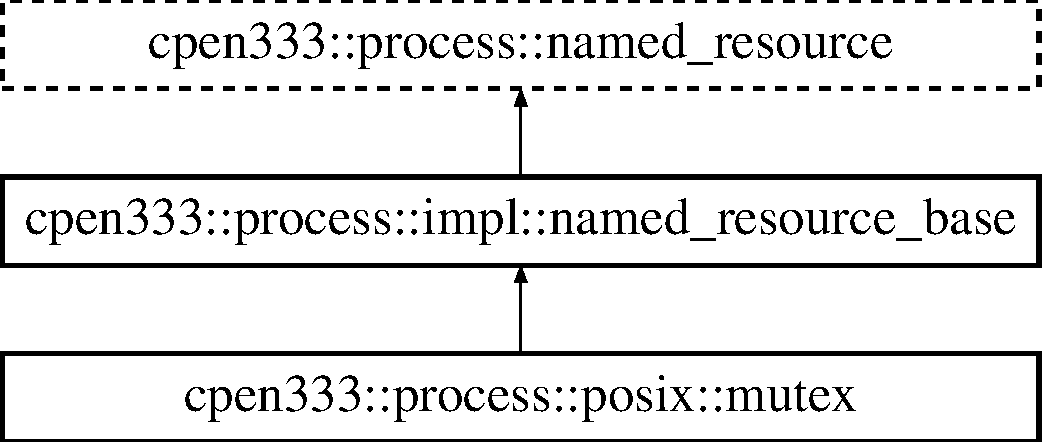
\includegraphics[height=3.000000cm]{classcpen333_1_1process_1_1posix_1_1mutex}
\end{center}
\end{figure}
\subsection*{Public Types}
\begin{DoxyCompactItemize}
\item 
\mbox{\Hypertarget{classcpen333_1_1process_1_1posix_1_1mutex_aac6d3675fcffc52ddf281e952968e44b}\label{classcpen333_1_1process_1_1posix_1_1mutex_aac6d3675fcffc52ddf281e952968e44b}} 
using \hyperlink{classcpen333_1_1process_1_1posix_1_1mutex_aac6d3675fcffc52ddf281e952968e44b}{native\+\_\+handle\+\_\+type} = \hyperlink{classcpen333_1_1process_1_1posix_1_1semaphore_ad63150e5c8c196a84a7b214462756f1a}{semaphore\+::native\+\_\+handle\+\_\+type}
\begin{DoxyCompactList}\small\item\em Alias to the underlying native mutex handle. \end{DoxyCompactList}\end{DoxyCompactItemize}
\subsection*{Public Member Functions}
\begin{DoxyCompactItemize}
\item 
\hyperlink{classcpen333_1_1process_1_1posix_1_1mutex_a72ecaf79b2e4ea585b542dc0ed240614}{mutex} (const std\+::string \&\hyperlink{classcpen333_1_1process_1_1impl_1_1named__resource__base_a53986a0a1dd26a3602b842c45613b79d}{name})
\begin{DoxyCompactList}\small\item\em Constructs or connects to the named mutex. \end{DoxyCompactList}\item 
void \hyperlink{classcpen333_1_1process_1_1posix_1_1mutex_a07dccda80dc88292fa490ce47dd0faa6}{lock} ()
\begin{DoxyCompactList}\small\item\em Locks the mutex. \end{DoxyCompactList}\item 
bool \hyperlink{classcpen333_1_1process_1_1posix_1_1mutex_ae19f7c8370308f7333cee340fef91049}{try\+\_\+lock} ()
\begin{DoxyCompactList}\small\item\em Tries to lock the mutex. \end{DoxyCompactList}\item 
{\footnotesize template$<$class Rep , class Period $>$ }\\bool \hyperlink{classcpen333_1_1process_1_1posix_1_1mutex_a28ac1db650efaae2d959df0e555f3d24}{try\+\_\+lock\+\_\+for} (const std\+::chrono\+::duration$<$ Rep, Period $>$ \&timeout\+\_\+duration)
\begin{DoxyCompactList}\small\item\em Tries to lock the mutex until a relative time has elapsed. \end{DoxyCompactList}\item 
{\footnotesize template$<$class Clock , class Duration $>$ }\\bool \hyperlink{classcpen333_1_1process_1_1posix_1_1mutex_a0cfd76098d89d269ad4a89115e7673d1}{try\+\_\+lock\+\_\+until} (const std\+::chrono\+::time\+\_\+point$<$ Clock, Duration $>$ \&timeout\+\_\+time)
\begin{DoxyCompactList}\small\item\em Tries to lock the mutex until an absolute time has passed. \end{DoxyCompactList}\item 
void \hyperlink{classcpen333_1_1process_1_1posix_1_1mutex_a822e51a57ea9e5de1a052aeddf3e4e02}{unlock} ()
\begin{DoxyCompactList}\small\item\em Unlocks the mutex. \end{DoxyCompactList}\item 
\hyperlink{classcpen333_1_1process_1_1posix_1_1mutex_aac6d3675fcffc52ddf281e952968e44b}{native\+\_\+handle\+\_\+type} \hyperlink{classcpen333_1_1process_1_1posix_1_1mutex_aa36462cbd2181e20caa35656c619c6dd}{native\+\_\+handle} ()
\begin{DoxyCompactList}\small\item\em Returns a native handle. \end{DoxyCompactList}\item 
bool \hyperlink{classcpen333_1_1process_1_1posix_1_1mutex_ac1bcf9576d7470e5d64e17876c9cdb36}{unlink} ()
\begin{DoxyCompactList}\small\item\em Detaches the name from the named resource. \end{DoxyCompactList}\end{DoxyCompactItemize}
\subsection*{Static Public Member Functions}
\begin{DoxyCompactItemize}
\item 
static bool \hyperlink{classcpen333_1_1process_1_1posix_1_1mutex_ae5750c148e0408daac498a87d2d9a579}{unlink} (const std\+::string \&\hyperlink{classcpen333_1_1process_1_1impl_1_1named__resource__base_a53986a0a1dd26a3602b842c45613b79d}{name})
\begin{DoxyCompactList}\small\item\em Unlinks the name without needing to create a resource. \end{DoxyCompactList}\end{DoxyCompactItemize}
\subsection*{Additional Inherited Members}


\subsection{Detailed Description}
Inter-\/process named mutual exclusion primitive. 

Used to limit resource access to one thread at a time

Based on a named semaphore. Unlike a true mutex, this implementation does N\+OT enforce that the same thread unlock the mutex. However, in practice, it should be treated as a true mutex by using std\+::lock\+\_\+guard or std\+::unique\+\_\+lock.

This mutex has K\+E\+R\+N\+EL P\+E\+R\+S\+I\+S\+T\+E\+N\+CE, meaning if not \hyperlink{classcpen333_1_1process_1_1posix_1_1mutex_ac1bcf9576d7470e5d64e17876c9cdb36}{unlink()}-\/ed, will continue to exist in its current state until the system is shut down (persisting beyond the life of the initiating program) 

\subsection{Constructor \& Destructor Documentation}
\mbox{\Hypertarget{classcpen333_1_1process_1_1posix_1_1mutex_a72ecaf79b2e4ea585b542dc0ed240614}\label{classcpen333_1_1process_1_1posix_1_1mutex_a72ecaf79b2e4ea585b542dc0ed240614}} 
\index{cpen333\+::process\+::posix\+::mutex@{cpen333\+::process\+::posix\+::mutex}!mutex@{mutex}}
\index{mutex@{mutex}!cpen333\+::process\+::posix\+::mutex@{cpen333\+::process\+::posix\+::mutex}}
\subsubsection{\texorpdfstring{mutex()}{mutex()}}
{\footnotesize\ttfamily cpen333\+::process\+::posix\+::mutex\+::mutex (\begin{DoxyParamCaption}\item[{const std\+::string \&}]{name }\end{DoxyParamCaption})\hspace{0.3cm}{\ttfamily [inline]}}



Constructs or connects to the named mutex. 


\begin{DoxyParams}{Parameters}
{\em name} & identifier for creating or connecting to an existing inter-\/process mutex \\
\hline
\end{DoxyParams}


\subsection{Member Function Documentation}
\mbox{\Hypertarget{classcpen333_1_1process_1_1posix_1_1mutex_a07dccda80dc88292fa490ce47dd0faa6}\label{classcpen333_1_1process_1_1posix_1_1mutex_a07dccda80dc88292fa490ce47dd0faa6}} 
\index{cpen333\+::process\+::posix\+::mutex@{cpen333\+::process\+::posix\+::mutex}!lock@{lock}}
\index{lock@{lock}!cpen333\+::process\+::posix\+::mutex@{cpen333\+::process\+::posix\+::mutex}}
\subsubsection{\texorpdfstring{lock()}{lock()}}
{\footnotesize\ttfamily void cpen333\+::process\+::posix\+::mutex\+::lock (\begin{DoxyParamCaption}{ }\end{DoxyParamCaption})\hspace{0.3cm}{\ttfamily [inline]}}



Locks the mutex. 

This will block the current thread until the mutex is available to be locked, preventing multiple threads from accessing a protected resource. \mbox{\Hypertarget{classcpen333_1_1process_1_1posix_1_1mutex_aa36462cbd2181e20caa35656c619c6dd}\label{classcpen333_1_1process_1_1posix_1_1mutex_aa36462cbd2181e20caa35656c619c6dd}} 
\index{cpen333\+::process\+::posix\+::mutex@{cpen333\+::process\+::posix\+::mutex}!native\+\_\+handle@{native\+\_\+handle}}
\index{native\+\_\+handle@{native\+\_\+handle}!cpen333\+::process\+::posix\+::mutex@{cpen333\+::process\+::posix\+::mutex}}
\subsubsection{\texorpdfstring{native\+\_\+handle()}{native\_handle()}}
{\footnotesize\ttfamily \hyperlink{classcpen333_1_1process_1_1posix_1_1mutex_aac6d3675fcffc52ddf281e952968e44b}{native\+\_\+handle\+\_\+type} cpen333\+::process\+::posix\+::mutex\+::native\+\_\+handle (\begin{DoxyParamCaption}{ }\end{DoxyParamCaption})\hspace{0.3cm}{\ttfamily [inline]}}



Returns a native handle. 

In this case, a P\+O\+S\+IX sem\+\_\+t

\begin{DoxyReturn}{Returns}
native handle to underlying mutex 
\end{DoxyReturn}
\mbox{\Hypertarget{classcpen333_1_1process_1_1posix_1_1mutex_ae19f7c8370308f7333cee340fef91049}\label{classcpen333_1_1process_1_1posix_1_1mutex_ae19f7c8370308f7333cee340fef91049}} 
\index{cpen333\+::process\+::posix\+::mutex@{cpen333\+::process\+::posix\+::mutex}!try\+\_\+lock@{try\+\_\+lock}}
\index{try\+\_\+lock@{try\+\_\+lock}!cpen333\+::process\+::posix\+::mutex@{cpen333\+::process\+::posix\+::mutex}}
\subsubsection{\texorpdfstring{try\+\_\+lock()}{try\_lock()}}
{\footnotesize\ttfamily bool cpen333\+::process\+::posix\+::mutex\+::try\+\_\+lock (\begin{DoxyParamCaption}{ }\end{DoxyParamCaption})\hspace{0.3cm}{\ttfamily [inline]}}



Tries to lock the mutex. 

This will attempt to lock the mutex, returning immediately.

\begin{DoxyReturn}{Returns}
true if locked successfully, false if already locked 
\end{DoxyReturn}
\mbox{\Hypertarget{classcpen333_1_1process_1_1posix_1_1mutex_a28ac1db650efaae2d959df0e555f3d24}\label{classcpen333_1_1process_1_1posix_1_1mutex_a28ac1db650efaae2d959df0e555f3d24}} 
\index{cpen333\+::process\+::posix\+::mutex@{cpen333\+::process\+::posix\+::mutex}!try\+\_\+lock\+\_\+for@{try\+\_\+lock\+\_\+for}}
\index{try\+\_\+lock\+\_\+for@{try\+\_\+lock\+\_\+for}!cpen333\+::process\+::posix\+::mutex@{cpen333\+::process\+::posix\+::mutex}}
\subsubsection{\texorpdfstring{try\+\_\+lock\+\_\+for()}{try\_lock\_for()}}
{\footnotesize\ttfamily template$<$class Rep , class Period $>$ \\
bool cpen333\+::process\+::posix\+::mutex\+::try\+\_\+lock\+\_\+for (\begin{DoxyParamCaption}\item[{const std\+::chrono\+::duration$<$ Rep, Period $>$ \&}]{timeout\+\_\+duration }\end{DoxyParamCaption})\hspace{0.3cm}{\ttfamily [inline]}}



Tries to lock the mutex until a relative time has elapsed. 

Blocks until the specified timeout duration has elapsed or the lock is acquired, whichever comes first.


\begin{DoxyTemplParams}{Template Parameters}
{\em Rep} & timer representation \\
\hline
{\em Period} & timeout period type \\
\hline
\end{DoxyTemplParams}

\begin{DoxyParams}{Parameters}
{\em timeout\+\_\+duration} & maximum relative time to block for \\
\hline
\end{DoxyParams}
\begin{DoxyReturn}{Returns}
true if lock was acquired successfully, false otherwise 
\end{DoxyReturn}
\mbox{\Hypertarget{classcpen333_1_1process_1_1posix_1_1mutex_a0cfd76098d89d269ad4a89115e7673d1}\label{classcpen333_1_1process_1_1posix_1_1mutex_a0cfd76098d89d269ad4a89115e7673d1}} 
\index{cpen333\+::process\+::posix\+::mutex@{cpen333\+::process\+::posix\+::mutex}!try\+\_\+lock\+\_\+until@{try\+\_\+lock\+\_\+until}}
\index{try\+\_\+lock\+\_\+until@{try\+\_\+lock\+\_\+until}!cpen333\+::process\+::posix\+::mutex@{cpen333\+::process\+::posix\+::mutex}}
\subsubsection{\texorpdfstring{try\+\_\+lock\+\_\+until()}{try\_lock\_until()}}
{\footnotesize\ttfamily template$<$class Clock , class Duration $>$ \\
bool cpen333\+::process\+::posix\+::mutex\+::try\+\_\+lock\+\_\+until (\begin{DoxyParamCaption}\item[{const std\+::chrono\+::time\+\_\+point$<$ Clock, Duration $>$ \&}]{timeout\+\_\+time }\end{DoxyParamCaption})\hspace{0.3cm}{\ttfamily [inline]}}



Tries to lock the mutex until an absolute time has passed. 


\begin{DoxyTemplParams}{Template Parameters}
{\em Clock} & timeout clock type \\
\hline
{\em Duration} & timeout duration type \\
\hline
\end{DoxyTemplParams}

\begin{DoxyParams}{Parameters}
{\em timeout\+\_\+time} & absolute timeout time \\
\hline
\end{DoxyParams}
\begin{DoxyReturn}{Returns}
true if the lock was acquired successfully, false otherwise 
\end{DoxyReturn}
\mbox{\Hypertarget{classcpen333_1_1process_1_1posix_1_1mutex_ac1bcf9576d7470e5d64e17876c9cdb36}\label{classcpen333_1_1process_1_1posix_1_1mutex_ac1bcf9576d7470e5d64e17876c9cdb36}} 
\index{cpen333\+::process\+::posix\+::mutex@{cpen333\+::process\+::posix\+::mutex}!unlink@{unlink}}
\index{unlink@{unlink}!cpen333\+::process\+::posix\+::mutex@{cpen333\+::process\+::posix\+::mutex}}
\subsubsection{\texorpdfstring{unlink()}{unlink()}\hspace{0.1cm}{\footnotesize\ttfamily [1/2]}}
{\footnotesize\ttfamily bool cpen333\+::process\+::posix\+::mutex\+::unlink (\begin{DoxyParamCaption}{ }\end{DoxyParamCaption})\hspace{0.3cm}{\ttfamily [inline]}, {\ttfamily [virtual]}}



Detaches the name from the named resource. 

On P\+O\+S\+IX systems, named resources will persist beyond the lifetime of any process that uses them as long as the name has not been unlinked (or until the system is rebooted). Calling {\ttfamily unlink} will detach the name, allowing the resource to be freed once all current users have exited.

\begin{DoxyReturn}{Returns}
{\ttfamily true} if unlink is successful, {\ttfamily false} if unlinking is not supported or if an error has occurred. 
\end{DoxyReturn}


Implements \hyperlink{classcpen333_1_1process_1_1impl_1_1named__resource__base_ae4033f82dfd068b917a9bca57d3a0c45}{cpen333\+::process\+::impl\+::named\+\_\+resource\+\_\+base}.

\mbox{\Hypertarget{classcpen333_1_1process_1_1posix_1_1mutex_ae5750c148e0408daac498a87d2d9a579}\label{classcpen333_1_1process_1_1posix_1_1mutex_ae5750c148e0408daac498a87d2d9a579}} 
\index{cpen333\+::process\+::posix\+::mutex@{cpen333\+::process\+::posix\+::mutex}!unlink@{unlink}}
\index{unlink@{unlink}!cpen333\+::process\+::posix\+::mutex@{cpen333\+::process\+::posix\+::mutex}}
\subsubsection{\texorpdfstring{unlink()}{unlink()}\hspace{0.1cm}{\footnotesize\ttfamily [2/2]}}
{\footnotesize\ttfamily static bool cpen333\+::process\+::posix\+::mutex\+::unlink (\begin{DoxyParamCaption}\item[{const std\+::string \&}]{name }\end{DoxyParamCaption})\hspace{0.3cm}{\ttfamily [inline]}, {\ttfamily [static]}}



Unlinks the name without needing to create a resource. 

Implementers should also provide a static method for unlinking. The purpose is mainly for clean-\/up of existing resources.


\begin{DoxyParams}{Parameters}
{\em name} & desired resource name \\
\hline
\end{DoxyParams}
\begin{DoxyReturn}{Returns}
{\ttfamily true} if unlink successful, {\ttfamily false} if not successful or not supported 
\end{DoxyReturn}
\mbox{\Hypertarget{classcpen333_1_1process_1_1posix_1_1mutex_a822e51a57ea9e5de1a052aeddf3e4e02}\label{classcpen333_1_1process_1_1posix_1_1mutex_a822e51a57ea9e5de1a052aeddf3e4e02}} 
\index{cpen333\+::process\+::posix\+::mutex@{cpen333\+::process\+::posix\+::mutex}!unlock@{unlock}}
\index{unlock@{unlock}!cpen333\+::process\+::posix\+::mutex@{cpen333\+::process\+::posix\+::mutex}}
\subsubsection{\texorpdfstring{unlock()}{unlock()}}
{\footnotesize\ttfamily void cpen333\+::process\+::posix\+::mutex\+::unlock (\begin{DoxyParamCaption}{ }\end{DoxyParamCaption})\hspace{0.3cm}{\ttfamily [inline]}}



Unlocks the mutex. 

Puts the mutex in a state to be relocked, freeing the protected resource to be used by another (or the same) thread 

The documentation for this class was generated from the following file\+:\begin{DoxyCompactItemize}
\item 
D\+:/school/teaching/\+C\+P\+E\+N333/workspace/library/include/cpen333/process/impl/posix/\hyperlink{impl_2posix_2mutex_8h}{mutex.\+h}\end{DoxyCompactItemize}

\hypertarget{classcpen333_1_1process_1_1windows_1_1mutex}{}\section{cpen333\+:\+:process\+:\+:windows\+:\+:mutex Class Reference}
\label{classcpen333_1_1process_1_1windows_1_1mutex}\index{cpen333\+::process\+::windows\+::mutex@{cpen333\+::process\+::windows\+::mutex}}


Inter-\/process named mutual exclusion primitive.  




{\ttfamily \#include $<$mutex.\+h$>$}

Inheritance diagram for cpen333\+:\+:process\+:\+:windows\+:\+:mutex\+:\begin{figure}[H]
\begin{center}
\leavevmode
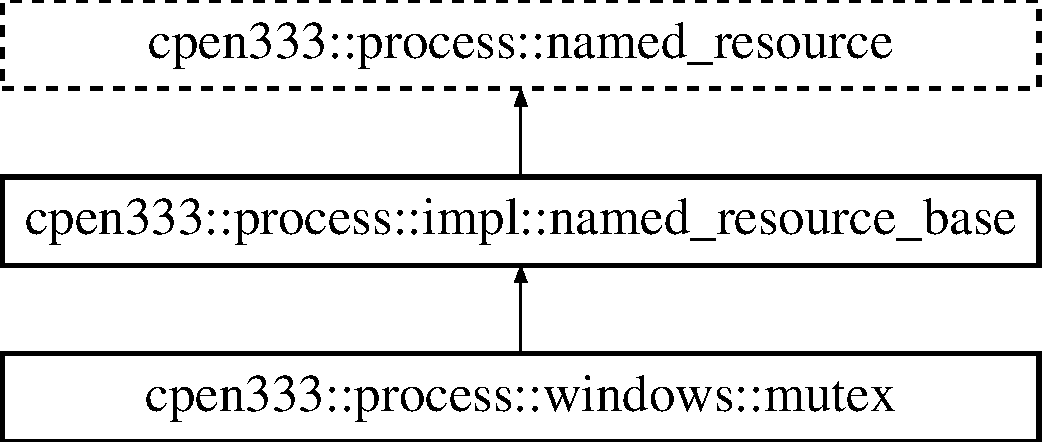
\includegraphics[height=3.000000cm]{classcpen333_1_1process_1_1windows_1_1mutex}
\end{center}
\end{figure}
\subsection*{Public Types}
\begin{DoxyCompactItemize}
\item 
\mbox{\Hypertarget{classcpen333_1_1process_1_1windows_1_1mutex_ae2343808c470604a4291106bfad2ca50}\label{classcpen333_1_1process_1_1windows_1_1mutex_ae2343808c470604a4291106bfad2ca50}} 
typedef H\+A\+N\+D\+LE \hyperlink{classcpen333_1_1process_1_1windows_1_1mutex_ae2343808c470604a4291106bfad2ca50}{native\+\_\+handle\+\_\+type}
\begin{DoxyCompactList}\small\item\em Alias to native handle type, which on Windows is type H\+A\+N\+D\+LE. \end{DoxyCompactList}\end{DoxyCompactItemize}
\subsection*{Public Member Functions}
\begin{DoxyCompactItemize}
\item 
\hyperlink{classcpen333_1_1process_1_1windows_1_1mutex_a6bd2d0c07f83dd5646cbdbadbfc8fc58}{mutex} (const std\+::string \&\hyperlink{classcpen333_1_1process_1_1impl_1_1named__resource__base_a53986a0a1dd26a3602b842c45613b79d}{name})
\begin{DoxyCompactList}\small\item\em Constructs or connects to the named mutex. \end{DoxyCompactList}\item 
\mbox{\Hypertarget{classcpen333_1_1process_1_1windows_1_1mutex_a51a169fed979fd4dcb0a4f9c17cdb99e}\label{classcpen333_1_1process_1_1windows_1_1mutex_a51a169fed979fd4dcb0a4f9c17cdb99e}} 
\hyperlink{classcpen333_1_1process_1_1windows_1_1mutex_a51a169fed979fd4dcb0a4f9c17cdb99e}{$\sim$mutex} ()
\begin{DoxyCompactList}\small\item\em Destructor, closes this instance\textquotesingle{}s handle to the shared mutex. \end{DoxyCompactList}\item 
void \hyperlink{classcpen333_1_1process_1_1windows_1_1mutex_a887f0647207b0e0fa1bead1500c95aec}{lock} ()
\begin{DoxyCompactList}\small\item\em Locks the mutex. \end{DoxyCompactList}\item 
bool \hyperlink{classcpen333_1_1process_1_1windows_1_1mutex_a8fe777a1d576868de91b34d3727132e2}{try\+\_\+lock} ()
\begin{DoxyCompactList}\small\item\em Tries to lock the mutex. \end{DoxyCompactList}\item 
{\footnotesize template$<$class Rep , class Period $>$ }\\bool \hyperlink{classcpen333_1_1process_1_1windows_1_1mutex_aa6a64c60b601c226648cce293835c802}{try\+\_\+lock\+\_\+for} (const std\+::chrono\+::duration$<$ Rep, Period $>$ \&timeout\+\_\+duration)
\begin{DoxyCompactList}\small\item\em Tries to lock the mutex until a relative time has elapsed. \end{DoxyCompactList}\item 
{\footnotesize template$<$class Clock , class Duration $>$ }\\bool \hyperlink{classcpen333_1_1process_1_1windows_1_1mutex_a87d22d9dce4211d0e077cbf7db462fdf}{try\+\_\+lock\+\_\+until} (const std\+::chrono\+::time\+\_\+point$<$ Clock, Duration $>$ \&timeout\+\_\+time)
\begin{DoxyCompactList}\small\item\em Tries to lock the mutex until an absolute time has passed. \end{DoxyCompactList}\item 
bool \hyperlink{classcpen333_1_1process_1_1windows_1_1mutex_a998f0f3d2e56d3acf63a30b465e153a7}{unlock} ()
\begin{DoxyCompactList}\small\item\em Unlocks the mutex. \end{DoxyCompactList}\item 
\hyperlink{classcpen333_1_1process_1_1windows_1_1mutex_ae2343808c470604a4291106bfad2ca50}{native\+\_\+handle\+\_\+type} \hyperlink{classcpen333_1_1process_1_1windows_1_1mutex_a44a60d5a4d372684c8278e7a1f952fb6}{native\+\_\+handle} ()
\begin{DoxyCompactList}\small\item\em Returns a native handle. \end{DoxyCompactList}\item 
bool \hyperlink{classcpen333_1_1process_1_1windows_1_1mutex_aa45381a0a226fbefc86eef8971a5431b}{unlink} ()
\begin{DoxyCompactList}\small\item\em Detaches the name from the named resource. \end{DoxyCompactList}\end{DoxyCompactItemize}
\subsection*{Static Public Member Functions}
\begin{DoxyCompactItemize}
\item 
static bool \hyperlink{classcpen333_1_1process_1_1windows_1_1mutex_aa5a57e9c9c3fdb82bc69c8d1c68ddbfd}{unlink} (const std\+::string \&\hyperlink{classcpen333_1_1process_1_1impl_1_1named__resource__base_a53986a0a1dd26a3602b842c45613b79d}{name})
\begin{DoxyCompactList}\small\item\em Unlinks the name without needing to create a resource. \end{DoxyCompactList}\end{DoxyCompactItemize}
\subsection*{Additional Inherited Members}


\subsection{Detailed Description}
Inter-\/process named mutual exclusion primitive. 

Used to limit resource access to one thread at a time

This mutex has U\+S\+A\+GE P\+E\+R\+S\+I\+S\+T\+E\+N\+CE, meaning the mutex will continue to exist as long as at least one process/thread is holding a reference to it. 

\subsection{Constructor \& Destructor Documentation}
\mbox{\Hypertarget{classcpen333_1_1process_1_1windows_1_1mutex_a6bd2d0c07f83dd5646cbdbadbfc8fc58}\label{classcpen333_1_1process_1_1windows_1_1mutex_a6bd2d0c07f83dd5646cbdbadbfc8fc58}} 
\index{cpen333\+::process\+::windows\+::mutex@{cpen333\+::process\+::windows\+::mutex}!mutex@{mutex}}
\index{mutex@{mutex}!cpen333\+::process\+::windows\+::mutex@{cpen333\+::process\+::windows\+::mutex}}
\subsubsection{\texorpdfstring{mutex()}{mutex()}}
{\footnotesize\ttfamily cpen333\+::process\+::windows\+::mutex\+::mutex (\begin{DoxyParamCaption}\item[{const std\+::string \&}]{name }\end{DoxyParamCaption})\hspace{0.3cm}{\ttfamily [inline]}}



Constructs or connects to the named mutex. 


\begin{DoxyParams}{Parameters}
{\em name} & identifier for creating or connecting to an existing inter-\/process mutex \\
\hline
\end{DoxyParams}


\subsection{Member Function Documentation}
\mbox{\Hypertarget{classcpen333_1_1process_1_1windows_1_1mutex_a887f0647207b0e0fa1bead1500c95aec}\label{classcpen333_1_1process_1_1windows_1_1mutex_a887f0647207b0e0fa1bead1500c95aec}} 
\index{cpen333\+::process\+::windows\+::mutex@{cpen333\+::process\+::windows\+::mutex}!lock@{lock}}
\index{lock@{lock}!cpen333\+::process\+::windows\+::mutex@{cpen333\+::process\+::windows\+::mutex}}
\subsubsection{\texorpdfstring{lock()}{lock()}}
{\footnotesize\ttfamily void cpen333\+::process\+::windows\+::mutex\+::lock (\begin{DoxyParamCaption}{ }\end{DoxyParamCaption})\hspace{0.3cm}{\ttfamily [inline]}}



Locks the mutex. 

This will block the current thread until the mutex is available to be locked, preventing multiple threads from accessing a protected resource. \mbox{\Hypertarget{classcpen333_1_1process_1_1windows_1_1mutex_a44a60d5a4d372684c8278e7a1f952fb6}\label{classcpen333_1_1process_1_1windows_1_1mutex_a44a60d5a4d372684c8278e7a1f952fb6}} 
\index{cpen333\+::process\+::windows\+::mutex@{cpen333\+::process\+::windows\+::mutex}!native\+\_\+handle@{native\+\_\+handle}}
\index{native\+\_\+handle@{native\+\_\+handle}!cpen333\+::process\+::windows\+::mutex@{cpen333\+::process\+::windows\+::mutex}}
\subsubsection{\texorpdfstring{native\+\_\+handle()}{native\_handle()}}
{\footnotesize\ttfamily \hyperlink{classcpen333_1_1process_1_1windows_1_1mutex_ae2343808c470604a4291106bfad2ca50}{native\+\_\+handle\+\_\+type} cpen333\+::process\+::windows\+::mutex\+::native\+\_\+handle (\begin{DoxyParamCaption}{ }\end{DoxyParamCaption})\hspace{0.3cm}{\ttfamily [inline]}}



Returns a native handle. 

In this case, a Windows H\+A\+N\+D\+LE to the Mutex

\begin{DoxyReturn}{Returns}
native handle to underlying mutex 
\end{DoxyReturn}
\mbox{\Hypertarget{classcpen333_1_1process_1_1windows_1_1mutex_a8fe777a1d576868de91b34d3727132e2}\label{classcpen333_1_1process_1_1windows_1_1mutex_a8fe777a1d576868de91b34d3727132e2}} 
\index{cpen333\+::process\+::windows\+::mutex@{cpen333\+::process\+::windows\+::mutex}!try\+\_\+lock@{try\+\_\+lock}}
\index{try\+\_\+lock@{try\+\_\+lock}!cpen333\+::process\+::windows\+::mutex@{cpen333\+::process\+::windows\+::mutex}}
\subsubsection{\texorpdfstring{try\+\_\+lock()}{try\_lock()}}
{\footnotesize\ttfamily bool cpen333\+::process\+::windows\+::mutex\+::try\+\_\+lock (\begin{DoxyParamCaption}{ }\end{DoxyParamCaption})\hspace{0.3cm}{\ttfamily [inline]}}



Tries to lock the mutex. 

This will attempt to lock the mutex, returning immediately.

\begin{DoxyReturn}{Returns}
true if locked successfully, false if already locked 
\end{DoxyReturn}
\mbox{\Hypertarget{classcpen333_1_1process_1_1windows_1_1mutex_aa6a64c60b601c226648cce293835c802}\label{classcpen333_1_1process_1_1windows_1_1mutex_aa6a64c60b601c226648cce293835c802}} 
\index{cpen333\+::process\+::windows\+::mutex@{cpen333\+::process\+::windows\+::mutex}!try\+\_\+lock\+\_\+for@{try\+\_\+lock\+\_\+for}}
\index{try\+\_\+lock\+\_\+for@{try\+\_\+lock\+\_\+for}!cpen333\+::process\+::windows\+::mutex@{cpen333\+::process\+::windows\+::mutex}}
\subsubsection{\texorpdfstring{try\+\_\+lock\+\_\+for()}{try\_lock\_for()}}
{\footnotesize\ttfamily template$<$class Rep , class Period $>$ \\
bool cpen333\+::process\+::windows\+::mutex\+::try\+\_\+lock\+\_\+for (\begin{DoxyParamCaption}\item[{const std\+::chrono\+::duration$<$ Rep, Period $>$ \&}]{timeout\+\_\+duration }\end{DoxyParamCaption})\hspace{0.3cm}{\ttfamily [inline]}}



Tries to lock the mutex until a relative time has elapsed. 

Blocks until the specified timeout duration has elapsed or the lock is acquired, whichever comes first.


\begin{DoxyTemplParams}{Template Parameters}
{\em Rep} & timer representation \\
\hline
{\em Period} & timeout period type \\
\hline
\end{DoxyTemplParams}

\begin{DoxyParams}{Parameters}
{\em timeout\+\_\+duration} & maximum relative time to block for \\
\hline
\end{DoxyParams}
\begin{DoxyReturn}{Returns}
true if lock was acquired successfully, false otherwise 
\end{DoxyReturn}
\mbox{\Hypertarget{classcpen333_1_1process_1_1windows_1_1mutex_a87d22d9dce4211d0e077cbf7db462fdf}\label{classcpen333_1_1process_1_1windows_1_1mutex_a87d22d9dce4211d0e077cbf7db462fdf}} 
\index{cpen333\+::process\+::windows\+::mutex@{cpen333\+::process\+::windows\+::mutex}!try\+\_\+lock\+\_\+until@{try\+\_\+lock\+\_\+until}}
\index{try\+\_\+lock\+\_\+until@{try\+\_\+lock\+\_\+until}!cpen333\+::process\+::windows\+::mutex@{cpen333\+::process\+::windows\+::mutex}}
\subsubsection{\texorpdfstring{try\+\_\+lock\+\_\+until()}{try\_lock\_until()}}
{\footnotesize\ttfamily template$<$class Clock , class Duration $>$ \\
bool cpen333\+::process\+::windows\+::mutex\+::try\+\_\+lock\+\_\+until (\begin{DoxyParamCaption}\item[{const std\+::chrono\+::time\+\_\+point$<$ Clock, Duration $>$ \&}]{timeout\+\_\+time }\end{DoxyParamCaption})\hspace{0.3cm}{\ttfamily [inline]}}



Tries to lock the mutex until an absolute time has passed. 


\begin{DoxyTemplParams}{Template Parameters}
{\em Clock} & timeout clock type \\
\hline
{\em Duration} & timeout duration type \\
\hline
\end{DoxyTemplParams}

\begin{DoxyParams}{Parameters}
{\em timeout\+\_\+time} & absolute timeout time \\
\hline
\end{DoxyParams}
\begin{DoxyReturn}{Returns}
true if the lock was acquired successfully, false otherwise 
\end{DoxyReturn}
\mbox{\Hypertarget{classcpen333_1_1process_1_1windows_1_1mutex_aa45381a0a226fbefc86eef8971a5431b}\label{classcpen333_1_1process_1_1windows_1_1mutex_aa45381a0a226fbefc86eef8971a5431b}} 
\index{cpen333\+::process\+::windows\+::mutex@{cpen333\+::process\+::windows\+::mutex}!unlink@{unlink}}
\index{unlink@{unlink}!cpen333\+::process\+::windows\+::mutex@{cpen333\+::process\+::windows\+::mutex}}
\subsubsection{\texorpdfstring{unlink()}{unlink()}\hspace{0.1cm}{\footnotesize\ttfamily [1/2]}}
{\footnotesize\ttfamily bool cpen333\+::process\+::windows\+::mutex\+::unlink (\begin{DoxyParamCaption}{ }\end{DoxyParamCaption})\hspace{0.3cm}{\ttfamily [inline]}, {\ttfamily [virtual]}}



Detaches the name from the named resource. 

On P\+O\+S\+IX systems, named resources will persist beyond the lifetime of any process that uses them as long as the name has not been unlinked (or until the system is rebooted). Calling {\ttfamily unlink} will detach the name, allowing the resource to be freed once all current users have exited.

\begin{DoxyReturn}{Returns}
{\ttfamily true} if unlink is successful, {\ttfamily false} if unlinking is not supported or if an error has occurred. 
\end{DoxyReturn}


Implements \hyperlink{classcpen333_1_1process_1_1impl_1_1named__resource__base_ae4033f82dfd068b917a9bca57d3a0c45}{cpen333\+::process\+::impl\+::named\+\_\+resource\+\_\+base}.

\mbox{\Hypertarget{classcpen333_1_1process_1_1windows_1_1mutex_aa5a57e9c9c3fdb82bc69c8d1c68ddbfd}\label{classcpen333_1_1process_1_1windows_1_1mutex_aa5a57e9c9c3fdb82bc69c8d1c68ddbfd}} 
\index{cpen333\+::process\+::windows\+::mutex@{cpen333\+::process\+::windows\+::mutex}!unlink@{unlink}}
\index{unlink@{unlink}!cpen333\+::process\+::windows\+::mutex@{cpen333\+::process\+::windows\+::mutex}}
\subsubsection{\texorpdfstring{unlink()}{unlink()}\hspace{0.1cm}{\footnotesize\ttfamily [2/2]}}
{\footnotesize\ttfamily static bool cpen333\+::process\+::windows\+::mutex\+::unlink (\begin{DoxyParamCaption}\item[{const std\+::string \&}]{name }\end{DoxyParamCaption})\hspace{0.3cm}{\ttfamily [inline]}, {\ttfamily [static]}}



Unlinks the name without needing to create a resource. 

Implementers should also provide a static method for unlinking. The purpose is mainly for clean-\/up of existing resources.


\begin{DoxyParams}{Parameters}
{\em name} & desired resource name \\
\hline
\end{DoxyParams}
\begin{DoxyReturn}{Returns}
{\ttfamily true} if unlink successful, {\ttfamily false} if not successful or not supported 
\end{DoxyReturn}
\mbox{\Hypertarget{classcpen333_1_1process_1_1windows_1_1mutex_a998f0f3d2e56d3acf63a30b465e153a7}\label{classcpen333_1_1process_1_1windows_1_1mutex_a998f0f3d2e56d3acf63a30b465e153a7}} 
\index{cpen333\+::process\+::windows\+::mutex@{cpen333\+::process\+::windows\+::mutex}!unlock@{unlock}}
\index{unlock@{unlock}!cpen333\+::process\+::windows\+::mutex@{cpen333\+::process\+::windows\+::mutex}}
\subsubsection{\texorpdfstring{unlock()}{unlock()}}
{\footnotesize\ttfamily bool cpen333\+::process\+::windows\+::mutex\+::unlock (\begin{DoxyParamCaption}{ }\end{DoxyParamCaption})\hspace{0.3cm}{\ttfamily [inline]}}



Unlocks the mutex. 

Puts the mutex in a state to be relocked, freeing the protected resource to be used by another (or the same) thread 

The documentation for this class was generated from the following file\+:\begin{DoxyCompactItemize}
\item 
D\+:/school/teaching/\+C\+P\+E\+N333/workspace/library/include/cpen333/process/impl/windows/\hyperlink{impl_2windows_2mutex_8h}{mutex.\+h}\end{DoxyCompactItemize}

\input{classcpen333_1_1process_1_1mutex}
\hypertarget{classcpen333_1_1process_1_1named__resource}{}\section{cpen333\+:\+:process\+:\+:named\+\_\+resource Class Reference}
\label{classcpen333_1_1process_1_1named__resource}\index{cpen333\+::process\+::named\+\_\+resource@{cpen333\+::process\+::named\+\_\+resource}}


Pure virtual base class for all inter-\/process resources.  




{\ttfamily \#include $<$named\+\_\+resource.\+h$>$}

Inheritance diagram for cpen333\+:\+:process\+:\+:named\+\_\+resource\+:\begin{figure}[H]
\begin{center}
\leavevmode
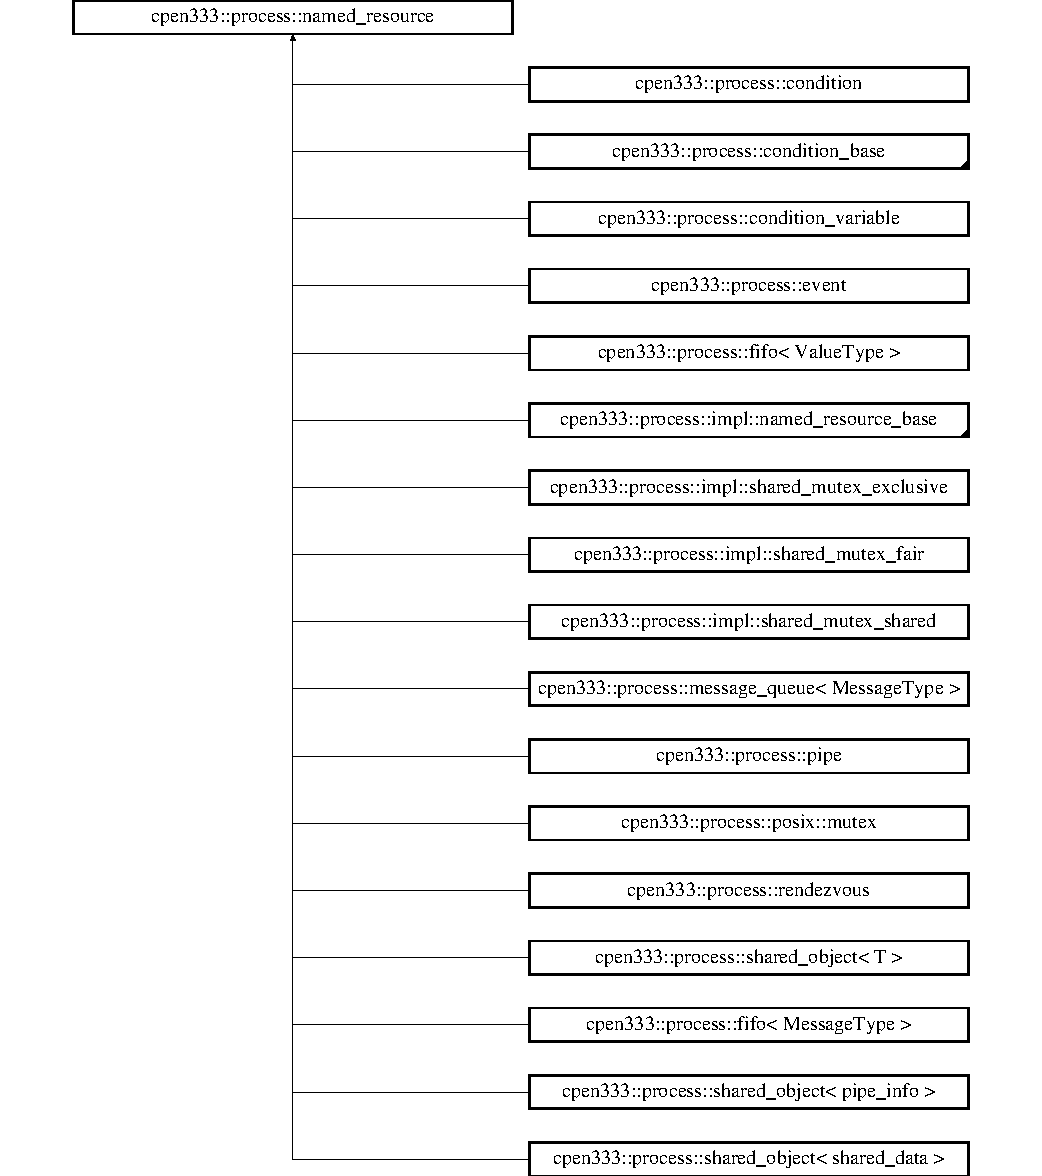
\includegraphics[height=12.000000cm]{classcpen333_1_1process_1_1named__resource}
\end{center}
\end{figure}
\subsection*{Public Member Functions}
\begin{DoxyCompactItemize}
\item 
\mbox{\Hypertarget{classcpen333_1_1process_1_1named__resource_a2bf88d9fa295c5e9ffecf2a43414e6da}\label{classcpen333_1_1process_1_1named__resource_a2bf88d9fa295c5e9ffecf2a43414e6da}} 
virtual \hyperlink{classcpen333_1_1process_1_1named__resource_a2bf88d9fa295c5e9ffecf2a43414e6da}{$\sim$named\+\_\+resource} ()
\begin{DoxyCompactList}\small\item\em Virtual destructor. \end{DoxyCompactList}\item 
virtual bool \hyperlink{classcpen333_1_1process_1_1named__resource_a5d33168fee48c9b0c58ab8fd96e230ce}{unlink} ()=0
\begin{DoxyCompactList}\small\item\em Detaches the name from the named resource. \end{DoxyCompactList}\end{DoxyCompactItemize}
\subsection*{Static Public Member Functions}
\begin{DoxyCompactItemize}
\item 
static bool \hyperlink{classcpen333_1_1process_1_1named__resource_a6cb427f033b51f08fcf2bc1e08bd6a32}{unlink} (const std\+::string \&name)
\begin{DoxyCompactList}\small\item\em Unlinks the name without needing to create a resource. \end{DoxyCompactList}\end{DoxyCompactItemize}


\subsection{Detailed Description}
Pure virtual base class for all inter-\/process resources. 

Named resources are accessed using an identifying name during construction. If the name and resource exists, it will connecting to the existing version. Otherwise, a new resource will be allocated. The resource will persist as long as processes are using it.

On P\+O\+S\+IX systems, a named resource has kernel persistence, meaning it will continue to exist until either the name is manually \char`\"{}unlinked\char`\"{} from the resource, or until the next reboot. If unlinked, the name is detached from the resource, but the resource will continue to exist and be accessible until all current users have finished using it. If any new users try to access the resource with the previous unlinked name, it will be viewed as a new usage, and a new separate resource will be allocated.

On Windows, the named resource will persist until all users have released it. There is not concept of \char`\"{}unlinking\char`\"{} in Windows. 

\subsection{Member Function Documentation}
\mbox{\Hypertarget{classcpen333_1_1process_1_1named__resource_a5d33168fee48c9b0c58ab8fd96e230ce}\label{classcpen333_1_1process_1_1named__resource_a5d33168fee48c9b0c58ab8fd96e230ce}} 
\index{cpen333\+::process\+::named\+\_\+resource@{cpen333\+::process\+::named\+\_\+resource}!unlink@{unlink}}
\index{unlink@{unlink}!cpen333\+::process\+::named\+\_\+resource@{cpen333\+::process\+::named\+\_\+resource}}
\subsubsection{\texorpdfstring{unlink()}{unlink()}\hspace{0.1cm}{\footnotesize\ttfamily [1/2]}}
{\footnotesize\ttfamily virtual bool cpen333\+::process\+::named\+\_\+resource\+::unlink (\begin{DoxyParamCaption}{ }\end{DoxyParamCaption})\hspace{0.3cm}{\ttfamily [pure virtual]}}



Detaches the name from the named resource. 

On P\+O\+S\+IX systems, named resources will persist beyond the lifetime of any process that uses them as long as the name has not been unlinked (or until the system is rebooted). Calling {\ttfamily unlink} will detach the name, allowing the resource to be freed once all current users have exited.

\begin{DoxyReturn}{Returns}
{\ttfamily true} if unlink is successful, {\ttfamily false} if unlinking is not supported or if an error has occurred. 
\end{DoxyReturn}


Implemented in \hyperlink{classcpen333_1_1process_1_1posix_1_1pipe__server_a5c4da1864cb0db53e76d960230f3a83a}{cpen333\+::process\+::posix\+::pipe\+\_\+server}, \hyperlink{classcpen333_1_1process_1_1windows_1_1pipe__server_aa3f9fb4fd88042b09e130cd616815fe1}{cpen333\+::process\+::windows\+::pipe\+\_\+server}, \hyperlink{classcpen333_1_1process_1_1fifo_a85f9c252de8044d57568e99b64cbb860}{cpen333\+::process\+::fifo$<$ Value\+Type $>$}, \hyperlink{classcpen333_1_1process_1_1fifo_a85f9c252de8044d57568e99b64cbb860}{cpen333\+::process\+::fifo$<$ Message\+Type $>$}, \hyperlink{classcpen333_1_1process_1_1posix_1_1pipe_ac1dd8e1a7fd46480b709e96190afe697}{cpen333\+::process\+::posix\+::pipe}, \hyperlink{classcpen333_1_1process_1_1impl_1_1shared__mutex__exclusive_ad296e92049cc48cc3c40ec7404bf836c}{cpen333\+::process\+::impl\+::shared\+\_\+mutex\+\_\+exclusive}, \hyperlink{classcpen333_1_1process_1_1windows_1_1pipe_abe0bc707040aa7e82ed41c26cc4c93c1}{cpen333\+::process\+::windows\+::pipe}, \hyperlink{classcpen333_1_1process_1_1basic__pipe_a344a8291b20be973ade784922bdf37eb}{cpen333\+::process\+::basic\+\_\+pipe}, \hyperlink{classcpen333_1_1process_1_1message__queue_ae94a6503dff948dfc2533f7786839dca}{cpen333\+::process\+::message\+\_\+queue$<$ Message\+Type $>$}, \hyperlink{classcpen333_1_1process_1_1impl_1_1shared__mutex__fair_a40e20137e0c27f4a742ab6c5388eb61b}{cpen333\+::process\+::impl\+::shared\+\_\+mutex\+\_\+fair}, \hyperlink{classcpen333_1_1process_1_1posix_1_1semaphore_aa6064e2c4b4b7282cc5e6eda877ee1bb}{cpen333\+::process\+::posix\+::semaphore}, \hyperlink{classcpen333_1_1process_1_1condition__variable_a2861ec071acc52be7ca5790edd062ee8}{cpen333\+::process\+::condition\+\_\+variable}, \hyperlink{classcpen333_1_1process_1_1impl_1_1shared__mutex__shared_a8e6c759f5d5266b931ed78da04652d61}{cpen333\+::process\+::impl\+::shared\+\_\+mutex\+\_\+shared}, \hyperlink{classcpen333_1_1process_1_1condition__base_acd6d0b53a828aa161ccad06885eaa15c}{cpen333\+::process\+::condition\+\_\+base}, \hyperlink{classcpen333_1_1process_1_1windows_1_1semaphore_abc5159f32e61024c6c6a978ac64fe39d}{cpen333\+::process\+::windows\+::semaphore}, \hyperlink{classcpen333_1_1process_1_1posix_1_1shared__memory_a3b6d67a41cfaca3712d87958682d8bbe}{cpen333\+::process\+::posix\+::shared\+\_\+memory}, \hyperlink{classcpen333_1_1process_1_1windows_1_1shared__memory_aa6efdc9a3e1310ea69ecc48aeb41286c}{cpen333\+::process\+::windows\+::shared\+\_\+memory}, \hyperlink{classcpen333_1_1process_1_1windows_1_1mutex_aa45381a0a226fbefc86eef8971a5431b}{cpen333\+::process\+::windows\+::mutex}, \hyperlink{classcpen333_1_1process_1_1condition_a7c646204b2c4912185ba6055c9afa3f6}{cpen333\+::process\+::condition}, \hyperlink{classcpen333_1_1process_1_1posix_1_1mutex_ac1bcf9576d7470e5d64e17876c9cdb36}{cpen333\+::process\+::posix\+::mutex}, \hyperlink{classcpen333_1_1process_1_1event_a37a2d53cbf4a90da6b4dbd5853f23b32}{cpen333\+::process\+::event}, \hyperlink{classcpen333_1_1process_1_1impl_1_1named__resource__base_ae4033f82dfd068b917a9bca57d3a0c45}{cpen333\+::process\+::impl\+::named\+\_\+resource\+\_\+base}, \hyperlink{classcpen333_1_1process_1_1rendezvous_a458242e8ba600b0e638421825cbc9589}{cpen333\+::process\+::rendezvous}, \hyperlink{classcpen333_1_1process_1_1shared__object_aa5b43829da5bd2376927e6285745211c}{cpen333\+::process\+::shared\+\_\+object$<$ T $>$}, \hyperlink{classcpen333_1_1process_1_1shared__object_aa5b43829da5bd2376927e6285745211c}{cpen333\+::process\+::shared\+\_\+object$<$ pipe\+\_\+info $>$}, and \hyperlink{classcpen333_1_1process_1_1shared__object_aa5b43829da5bd2376927e6285745211c}{cpen333\+::process\+::shared\+\_\+object$<$ shared\+\_\+data $>$}.

\mbox{\Hypertarget{classcpen333_1_1process_1_1named__resource_a6cb427f033b51f08fcf2bc1e08bd6a32}\label{classcpen333_1_1process_1_1named__resource_a6cb427f033b51f08fcf2bc1e08bd6a32}} 
\index{cpen333\+::process\+::named\+\_\+resource@{cpen333\+::process\+::named\+\_\+resource}!unlink@{unlink}}
\index{unlink@{unlink}!cpen333\+::process\+::named\+\_\+resource@{cpen333\+::process\+::named\+\_\+resource}}
\subsubsection{\texorpdfstring{unlink()}{unlink()}\hspace{0.1cm}{\footnotesize\ttfamily [2/2]}}
{\footnotesize\ttfamily static bool cpen333\+::process\+::named\+\_\+resource\+::unlink (\begin{DoxyParamCaption}\item[{const std\+::string \&}]{name }\end{DoxyParamCaption})\hspace{0.3cm}{\ttfamily [inline]}, {\ttfamily [static]}}



Unlinks the name without needing to create a resource. 

Implementers should also provide a static method for unlinking. The purpose is mainly for clean-\/up of existing resources.


\begin{DoxyParams}{Parameters}
{\em name} & desired resource name \\
\hline
\end{DoxyParams}
\begin{DoxyReturn}{Returns}
{\ttfamily true} if unlink successful, {\ttfamily false} if not successful or not supported 
\end{DoxyReturn}


The documentation for this class was generated from the following file\+:\begin{DoxyCompactItemize}
\item 
D\+:/school/teaching/\+C\+P\+E\+N333/workspace/library/include/cpen333/process/\hyperlink{named__resource_8h}{named\+\_\+resource.\+h}\end{DoxyCompactItemize}

\hypertarget{classcpen333_1_1process_1_1impl_1_1named__resource__base}{}\section{cpen333\+:\+:process\+:\+:impl\+:\+:named\+\_\+resource\+\_\+base Class Reference}
\label{classcpen333_1_1process_1_1impl_1_1named__resource__base}\index{cpen333\+::process\+::impl\+::named\+\_\+resource\+\_\+base@{cpen333\+::process\+::impl\+::named\+\_\+resource\+\_\+base}}


Base-\/class for named resources.  




{\ttfamily \#include $<$named\+\_\+resource\+\_\+base.\+h$>$}

Inheritance diagram for cpen333\+:\+:process\+:\+:impl\+:\+:named\+\_\+resource\+\_\+base\+:\begin{figure}[H]
\begin{center}
\leavevmode
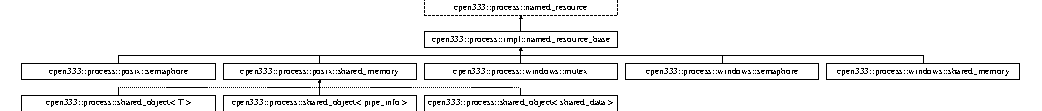
\includegraphics[height=11.872791cm]{classcpen333_1_1process_1_1impl_1_1named__resource__base}
\end{center}
\end{figure}
\subsection*{Public Member Functions}
\begin{DoxyCompactItemize}
\item 
\hyperlink{classcpen333_1_1process_1_1impl_1_1named__resource__base_a5f6f8b6daec88189a041de4c60ad4518}{named\+\_\+resource\+\_\+base} (const std\+::string \&\hyperlink{classcpen333_1_1process_1_1impl_1_1named__resource__base_a53986a0a1dd26a3602b842c45613b79d}{name})
\begin{DoxyCompactList}\small\item\em Constructor for base named resource. \end{DoxyCompactList}\item 
\mbox{\Hypertarget{classcpen333_1_1process_1_1impl_1_1named__resource__base_ae53d159d6c0d58a37ce8091aa132e11b}\label{classcpen333_1_1process_1_1impl_1_1named__resource__base_ae53d159d6c0d58a37ce8091aa132e11b}} 
virtual \hyperlink{classcpen333_1_1process_1_1impl_1_1named__resource__base_ae53d159d6c0d58a37ce8091aa132e11b}{$\sim$named\+\_\+resource\+\_\+base} ()
\begin{DoxyCompactList}\small\item\em Destructor, does nothing. \end{DoxyCompactList}\item 
std\+::string \hyperlink{classcpen333_1_1process_1_1impl_1_1named__resource__base_a53986a0a1dd26a3602b842c45613b79d}{name} ()
\begin{DoxyCompactList}\small\item\em Underlying name of resource. \end{DoxyCompactList}\item 
std\+::string \hyperlink{classcpen333_1_1process_1_1impl_1_1named__resource__base_abc636f266fcae871cec3861a90991898}{id} () const
\begin{DoxyCompactList}\small\item\em Internal-\/use system name. \end{DoxyCompactList}\item 
virtual bool \hyperlink{classcpen333_1_1process_1_1impl_1_1named__resource__base_ae4033f82dfd068b917a9bca57d3a0c45}{unlink} ()=0
\begin{DoxyCompactList}\small\item\em Detaches the name from the named resource. \end{DoxyCompactList}\end{DoxyCompactItemize}
\subsection*{Static Public Member Functions}
\begin{DoxyCompactItemize}
\item 
static bool \hyperlink{classcpen333_1_1process_1_1impl_1_1named__resource__base_a47a1396cf7c8210e76431a4ba4725146}{unlink} (const std\+::string \&\hyperlink{classcpen333_1_1process_1_1impl_1_1named__resource__base_a53986a0a1dd26a3602b842c45613b79d}{name})
\begin{DoxyCompactList}\small\item\em Unlinks the name without needing to create a resource. \end{DoxyCompactList}\end{DoxyCompactItemize}
\subsection*{Protected Member Functions}
\begin{DoxyCompactItemize}
\item 
void \hyperlink{classcpen333_1_1process_1_1impl_1_1named__resource__base_a46b07755d096da7295f6ba34355fad24}{set\+\_\+name} (const std\+::string \&\hyperlink{classcpen333_1_1process_1_1impl_1_1named__resource__base_a53986a0a1dd26a3602b842c45613b79d}{name})
\begin{DoxyCompactList}\small\item\em set\textquotesingle{}s the resource\textquotesingle{}s name \end{DoxyCompactList}\item 
const char $\ast$ \hyperlink{classcpen333_1_1process_1_1impl_1_1named__resource__base_a5291429a27070d875ca68bbf0a372842}{id\+\_\+ptr} () const
\begin{DoxyCompactList}\small\item\em Internal-\/use system name as char pointer. \end{DoxyCompactList}\end{DoxyCompactItemize}
\subsection*{Static Protected Member Functions}
\begin{DoxyCompactItemize}
\item 
static void \hyperlink{classcpen333_1_1process_1_1impl_1_1named__resource__base_a05acacbbb9c61cef11290c5e57432e18}{make\+\_\+resource\+\_\+id} (const std\+::string \&\hyperlink{classcpen333_1_1process_1_1impl_1_1named__resource__base_a53986a0a1dd26a3602b842c45613b79d}{name}, char $\ast$out)
\begin{DoxyCompactList}\small\item\em Creates a valid resource name. \end{DoxyCompactList}\end{DoxyCompactItemize}


\subsection{Detailed Description}
Base-\/class for named resources. 

Stores a unique identifier name 

\subsection{Constructor \& Destructor Documentation}
\mbox{\Hypertarget{classcpen333_1_1process_1_1impl_1_1named__resource__base_a5f6f8b6daec88189a041de4c60ad4518}\label{classcpen333_1_1process_1_1impl_1_1named__resource__base_a5f6f8b6daec88189a041de4c60ad4518}} 
\index{cpen333\+::process\+::impl\+::named\+\_\+resource\+\_\+base@{cpen333\+::process\+::impl\+::named\+\_\+resource\+\_\+base}!named\+\_\+resource\+\_\+base@{named\+\_\+resource\+\_\+base}}
\index{named\+\_\+resource\+\_\+base@{named\+\_\+resource\+\_\+base}!cpen333\+::process\+::impl\+::named\+\_\+resource\+\_\+base@{cpen333\+::process\+::impl\+::named\+\_\+resource\+\_\+base}}
\subsubsection{\texorpdfstring{named\+\_\+resource\+\_\+base()}{named\_resource\_base()}}
{\footnotesize\ttfamily cpen333\+::process\+::impl\+::named\+\_\+resource\+\_\+base\+::named\+\_\+resource\+\_\+base (\begin{DoxyParamCaption}\item[{const std\+::string \&}]{name }\end{DoxyParamCaption})\hspace{0.3cm}{\ttfamily [inline]}}



Constructor for base named resource. 


\begin{DoxyParams}{Parameters}
{\em name} & unique identifier \\
\hline
\end{DoxyParams}


\subsection{Member Function Documentation}
\mbox{\Hypertarget{classcpen333_1_1process_1_1impl_1_1named__resource__base_abc636f266fcae871cec3861a90991898}\label{classcpen333_1_1process_1_1impl_1_1named__resource__base_abc636f266fcae871cec3861a90991898}} 
\index{cpen333\+::process\+::impl\+::named\+\_\+resource\+\_\+base@{cpen333\+::process\+::impl\+::named\+\_\+resource\+\_\+base}!id@{id}}
\index{id@{id}!cpen333\+::process\+::impl\+::named\+\_\+resource\+\_\+base@{cpen333\+::process\+::impl\+::named\+\_\+resource\+\_\+base}}
\subsubsection{\texorpdfstring{id()}{id()}}
{\footnotesize\ttfamily std\+::string cpen333\+::process\+::impl\+::named\+\_\+resource\+\_\+base\+::id (\begin{DoxyParamCaption}{ }\end{DoxyParamCaption}) const\hspace{0.3cm}{\ttfamily [inline]}}



Internal-\/use system name. 

\begin{DoxyReturn}{Returns}
underlying unique identifier name 
\end{DoxyReturn}
\mbox{\Hypertarget{classcpen333_1_1process_1_1impl_1_1named__resource__base_a5291429a27070d875ca68bbf0a372842}\label{classcpen333_1_1process_1_1impl_1_1named__resource__base_a5291429a27070d875ca68bbf0a372842}} 
\index{cpen333\+::process\+::impl\+::named\+\_\+resource\+\_\+base@{cpen333\+::process\+::impl\+::named\+\_\+resource\+\_\+base}!id\+\_\+ptr@{id\+\_\+ptr}}
\index{id\+\_\+ptr@{id\+\_\+ptr}!cpen333\+::process\+::impl\+::named\+\_\+resource\+\_\+base@{cpen333\+::process\+::impl\+::named\+\_\+resource\+\_\+base}}
\subsubsection{\texorpdfstring{id\+\_\+ptr()}{id\_ptr()}}
{\footnotesize\ttfamily const char$\ast$ cpen333\+::process\+::impl\+::named\+\_\+resource\+\_\+base\+::id\+\_\+ptr (\begin{DoxyParamCaption}{ }\end{DoxyParamCaption}) const\hspace{0.3cm}{\ttfamily [inline]}, {\ttfamily [protected]}}



Internal-\/use system name as char pointer. 

\begin{DoxyReturn}{Returns}
pointer to underlying unique identifier name 
\end{DoxyReturn}
\mbox{\Hypertarget{classcpen333_1_1process_1_1impl_1_1named__resource__base_a05acacbbb9c61cef11290c5e57432e18}\label{classcpen333_1_1process_1_1impl_1_1named__resource__base_a05acacbbb9c61cef11290c5e57432e18}} 
\index{cpen333\+::process\+::impl\+::named\+\_\+resource\+\_\+base@{cpen333\+::process\+::impl\+::named\+\_\+resource\+\_\+base}!make\+\_\+resource\+\_\+id@{make\+\_\+resource\+\_\+id}}
\index{make\+\_\+resource\+\_\+id@{make\+\_\+resource\+\_\+id}!cpen333\+::process\+::impl\+::named\+\_\+resource\+\_\+base@{cpen333\+::process\+::impl\+::named\+\_\+resource\+\_\+base}}
\subsubsection{\texorpdfstring{make\+\_\+resource\+\_\+id()}{make\_resource\_id()}}
{\footnotesize\ttfamily static void cpen333\+::process\+::impl\+::named\+\_\+resource\+\_\+base\+::make\+\_\+resource\+\_\+id (\begin{DoxyParamCaption}\item[{const std\+::string \&}]{name,  }\item[{char $\ast$}]{out }\end{DoxyParamCaption})\hspace{0.3cm}{\ttfamily [inline]}, {\ttfamily [static]}, {\ttfamily [protected]}}



Creates a valid resource name. 

Creates a valid resource name for the platform, on Linux/\+O\+SX this is a leading \textquotesingle{}/\textquotesingle{} with sha1 base64-\/encoded hash of the string name. We will also replace any other \textquotesingle{}/\textquotesingle{} with \textquotesingle{}\+\_\+\textquotesingle{} 
\begin{DoxyParams}{Parameters}
{\em name} & original resource name \\
\hline
{\em out} & platform-\/safe resource name \\
\hline
\end{DoxyParams}
\mbox{\Hypertarget{classcpen333_1_1process_1_1impl_1_1named__resource__base_a53986a0a1dd26a3602b842c45613b79d}\label{classcpen333_1_1process_1_1impl_1_1named__resource__base_a53986a0a1dd26a3602b842c45613b79d}} 
\index{cpen333\+::process\+::impl\+::named\+\_\+resource\+\_\+base@{cpen333\+::process\+::impl\+::named\+\_\+resource\+\_\+base}!name@{name}}
\index{name@{name}!cpen333\+::process\+::impl\+::named\+\_\+resource\+\_\+base@{cpen333\+::process\+::impl\+::named\+\_\+resource\+\_\+base}}
\subsubsection{\texorpdfstring{name()}{name()}}
{\footnotesize\ttfamily std\+::string cpen333\+::process\+::impl\+::named\+\_\+resource\+\_\+base\+::name (\begin{DoxyParamCaption}{ }\end{DoxyParamCaption})\hspace{0.3cm}{\ttfamily [inline]}}



Underlying name of resource. 

\begin{DoxyReturn}{Returns}
resource name 
\end{DoxyReturn}
\mbox{\Hypertarget{classcpen333_1_1process_1_1impl_1_1named__resource__base_a46b07755d096da7295f6ba34355fad24}\label{classcpen333_1_1process_1_1impl_1_1named__resource__base_a46b07755d096da7295f6ba34355fad24}} 
\index{cpen333\+::process\+::impl\+::named\+\_\+resource\+\_\+base@{cpen333\+::process\+::impl\+::named\+\_\+resource\+\_\+base}!set\+\_\+name@{set\+\_\+name}}
\index{set\+\_\+name@{set\+\_\+name}!cpen333\+::process\+::impl\+::named\+\_\+resource\+\_\+base@{cpen333\+::process\+::impl\+::named\+\_\+resource\+\_\+base}}
\subsubsection{\texorpdfstring{set\+\_\+name()}{set\_name()}}
{\footnotesize\ttfamily void cpen333\+::process\+::impl\+::named\+\_\+resource\+\_\+base\+::set\+\_\+name (\begin{DoxyParamCaption}\item[{const std\+::string \&}]{name }\end{DoxyParamCaption})\hspace{0.3cm}{\ttfamily [inline]}, {\ttfamily [protected]}}



set\textquotesingle{}s the resource\textquotesingle{}s name 


\begin{DoxyParams}{Parameters}
{\em name} & \\
\hline
\end{DoxyParams}
\mbox{\Hypertarget{classcpen333_1_1process_1_1impl_1_1named__resource__base_ae4033f82dfd068b917a9bca57d3a0c45}\label{classcpen333_1_1process_1_1impl_1_1named__resource__base_ae4033f82dfd068b917a9bca57d3a0c45}} 
\index{cpen333\+::process\+::impl\+::named\+\_\+resource\+\_\+base@{cpen333\+::process\+::impl\+::named\+\_\+resource\+\_\+base}!unlink@{unlink}}
\index{unlink@{unlink}!cpen333\+::process\+::impl\+::named\+\_\+resource\+\_\+base@{cpen333\+::process\+::impl\+::named\+\_\+resource\+\_\+base}}
\subsubsection{\texorpdfstring{unlink()}{unlink()}\hspace{0.1cm}{\footnotesize\ttfamily [1/2]}}
{\footnotesize\ttfamily virtual bool cpen333\+::process\+::impl\+::named\+\_\+resource\+\_\+base\+::unlink (\begin{DoxyParamCaption}{ }\end{DoxyParamCaption})\hspace{0.3cm}{\ttfamily [pure virtual]}}



Detaches the name from the named resource. 

On P\+O\+S\+IX systems, named resources will persist beyond the lifetime of any process that uses them as long as the name has not been unlinked (or until the system is rebooted). Calling {\ttfamily unlink} will detach the name, allowing the resource to be freed once all current users have exited.

\begin{DoxyReturn}{Returns}
{\ttfamily true} if unlink is successful, {\ttfamily false} if unlinking is not supported or if an error has occurred. 
\end{DoxyReturn}


Implements \hyperlink{classcpen333_1_1process_1_1named__resource_a5d33168fee48c9b0c58ab8fd96e230ce}{cpen333\+::process\+::named\+\_\+resource}.



Implemented in \hyperlink{classcpen333_1_1process_1_1posix_1_1pipe__server_a5c4da1864cb0db53e76d960230f3a83a}{cpen333\+::process\+::posix\+::pipe\+\_\+server}, \hyperlink{classcpen333_1_1process_1_1windows_1_1pipe__server_aa3f9fb4fd88042b09e130cd616815fe1}{cpen333\+::process\+::windows\+::pipe\+\_\+server}, \hyperlink{classcpen333_1_1process_1_1posix_1_1pipe_ac1dd8e1a7fd46480b709e96190afe697}{cpen333\+::process\+::posix\+::pipe}, \hyperlink{classcpen333_1_1process_1_1windows_1_1pipe_abe0bc707040aa7e82ed41c26cc4c93c1}{cpen333\+::process\+::windows\+::pipe}, \hyperlink{classcpen333_1_1process_1_1posix_1_1semaphore_aa6064e2c4b4b7282cc5e6eda877ee1bb}{cpen333\+::process\+::posix\+::semaphore}, \hyperlink{classcpen333_1_1process_1_1windows_1_1semaphore_abc5159f32e61024c6c6a978ac64fe39d}{cpen333\+::process\+::windows\+::semaphore}, \hyperlink{classcpen333_1_1process_1_1posix_1_1shared__memory_a3b6d67a41cfaca3712d87958682d8bbe}{cpen333\+::process\+::posix\+::shared\+\_\+memory}, \hyperlink{classcpen333_1_1process_1_1windows_1_1shared__memory_aa6efdc9a3e1310ea69ecc48aeb41286c}{cpen333\+::process\+::windows\+::shared\+\_\+memory}, \hyperlink{classcpen333_1_1process_1_1windows_1_1mutex_aa45381a0a226fbefc86eef8971a5431b}{cpen333\+::process\+::windows\+::mutex}, \hyperlink{classcpen333_1_1process_1_1posix_1_1mutex_ac1bcf9576d7470e5d64e17876c9cdb36}{cpen333\+::process\+::posix\+::mutex}, \hyperlink{classcpen333_1_1process_1_1shared__object_aa5b43829da5bd2376927e6285745211c}{cpen333\+::process\+::shared\+\_\+object$<$ T $>$}, \hyperlink{classcpen333_1_1process_1_1shared__object_aa5b43829da5bd2376927e6285745211c}{cpen333\+::process\+::shared\+\_\+object$<$ pipe\+\_\+info $>$}, and \hyperlink{classcpen333_1_1process_1_1shared__object_aa5b43829da5bd2376927e6285745211c}{cpen333\+::process\+::shared\+\_\+object$<$ shared\+\_\+data $>$}.

\mbox{\Hypertarget{classcpen333_1_1process_1_1impl_1_1named__resource__base_a47a1396cf7c8210e76431a4ba4725146}\label{classcpen333_1_1process_1_1impl_1_1named__resource__base_a47a1396cf7c8210e76431a4ba4725146}} 
\index{cpen333\+::process\+::impl\+::named\+\_\+resource\+\_\+base@{cpen333\+::process\+::impl\+::named\+\_\+resource\+\_\+base}!unlink@{unlink}}
\index{unlink@{unlink}!cpen333\+::process\+::impl\+::named\+\_\+resource\+\_\+base@{cpen333\+::process\+::impl\+::named\+\_\+resource\+\_\+base}}
\subsubsection{\texorpdfstring{unlink()}{unlink()}\hspace{0.1cm}{\footnotesize\ttfamily [2/2]}}
{\footnotesize\ttfamily static bool cpen333\+::process\+::impl\+::named\+\_\+resource\+\_\+base\+::unlink (\begin{DoxyParamCaption}\item[{const std\+::string \&}]{name }\end{DoxyParamCaption})\hspace{0.3cm}{\ttfamily [inline]}, {\ttfamily [static]}}



Unlinks the name without needing to create a resource. 

Implementers should also provide a static method for unlinking. The purpose is mainly for clean-\/up of existing resources.


\begin{DoxyParams}{Parameters}
{\em name} & desired resource name \\
\hline
\end{DoxyParams}
\begin{DoxyReturn}{Returns}
{\ttfamily true} if unlink successful, {\ttfamily false} if not successful or not supported 
\end{DoxyReturn}


The documentation for this class was generated from the following file\+:\begin{DoxyCompactItemize}
\item 
D\+:/school/teaching/\+C\+P\+E\+N333/workspace/library/include/cpen333/process/impl/\hyperlink{named__resource__base_8h}{named\+\_\+resource\+\_\+base.\+h}\end{DoxyCompactItemize}

\hypertarget{classcpen333_1_1process_1_1pipe}{}\section{cpen333\+:\+:process\+:\+:pipe Class Reference}
\label{classcpen333_1_1process_1_1pipe}\index{cpen333\+::process\+::pipe@{cpen333\+::process\+::pipe}}


A client pipe implementation for inter-\/process communication.  




{\ttfamily \#include $<$pipe.\+h$>$}



\subsection{Detailed Description}
A client pipe implementation for inter-\/process communication. 

Used to communicate between processes on the same machine over a bi-\/directional channel. This is an alias to either \hyperlink{classcpen333_1_1process_1_1posix_1_1pipe}{cpen333\+::process\+::posix\+::pipe} or \hyperlink{classcpen333_1_1process_1_1windows_1_1pipe}{cpen333\+::process\+::windows\+::pipe} depending on your platform. 

The documentation for this class was generated from the following file\+:\begin{DoxyCompactItemize}
\item 
D\+:/school/teaching/\+C\+P\+E\+N333/workspace/library/include/cpen333/process/\hyperlink{pipe_8h}{pipe.\+h}\end{DoxyCompactItemize}

\input{classcpen333_1_1process_1_1rendezvous}
\input{classcpen333_1_1thread_1_1rendezvous}
\input{classcpen333_1_1process_1_1semaphore}
\hypertarget{classcpen333_1_1process_1_1windows_1_1semaphore}{}\section{cpen333\+:\+:process\+:\+:windows\+:\+:semaphore Class Reference}
\label{classcpen333_1_1process_1_1windows_1_1semaphore}\index{cpen333\+::process\+::windows\+::semaphore@{cpen333\+::process\+::windows\+::semaphore}}


Inter-\/process named semaphore primitive.  




{\ttfamily \#include $<$semaphore.\+h$>$}

Inheritance diagram for cpen333\+:\+:process\+:\+:windows\+:\+:semaphore\+:\begin{figure}[H]
\begin{center}
\leavevmode
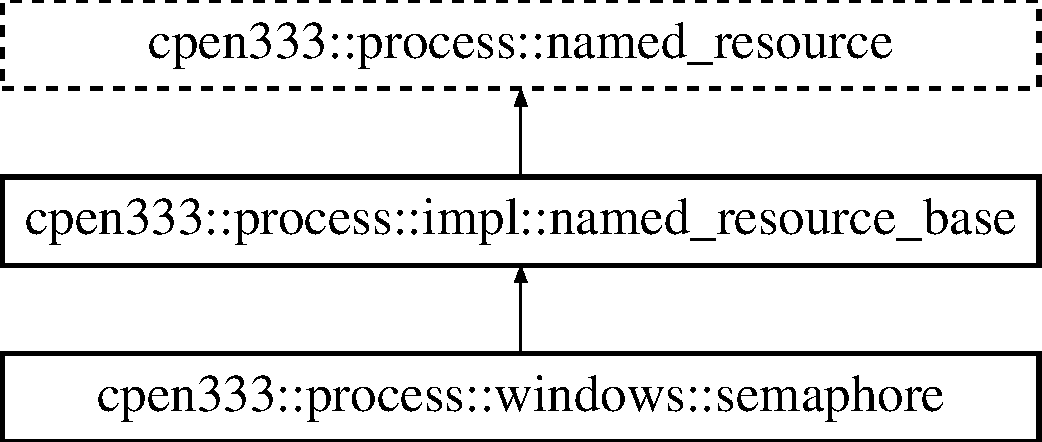
\includegraphics[height=3.000000cm]{classcpen333_1_1process_1_1windows_1_1semaphore}
\end{center}
\end{figure}
\subsection*{Public Types}
\begin{DoxyCompactItemize}
\item 
typedef H\+A\+N\+D\+LE \hyperlink{classcpen333_1_1process_1_1windows_1_1semaphore_a07f523e9a1edf0ae8afa2f21487a1953}{native\+\_\+handle\+\_\+type}
\begin{DoxyCompactList}\small\item\em Alias to native handle type for semaphore. \end{DoxyCompactList}\end{DoxyCompactItemize}
\subsection*{Public Member Functions}
\begin{DoxyCompactItemize}
\item 
\hyperlink{classcpen333_1_1process_1_1windows_1_1semaphore_a1bd71d0b00c26143be3187c18ec6865a}{semaphore} (const std\+::string \&\hyperlink{classcpen333_1_1process_1_1impl_1_1named__resource__base_a53986a0a1dd26a3602b842c45613b79d}{name}, size\+\_\+t \hyperlink{classcpen333_1_1process_1_1windows_1_1semaphore_a15245feed98e3cf8a428c0a218f33012}{value}=1)
\begin{DoxyCompactList}\small\item\em Constructs or connects to a named semaphore. \end{DoxyCompactList}\item 
\mbox{\Hypertarget{classcpen333_1_1process_1_1windows_1_1semaphore_a10260478f3b3732d4a52499385ad6575}\label{classcpen333_1_1process_1_1windows_1_1semaphore_a10260478f3b3732d4a52499385ad6575}} 
\hyperlink{classcpen333_1_1process_1_1windows_1_1semaphore_a10260478f3b3732d4a52499385ad6575}{$\sim$semaphore} ()
\begin{DoxyCompactList}\small\item\em Destructor. \end{DoxyCompactList}\item 
size\+\_\+t \hyperlink{classcpen333_1_1process_1_1windows_1_1semaphore_a15245feed98e3cf8a428c0a218f33012}{value} ()
\begin{DoxyCompactList}\small\item\em Determines the current stored value of the semaphore. \end{DoxyCompactList}\item 
void \hyperlink{classcpen333_1_1process_1_1windows_1_1semaphore_a523d89b784ed47ade79d4ecf836f042d}{wait} ()
\begin{DoxyCompactList}\small\item\em Waits for and decrements the semaphore value. \end{DoxyCompactList}\item 
bool \hyperlink{classcpen333_1_1process_1_1windows_1_1semaphore_a06cffd6c2ed120af0477252fb48b0346}{try\+\_\+wait} ()
\begin{DoxyCompactList}\small\item\em Tries to wait for the semaphore, returning immediately. \end{DoxyCompactList}\item 
{\footnotesize template$<$class Rep , class Period $>$ }\\bool \hyperlink{classcpen333_1_1process_1_1windows_1_1semaphore_a055c5a6ec94b231b04856ba78862b0ee}{wait\+\_\+for} (const std\+::chrono\+::duration$<$ Rep, Period $>$ \&timeout\+\_\+duration)
\begin{DoxyCompactList}\small\item\em Tries to wait for the semaphore for up to a maximum timeout duration. \end{DoxyCompactList}\item 
{\footnotesize template$<$class Clock , class Duration $>$ }\\bool \hyperlink{classcpen333_1_1process_1_1windows_1_1semaphore_a2264a9d3557c6507b6c2e37599bd3f83}{wait\+\_\+until} (const std\+::chrono\+::time\+\_\+point$<$ Clock, Duration $>$ \&timeout\+\_\+time)
\begin{DoxyCompactList}\small\item\em Tries to wait for the semaphore for up to a maximum absolute time. \end{DoxyCompactList}\item 
void \hyperlink{classcpen333_1_1process_1_1windows_1_1semaphore_a7f1443d55e1112e7b2a15334bafc958b}{notify} ()
\begin{DoxyCompactList}\small\item\em Increments the semaphore value. \end{DoxyCompactList}\item 
\hyperlink{classcpen333_1_1process_1_1windows_1_1semaphore_a07f523e9a1edf0ae8afa2f21487a1953}{native\+\_\+handle\+\_\+type} \hyperlink{classcpen333_1_1process_1_1windows_1_1semaphore_ae73fa406be3b0df603b260e892c94081}{native\+\_\+handle} ()
\begin{DoxyCompactList}\small\item\em Returns a native handle to the semaphore. \end{DoxyCompactList}\item 
bool \hyperlink{classcpen333_1_1process_1_1windows_1_1semaphore_abc5159f32e61024c6c6a978ac64fe39d}{unlink} ()
\begin{DoxyCompactList}\small\item\em Detaches the name from the named resource. \end{DoxyCompactList}\end{DoxyCompactItemize}
\subsection*{Static Public Member Functions}
\begin{DoxyCompactItemize}
\item 
static bool \hyperlink{classcpen333_1_1process_1_1windows_1_1semaphore_ae3837124e878a66370b7e1931c6b1bf8}{unlink} (const std\+::string \&\hyperlink{classcpen333_1_1process_1_1impl_1_1named__resource__base_a53986a0a1dd26a3602b842c45613b79d}{name})
\begin{DoxyCompactList}\small\item\em Unlinks the name without needing to create a resource. \end{DoxyCompactList}\end{DoxyCompactItemize}
\subsection*{Additional Inherited Members}


\subsection{Detailed Description}
Inter-\/process named semaphore primitive. 

Used to limit access to a number of resources. Contains an integer whose value is never allowed to fall below zero. There are two main supported actions\+: \hyperlink{classcpen333_1_1process_1_1windows_1_1semaphore_a523d89b784ed47ade79d4ecf836f042d}{wait()}, which decrements the internal value, and \hyperlink{classcpen333_1_1process_1_1windows_1_1semaphore_a7f1443d55e1112e7b2a15334bafc958b}{notify()} which increments the value. If the value of the semaphore is zero, then \hyperlink{classcpen333_1_1process_1_1windows_1_1semaphore_a523d89b784ed47ade79d4ecf836f042d}{wait()} will cause the thread to block until the value becomes greater than zero.

This implementation has no explicit maximum value

This semaphore has U\+S\+A\+GE P\+E\+R\+S\+I\+S\+T\+E\+N\+CE, meaning the mutex will continue to exist as long as at least one process/thread is holding a reference to it. 

\subsection{Member Typedef Documentation}
\mbox{\Hypertarget{classcpen333_1_1process_1_1windows_1_1semaphore_a07f523e9a1edf0ae8afa2f21487a1953}\label{classcpen333_1_1process_1_1windows_1_1semaphore_a07f523e9a1edf0ae8afa2f21487a1953}} 
\index{cpen333\+::process\+::windows\+::semaphore@{cpen333\+::process\+::windows\+::semaphore}!native\+\_\+handle\+\_\+type@{native\+\_\+handle\+\_\+type}}
\index{native\+\_\+handle\+\_\+type@{native\+\_\+handle\+\_\+type}!cpen333\+::process\+::windows\+::semaphore@{cpen333\+::process\+::windows\+::semaphore}}
\subsubsection{\texorpdfstring{native\+\_\+handle\+\_\+type}{native\_handle\_type}}
{\footnotesize\ttfamily typedef H\+A\+N\+D\+LE \hyperlink{classcpen333_1_1process_1_1posix_1_1semaphore_ad63150e5c8c196a84a7b214462756f1a}{cpen333\+::process\+::windows\+::semaphore\+::native\+\_\+handle\+\_\+type}}



Alias to native handle type for semaphore. 

In this case, a Windows H\+A\+N\+D\+LE to a Semaphore 

\subsection{Constructor \& Destructor Documentation}
\mbox{\Hypertarget{classcpen333_1_1process_1_1windows_1_1semaphore_a1bd71d0b00c26143be3187c18ec6865a}\label{classcpen333_1_1process_1_1windows_1_1semaphore_a1bd71d0b00c26143be3187c18ec6865a}} 
\index{cpen333\+::process\+::windows\+::semaphore@{cpen333\+::process\+::windows\+::semaphore}!semaphore@{semaphore}}
\index{semaphore@{semaphore}!cpen333\+::process\+::windows\+::semaphore@{cpen333\+::process\+::windows\+::semaphore}}
\subsubsection{\texorpdfstring{semaphore()}{semaphore()}}
{\footnotesize\ttfamily cpen333\+::process\+::windows\+::semaphore\+::semaphore (\begin{DoxyParamCaption}\item[{const std\+::string \&}]{name,  }\item[{size\+\_\+t}]{value = {\ttfamily 1} }\end{DoxyParamCaption})\hspace{0.3cm}{\ttfamily [inline]}}



Constructs or connects to a named semaphore. 


\begin{DoxyParams}{Parameters}
{\em name} & identifier for creating or connecting to an existing inter-\/process semaphore \\
\hline
{\em value} & initial value (defaults to 1) \\
\hline
\end{DoxyParams}


\subsection{Member Function Documentation}
\mbox{\Hypertarget{classcpen333_1_1process_1_1windows_1_1semaphore_ae73fa406be3b0df603b260e892c94081}\label{classcpen333_1_1process_1_1windows_1_1semaphore_ae73fa406be3b0df603b260e892c94081}} 
\index{cpen333\+::process\+::windows\+::semaphore@{cpen333\+::process\+::windows\+::semaphore}!native\+\_\+handle@{native\+\_\+handle}}
\index{native\+\_\+handle@{native\+\_\+handle}!cpen333\+::process\+::windows\+::semaphore@{cpen333\+::process\+::windows\+::semaphore}}
\subsubsection{\texorpdfstring{native\+\_\+handle()}{native\_handle()}}
{\footnotesize\ttfamily \hyperlink{classcpen333_1_1process_1_1windows_1_1semaphore_a07f523e9a1edf0ae8afa2f21487a1953}{native\+\_\+handle\+\_\+type} cpen333\+::process\+::windows\+::semaphore\+::native\+\_\+handle (\begin{DoxyParamCaption}{ }\end{DoxyParamCaption})\hspace{0.3cm}{\ttfamily [inline]}}



Returns a native handle to the semaphore. 

The native handle has a type aliased to \hyperlink{classcpen333_1_1process_1_1windows_1_1semaphore_a07f523e9a1edf0ae8afa2f21487a1953}{semaphore\+::native\+\_\+handle\+\_\+type}

On Windows systems, is of type H\+A\+N\+D\+LE to a Semaphore.

\begin{DoxyReturn}{Returns}
native semaphore handle 
\end{DoxyReturn}
\mbox{\Hypertarget{classcpen333_1_1process_1_1windows_1_1semaphore_a7f1443d55e1112e7b2a15334bafc958b}\label{classcpen333_1_1process_1_1windows_1_1semaphore_a7f1443d55e1112e7b2a15334bafc958b}} 
\index{cpen333\+::process\+::windows\+::semaphore@{cpen333\+::process\+::windows\+::semaphore}!notify@{notify}}
\index{notify@{notify}!cpen333\+::process\+::windows\+::semaphore@{cpen333\+::process\+::windows\+::semaphore}}
\subsubsection{\texorpdfstring{notify()}{notify()}}
{\footnotesize\ttfamily void cpen333\+::process\+::windows\+::semaphore\+::notify (\begin{DoxyParamCaption}{ }\end{DoxyParamCaption})\hspace{0.3cm}{\ttfamily [inline]}}



Increments the semaphore value. 

If the semaphore\textquotesingle{}s value consequently becomes greater than zero, then one process or thread that is currently blocked in a \hyperlink{classcpen333_1_1process_1_1windows_1_1semaphore_a523d89b784ed47ade79d4ecf836f042d}{wait()} operation will be woken up and will proceed. \mbox{\Hypertarget{classcpen333_1_1process_1_1windows_1_1semaphore_a06cffd6c2ed120af0477252fb48b0346}\label{classcpen333_1_1process_1_1windows_1_1semaphore_a06cffd6c2ed120af0477252fb48b0346}} 
\index{cpen333\+::process\+::windows\+::semaphore@{cpen333\+::process\+::windows\+::semaphore}!try\+\_\+wait@{try\+\_\+wait}}
\index{try\+\_\+wait@{try\+\_\+wait}!cpen333\+::process\+::windows\+::semaphore@{cpen333\+::process\+::windows\+::semaphore}}
\subsubsection{\texorpdfstring{try\+\_\+wait()}{try\_wait()}}
{\footnotesize\ttfamily bool cpen333\+::process\+::windows\+::semaphore\+::try\+\_\+wait (\begin{DoxyParamCaption}{ }\end{DoxyParamCaption})\hspace{0.3cm}{\ttfamily [inline]}}



Tries to wait for the semaphore, returning immediately. 

If the value is greater than zero, will decrement the semaphore and return true. Otherwise, will return false.

\begin{DoxyReturn}{Returns}
true if decrement successful, false otherwise 
\end{DoxyReturn}
\mbox{\Hypertarget{classcpen333_1_1process_1_1windows_1_1semaphore_abc5159f32e61024c6c6a978ac64fe39d}\label{classcpen333_1_1process_1_1windows_1_1semaphore_abc5159f32e61024c6c6a978ac64fe39d}} 
\index{cpen333\+::process\+::windows\+::semaphore@{cpen333\+::process\+::windows\+::semaphore}!unlink@{unlink}}
\index{unlink@{unlink}!cpen333\+::process\+::windows\+::semaphore@{cpen333\+::process\+::windows\+::semaphore}}
\subsubsection{\texorpdfstring{unlink()}{unlink()}\hspace{0.1cm}{\footnotesize\ttfamily [1/2]}}
{\footnotesize\ttfamily bool cpen333\+::process\+::windows\+::semaphore\+::unlink (\begin{DoxyParamCaption}{ }\end{DoxyParamCaption})\hspace{0.3cm}{\ttfamily [inline]}, {\ttfamily [virtual]}}



Detaches the name from the named resource. 

On P\+O\+S\+IX systems, named resources will persist beyond the lifetime of any process that uses them as long as the name has not been unlinked (or until the system is rebooted). Calling {\ttfamily unlink} will detach the name, allowing the resource to be freed once all current users have exited.

\begin{DoxyReturn}{Returns}
{\ttfamily true} if unlink is successful, {\ttfamily false} if unlinking is not supported or if an error has occurred. 
\end{DoxyReturn}


Implements \hyperlink{classcpen333_1_1process_1_1impl_1_1named__resource__base_ae4033f82dfd068b917a9bca57d3a0c45}{cpen333\+::process\+::impl\+::named\+\_\+resource\+\_\+base}.

\mbox{\Hypertarget{classcpen333_1_1process_1_1windows_1_1semaphore_ae3837124e878a66370b7e1931c6b1bf8}\label{classcpen333_1_1process_1_1windows_1_1semaphore_ae3837124e878a66370b7e1931c6b1bf8}} 
\index{cpen333\+::process\+::windows\+::semaphore@{cpen333\+::process\+::windows\+::semaphore}!unlink@{unlink}}
\index{unlink@{unlink}!cpen333\+::process\+::windows\+::semaphore@{cpen333\+::process\+::windows\+::semaphore}}
\subsubsection{\texorpdfstring{unlink()}{unlink()}\hspace{0.1cm}{\footnotesize\ttfamily [2/2]}}
{\footnotesize\ttfamily static bool cpen333\+::process\+::windows\+::semaphore\+::unlink (\begin{DoxyParamCaption}\item[{const std\+::string \&}]{name }\end{DoxyParamCaption})\hspace{0.3cm}{\ttfamily [inline]}, {\ttfamily [static]}}



Unlinks the name without needing to create a resource. 

Implementers should also provide a static method for unlinking. The purpose is mainly for clean-\/up of existing resources.


\begin{DoxyParams}{Parameters}
{\em name} & desired resource name \\
\hline
\end{DoxyParams}
\begin{DoxyReturn}{Returns}
{\ttfamily true} if unlink successful, {\ttfamily false} if not successful or not supported 
\end{DoxyReturn}
\mbox{\Hypertarget{classcpen333_1_1process_1_1windows_1_1semaphore_a15245feed98e3cf8a428c0a218f33012}\label{classcpen333_1_1process_1_1windows_1_1semaphore_a15245feed98e3cf8a428c0a218f33012}} 
\index{cpen333\+::process\+::windows\+::semaphore@{cpen333\+::process\+::windows\+::semaphore}!value@{value}}
\index{value@{value}!cpen333\+::process\+::windows\+::semaphore@{cpen333\+::process\+::windows\+::semaphore}}
\subsubsection{\texorpdfstring{value()}{value()}}
{\footnotesize\ttfamily size\+\_\+t cpen333\+::process\+::windows\+::semaphore\+::value (\begin{DoxyParamCaption}{ }\end{DoxyParamCaption})\hspace{0.3cm}{\ttfamily [inline]}}



Determines the current stored value of the semaphore. 

This should never be used, except for possibly debugging, as the value may change without notice from other threads. This method will cause an error on O\+SX.

\begin{DoxyReturn}{Returns}

\end{DoxyReturn}
\mbox{\Hypertarget{classcpen333_1_1process_1_1windows_1_1semaphore_a523d89b784ed47ade79d4ecf836f042d}\label{classcpen333_1_1process_1_1windows_1_1semaphore_a523d89b784ed47ade79d4ecf836f042d}} 
\index{cpen333\+::process\+::windows\+::semaphore@{cpen333\+::process\+::windows\+::semaphore}!wait@{wait}}
\index{wait@{wait}!cpen333\+::process\+::windows\+::semaphore@{cpen333\+::process\+::windows\+::semaphore}}
\subsubsection{\texorpdfstring{wait()}{wait()}}
{\footnotesize\ttfamily void cpen333\+::process\+::windows\+::semaphore\+::wait (\begin{DoxyParamCaption}{ }\end{DoxyParamCaption})\hspace{0.3cm}{\ttfamily [inline]}}



Waits for and decrements the semaphore value. 

If the value is greater than zero, will decrement it and return immediately. Otherwise, the thread will block until it becomes possible to perform the decrement. \mbox{\Hypertarget{classcpen333_1_1process_1_1windows_1_1semaphore_a055c5a6ec94b231b04856ba78862b0ee}\label{classcpen333_1_1process_1_1windows_1_1semaphore_a055c5a6ec94b231b04856ba78862b0ee}} 
\index{cpen333\+::process\+::windows\+::semaphore@{cpen333\+::process\+::windows\+::semaphore}!wait\+\_\+for@{wait\+\_\+for}}
\index{wait\+\_\+for@{wait\+\_\+for}!cpen333\+::process\+::windows\+::semaphore@{cpen333\+::process\+::windows\+::semaphore}}
\subsubsection{\texorpdfstring{wait\+\_\+for()}{wait\_for()}}
{\footnotesize\ttfamily template$<$class Rep , class Period $>$ \\
bool cpen333\+::process\+::windows\+::semaphore\+::wait\+\_\+for (\begin{DoxyParamCaption}\item[{const std\+::chrono\+::duration$<$ Rep, Period $>$ \&}]{timeout\+\_\+duration }\end{DoxyParamCaption})\hspace{0.3cm}{\ttfamily [inline]}}



Tries to wait for the semaphore for up to a maximum timeout duration. 

If the semaphore\textquotesingle{}s value is greater than zero, will decrement it and return true immediately. Otherwise, will wait (blocking) up to a maximum relative timeout period.


\begin{DoxyTemplParams}{Template Parameters}
{\em Rep} & time representation \\
\hline
{\em Period} & timeout period type \\
\hline
\end{DoxyTemplParams}

\begin{DoxyParams}{Parameters}
{\em timeout\+\_\+duration} & maximum relative duration for waiting \\
\hline
\end{DoxyParams}
\begin{DoxyReturn}{Returns}
true if semaphore successfully decremented, false if timed-\/out 
\end{DoxyReturn}
\mbox{\Hypertarget{classcpen333_1_1process_1_1windows_1_1semaphore_a2264a9d3557c6507b6c2e37599bd3f83}\label{classcpen333_1_1process_1_1windows_1_1semaphore_a2264a9d3557c6507b6c2e37599bd3f83}} 
\index{cpen333\+::process\+::windows\+::semaphore@{cpen333\+::process\+::windows\+::semaphore}!wait\+\_\+until@{wait\+\_\+until}}
\index{wait\+\_\+until@{wait\+\_\+until}!cpen333\+::process\+::windows\+::semaphore@{cpen333\+::process\+::windows\+::semaphore}}
\subsubsection{\texorpdfstring{wait\+\_\+until()}{wait\_until()}}
{\footnotesize\ttfamily template$<$class Clock , class Duration $>$ \\
bool cpen333\+::process\+::windows\+::semaphore\+::wait\+\_\+until (\begin{DoxyParamCaption}\item[{const std\+::chrono\+::time\+\_\+point$<$ Clock, Duration $>$ \&}]{timeout\+\_\+time }\end{DoxyParamCaption})\hspace{0.3cm}{\ttfamily [inline]}}



Tries to wait for the semaphore for up to a maximum absolute time. 

If the semaphore\textquotesingle{}s value is greater than zero, will decrement it and return true immediately. Otherwise, will wait (blocking) up to a maximum relative timeout period.


\begin{DoxyTemplParams}{Template Parameters}
{\em Clock} & timeout clock type \\
\hline
{\em Duration} & timeout duration type \\
\hline
\end{DoxyTemplParams}

\begin{DoxyParams}{Parameters}
{\em timeout\+\_\+time} & maximum absolute time for waiting \\
\hline
\end{DoxyParams}
\begin{DoxyReturn}{Returns}
true if semaphore successfully decremented, false if timed-\/out 
\end{DoxyReturn}


The documentation for this class was generated from the following file\+:\begin{DoxyCompactItemize}
\item 
D\+:/school/teaching/\+C\+P\+E\+N333/workspace/library/include/cpen333/process/impl/windows/\hyperlink{process_2impl_2windows_2semaphore_8h}{semaphore.\+h}\end{DoxyCompactItemize}

\hypertarget{classcpen333_1_1process_1_1posix_1_1semaphore}{}\section{cpen333\+:\+:process\+:\+:posix\+:\+:semaphore Class Reference}
\label{classcpen333_1_1process_1_1posix_1_1semaphore}\index{cpen333\+::process\+::posix\+::semaphore@{cpen333\+::process\+::posix\+::semaphore}}


Inter-\/process named semaphore primitive.  




{\ttfamily \#include $<$semaphore.\+h$>$}

Inheritance diagram for cpen333\+:\+:process\+:\+:posix\+:\+:semaphore\+:\begin{figure}[H]
\begin{center}
\leavevmode
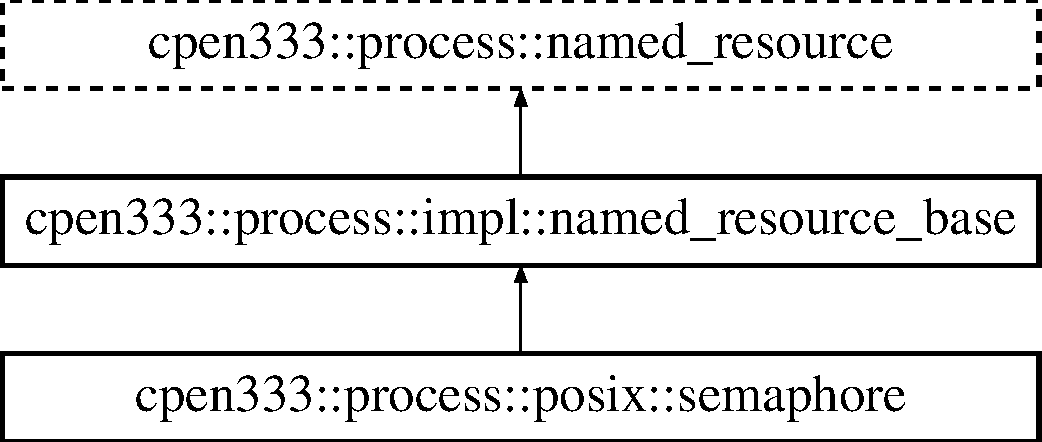
\includegraphics[height=3.000000cm]{classcpen333_1_1process_1_1posix_1_1semaphore}
\end{center}
\end{figure}
\subsection*{Public Types}
\begin{DoxyCompactItemize}
\item 
using \hyperlink{classcpen333_1_1process_1_1posix_1_1semaphore_ad63150e5c8c196a84a7b214462756f1a}{native\+\_\+handle\+\_\+type} = sem\+\_\+t $\ast$
\begin{DoxyCompactList}\small\item\em Alias to native handle type for semaphore. \end{DoxyCompactList}\end{DoxyCompactItemize}
\subsection*{Public Member Functions}
\begin{DoxyCompactItemize}
\item 
\hyperlink{classcpen333_1_1process_1_1posix_1_1semaphore_aee6d65abd5bbfcfd1629140cb20c8ad1}{semaphore} (const std\+::string \&\hyperlink{classcpen333_1_1process_1_1impl_1_1named__resource__base_a53986a0a1dd26a3602b842c45613b79d}{name}, size\+\_\+t \hyperlink{classcpen333_1_1process_1_1posix_1_1semaphore_a336211ff42ee9da6315c76104840fa98}{value}=1)
\begin{DoxyCompactList}\small\item\em Constructs or connects to a named semaphore. \end{DoxyCompactList}\item 
\mbox{\Hypertarget{classcpen333_1_1process_1_1posix_1_1semaphore_a9c32f8d2192cca78b7415f9e3af056a6}\label{classcpen333_1_1process_1_1posix_1_1semaphore_a9c32f8d2192cca78b7415f9e3af056a6}} 
\hyperlink{classcpen333_1_1process_1_1posix_1_1semaphore_a9c32f8d2192cca78b7415f9e3af056a6}{$\sim$semaphore} ()
\begin{DoxyCompactList}\small\item\em Destructor. \end{DoxyCompactList}\item 
size\+\_\+t \hyperlink{classcpen333_1_1process_1_1posix_1_1semaphore_a336211ff42ee9da6315c76104840fa98}{value} ()
\begin{DoxyCompactList}\small\item\em Determines the current stored value of the semaphore. \end{DoxyCompactList}\item 
void \hyperlink{classcpen333_1_1process_1_1posix_1_1semaphore_a1cf2d5f5922ab6358061dd3ac7121cf9}{wait} ()
\begin{DoxyCompactList}\small\item\em Waits for and decrements the semaphore value. \end{DoxyCompactList}\item 
bool \hyperlink{classcpen333_1_1process_1_1posix_1_1semaphore_ac0e2bd6495113c0699c5e2511f345edb}{try\+\_\+wait} ()
\begin{DoxyCompactList}\small\item\em Tries to wait for the semaphore, returning immediately. \end{DoxyCompactList}\item 
void \hyperlink{classcpen333_1_1process_1_1posix_1_1semaphore_a1b9043106c5da18ad152bc83e3de1750}{notify} ()
\begin{DoxyCompactList}\small\item\em Increments the semaphore value. \end{DoxyCompactList}\item 
{\footnotesize template$<$class Rep , class Period $>$ }\\bool \hyperlink{classcpen333_1_1process_1_1posix_1_1semaphore_a8015c878067c3d93748d03c58bb1b233}{wait\+\_\+for} (const std\+::chrono\+::duration$<$ Rep, Period $>$ \&timeout\+\_\+duration)
\begin{DoxyCompactList}\small\item\em Tries to wait for the semaphore for up to a maximum timeout duration. \end{DoxyCompactList}\item 
{\footnotesize template$<$class Clock , class Duration $>$ }\\bool \hyperlink{classcpen333_1_1process_1_1posix_1_1semaphore_a83443f24c1b7b11e5384975e9abc77dc}{wait\+\_\+until} (const std\+::chrono\+::time\+\_\+point$<$ Clock, Duration $>$ \&timeout\+\_\+time)
\begin{DoxyCompactList}\small\item\em Tries to wait for the semaphore for up to a maximum absolute time. \end{DoxyCompactList}\item 
\hyperlink{classcpen333_1_1process_1_1posix_1_1semaphore_ad63150e5c8c196a84a7b214462756f1a}{native\+\_\+handle\+\_\+type} \hyperlink{classcpen333_1_1process_1_1posix_1_1semaphore_a1e4a2d5a032a71fc06a5065f0e83a94c}{native\+\_\+handle} () const
\begin{DoxyCompactList}\small\item\em Returns a native handle to the semaphore. \end{DoxyCompactList}\item 
bool \hyperlink{classcpen333_1_1process_1_1posix_1_1semaphore_aa6064e2c4b4b7282cc5e6eda877ee1bb}{unlink} ()
\begin{DoxyCompactList}\small\item\em Detaches the name from the named resource. \end{DoxyCompactList}\end{DoxyCompactItemize}
\subsection*{Static Public Member Functions}
\begin{DoxyCompactItemize}
\item 
static bool \hyperlink{classcpen333_1_1process_1_1posix_1_1semaphore_ab1399175014f674484217be6d465e878}{unlink} (const std\+::string \&\hyperlink{classcpen333_1_1process_1_1impl_1_1named__resource__base_a53986a0a1dd26a3602b842c45613b79d}{name})
\begin{DoxyCompactList}\small\item\em Unlinks the name without needing to create a resource. \end{DoxyCompactList}\end{DoxyCompactItemize}
\subsection*{Additional Inherited Members}


\subsection{Detailed Description}
Inter-\/process named semaphore primitive. 

Used to limit access to a number of resources. Contains an integer whose value is never allowed to fall below zero. There are two main supported actions\+: \hyperlink{classcpen333_1_1process_1_1posix_1_1semaphore_a1cf2d5f5922ab6358061dd3ac7121cf9}{wait()}, which decrements the internal value, and \hyperlink{classcpen333_1_1process_1_1posix_1_1semaphore_a1b9043106c5da18ad152bc83e3de1750}{notify()} which increments the value. If the value of the semaphore is zero, then \hyperlink{classcpen333_1_1process_1_1posix_1_1semaphore_a1cf2d5f5922ab6358061dd3ac7121cf9}{wait()} will cause the thread to block until the value becomes greater than zero.

This implementation has no explicit maximum value

This semaphore has K\+E\+R\+N\+EL P\+E\+R\+S\+I\+S\+T\+E\+N\+CE, meaning if not \hyperlink{classcpen333_1_1process_1_1posix_1_1semaphore_aa6064e2c4b4b7282cc5e6eda877ee1bb}{unlink()}-\/ed, will continue to exist in its current state until the system is shut down (persisting beyond the life of the initiating program) 

\subsection{Member Typedef Documentation}
\mbox{\Hypertarget{classcpen333_1_1process_1_1posix_1_1semaphore_ad63150e5c8c196a84a7b214462756f1a}\label{classcpen333_1_1process_1_1posix_1_1semaphore_ad63150e5c8c196a84a7b214462756f1a}} 
\index{cpen333\+::process\+::posix\+::semaphore@{cpen333\+::process\+::posix\+::semaphore}!native\+\_\+handle\+\_\+type@{native\+\_\+handle\+\_\+type}}
\index{native\+\_\+handle\+\_\+type@{native\+\_\+handle\+\_\+type}!cpen333\+::process\+::posix\+::semaphore@{cpen333\+::process\+::posix\+::semaphore}}
\subsubsection{\texorpdfstring{native\+\_\+handle\+\_\+type}{native\_handle\_type}}
{\footnotesize\ttfamily using \hyperlink{classcpen333_1_1process_1_1posix_1_1semaphore_ad63150e5c8c196a84a7b214462756f1a}{cpen333\+::process\+::posix\+::semaphore\+::native\+\_\+handle\+\_\+type} =  sem\+\_\+t$\ast$}



Alias to native handle type for semaphore. 

In this case, a P\+O\+S\+IX sem\+\_\+t$\ast$ 

\subsection{Constructor \& Destructor Documentation}
\mbox{\Hypertarget{classcpen333_1_1process_1_1posix_1_1semaphore_aee6d65abd5bbfcfd1629140cb20c8ad1}\label{classcpen333_1_1process_1_1posix_1_1semaphore_aee6d65abd5bbfcfd1629140cb20c8ad1}} 
\index{cpen333\+::process\+::posix\+::semaphore@{cpen333\+::process\+::posix\+::semaphore}!semaphore@{semaphore}}
\index{semaphore@{semaphore}!cpen333\+::process\+::posix\+::semaphore@{cpen333\+::process\+::posix\+::semaphore}}
\subsubsection{\texorpdfstring{semaphore()}{semaphore()}}
{\footnotesize\ttfamily cpen333\+::process\+::posix\+::semaphore\+::semaphore (\begin{DoxyParamCaption}\item[{const std\+::string \&}]{name,  }\item[{size\+\_\+t}]{value = {\ttfamily 1} }\end{DoxyParamCaption})\hspace{0.3cm}{\ttfamily [inline]}}



Constructs or connects to a named semaphore. 


\begin{DoxyParams}{Parameters}
{\em name} & identifier for creating or connecting to an existing inter-\/process semaphore \\
\hline
{\em value} & initial value (defaults to 1) \\
\hline
\end{DoxyParams}


\subsection{Member Function Documentation}
\mbox{\Hypertarget{classcpen333_1_1process_1_1posix_1_1semaphore_a1e4a2d5a032a71fc06a5065f0e83a94c}\label{classcpen333_1_1process_1_1posix_1_1semaphore_a1e4a2d5a032a71fc06a5065f0e83a94c}} 
\index{cpen333\+::process\+::posix\+::semaphore@{cpen333\+::process\+::posix\+::semaphore}!native\+\_\+handle@{native\+\_\+handle}}
\index{native\+\_\+handle@{native\+\_\+handle}!cpen333\+::process\+::posix\+::semaphore@{cpen333\+::process\+::posix\+::semaphore}}
\subsubsection{\texorpdfstring{native\+\_\+handle()}{native\_handle()}}
{\footnotesize\ttfamily \hyperlink{classcpen333_1_1process_1_1posix_1_1semaphore_ad63150e5c8c196a84a7b214462756f1a}{native\+\_\+handle\+\_\+type} cpen333\+::process\+::posix\+::semaphore\+::native\+\_\+handle (\begin{DoxyParamCaption}{ }\end{DoxyParamCaption}) const\hspace{0.3cm}{\ttfamily [inline]}}



Returns a native handle to the semaphore. 

The native handle has a type aliased to \hyperlink{classcpen333_1_1process_1_1posix_1_1semaphore_ad63150e5c8c196a84a7b214462756f1a}{semaphore\+::native\+\_\+handle\+\_\+type}

On P\+O\+S\+IX systems, is of type sem\+\_\+t$\ast$.

\begin{DoxyReturn}{Returns}
native semaphore handle 
\end{DoxyReturn}
\mbox{\Hypertarget{classcpen333_1_1process_1_1posix_1_1semaphore_a1b9043106c5da18ad152bc83e3de1750}\label{classcpen333_1_1process_1_1posix_1_1semaphore_a1b9043106c5da18ad152bc83e3de1750}} 
\index{cpen333\+::process\+::posix\+::semaphore@{cpen333\+::process\+::posix\+::semaphore}!notify@{notify}}
\index{notify@{notify}!cpen333\+::process\+::posix\+::semaphore@{cpen333\+::process\+::posix\+::semaphore}}
\subsubsection{\texorpdfstring{notify()}{notify()}}
{\footnotesize\ttfamily void cpen333\+::process\+::posix\+::semaphore\+::notify (\begin{DoxyParamCaption}{ }\end{DoxyParamCaption})\hspace{0.3cm}{\ttfamily [inline]}}



Increments the semaphore value. 

If the semaphore\textquotesingle{}s value consequently becomes greater than zero, then one process or thread that is currently blocked in a \hyperlink{classcpen333_1_1process_1_1posix_1_1semaphore_a1cf2d5f5922ab6358061dd3ac7121cf9}{wait()} operation will be woken up and will proceed. \mbox{\Hypertarget{classcpen333_1_1process_1_1posix_1_1semaphore_ac0e2bd6495113c0699c5e2511f345edb}\label{classcpen333_1_1process_1_1posix_1_1semaphore_ac0e2bd6495113c0699c5e2511f345edb}} 
\index{cpen333\+::process\+::posix\+::semaphore@{cpen333\+::process\+::posix\+::semaphore}!try\+\_\+wait@{try\+\_\+wait}}
\index{try\+\_\+wait@{try\+\_\+wait}!cpen333\+::process\+::posix\+::semaphore@{cpen333\+::process\+::posix\+::semaphore}}
\subsubsection{\texorpdfstring{try\+\_\+wait()}{try\_wait()}}
{\footnotesize\ttfamily bool cpen333\+::process\+::posix\+::semaphore\+::try\+\_\+wait (\begin{DoxyParamCaption}{ }\end{DoxyParamCaption})\hspace{0.3cm}{\ttfamily [inline]}}



Tries to wait for the semaphore, returning immediately. 

If the value is greater than zero, will decrement the semaphore and return true. Otherwise, will return false.

\begin{DoxyReturn}{Returns}
true if decrement successful, false otherwise 
\end{DoxyReturn}
\mbox{\Hypertarget{classcpen333_1_1process_1_1posix_1_1semaphore_aa6064e2c4b4b7282cc5e6eda877ee1bb}\label{classcpen333_1_1process_1_1posix_1_1semaphore_aa6064e2c4b4b7282cc5e6eda877ee1bb}} 
\index{cpen333\+::process\+::posix\+::semaphore@{cpen333\+::process\+::posix\+::semaphore}!unlink@{unlink}}
\index{unlink@{unlink}!cpen333\+::process\+::posix\+::semaphore@{cpen333\+::process\+::posix\+::semaphore}}
\subsubsection{\texorpdfstring{unlink()}{unlink()}\hspace{0.1cm}{\footnotesize\ttfamily [1/2]}}
{\footnotesize\ttfamily bool cpen333\+::process\+::posix\+::semaphore\+::unlink (\begin{DoxyParamCaption}{ }\end{DoxyParamCaption})\hspace{0.3cm}{\ttfamily [inline]}, {\ttfamily [virtual]}}



Detaches the name from the named resource. 

On P\+O\+S\+IX systems, named resources will persist beyond the lifetime of any process that uses them as long as the name has not been unlinked (or until the system is rebooted). Calling {\ttfamily unlink} will detach the name, allowing the resource to be freed once all current users have exited.

\begin{DoxyReturn}{Returns}
{\ttfamily true} if unlink is successful, {\ttfamily false} if unlinking is not supported or if an error has occurred. 
\end{DoxyReturn}


Implements \hyperlink{classcpen333_1_1process_1_1impl_1_1named__resource__base_ae4033f82dfd068b917a9bca57d3a0c45}{cpen333\+::process\+::impl\+::named\+\_\+resource\+\_\+base}.

\mbox{\Hypertarget{classcpen333_1_1process_1_1posix_1_1semaphore_ab1399175014f674484217be6d465e878}\label{classcpen333_1_1process_1_1posix_1_1semaphore_ab1399175014f674484217be6d465e878}} 
\index{cpen333\+::process\+::posix\+::semaphore@{cpen333\+::process\+::posix\+::semaphore}!unlink@{unlink}}
\index{unlink@{unlink}!cpen333\+::process\+::posix\+::semaphore@{cpen333\+::process\+::posix\+::semaphore}}
\subsubsection{\texorpdfstring{unlink()}{unlink()}\hspace{0.1cm}{\footnotesize\ttfamily [2/2]}}
{\footnotesize\ttfamily static bool cpen333\+::process\+::posix\+::semaphore\+::unlink (\begin{DoxyParamCaption}\item[{const std\+::string \&}]{name }\end{DoxyParamCaption})\hspace{0.3cm}{\ttfamily [inline]}, {\ttfamily [static]}}



Unlinks the name without needing to create a resource. 

Implementers should also provide a static method for unlinking. The purpose is mainly for clean-\/up of existing resources.


\begin{DoxyParams}{Parameters}
{\em name} & desired resource name \\
\hline
\end{DoxyParams}
\begin{DoxyReturn}{Returns}
{\ttfamily true} if unlink successful, {\ttfamily false} if not successful or not supported 
\end{DoxyReturn}
\mbox{\Hypertarget{classcpen333_1_1process_1_1posix_1_1semaphore_a336211ff42ee9da6315c76104840fa98}\label{classcpen333_1_1process_1_1posix_1_1semaphore_a336211ff42ee9da6315c76104840fa98}} 
\index{cpen333\+::process\+::posix\+::semaphore@{cpen333\+::process\+::posix\+::semaphore}!value@{value}}
\index{value@{value}!cpen333\+::process\+::posix\+::semaphore@{cpen333\+::process\+::posix\+::semaphore}}
\subsubsection{\texorpdfstring{value()}{value()}}
{\footnotesize\ttfamily size\+\_\+t cpen333\+::process\+::posix\+::semaphore\+::value (\begin{DoxyParamCaption}{ }\end{DoxyParamCaption})\hspace{0.3cm}{\ttfamily [inline]}}



Determines the current stored value of the semaphore. 

This should never be used, except for possibly debugging, as the value may change without notice from other threads. This method will cause an error on O\+SX.

\begin{DoxyReturn}{Returns}

\end{DoxyReturn}
\mbox{\Hypertarget{classcpen333_1_1process_1_1posix_1_1semaphore_a1cf2d5f5922ab6358061dd3ac7121cf9}\label{classcpen333_1_1process_1_1posix_1_1semaphore_a1cf2d5f5922ab6358061dd3ac7121cf9}} 
\index{cpen333\+::process\+::posix\+::semaphore@{cpen333\+::process\+::posix\+::semaphore}!wait@{wait}}
\index{wait@{wait}!cpen333\+::process\+::posix\+::semaphore@{cpen333\+::process\+::posix\+::semaphore}}
\subsubsection{\texorpdfstring{wait()}{wait()}}
{\footnotesize\ttfamily void cpen333\+::process\+::posix\+::semaphore\+::wait (\begin{DoxyParamCaption}{ }\end{DoxyParamCaption})\hspace{0.3cm}{\ttfamily [inline]}}



Waits for and decrements the semaphore value. 

If the value is greater than zero, will decrement it and return immediately. Otherwise, the thread will block until it becomes possible to perform the decrement. \mbox{\Hypertarget{classcpen333_1_1process_1_1posix_1_1semaphore_a8015c878067c3d93748d03c58bb1b233}\label{classcpen333_1_1process_1_1posix_1_1semaphore_a8015c878067c3d93748d03c58bb1b233}} 
\index{cpen333\+::process\+::posix\+::semaphore@{cpen333\+::process\+::posix\+::semaphore}!wait\+\_\+for@{wait\+\_\+for}}
\index{wait\+\_\+for@{wait\+\_\+for}!cpen333\+::process\+::posix\+::semaphore@{cpen333\+::process\+::posix\+::semaphore}}
\subsubsection{\texorpdfstring{wait\+\_\+for()}{wait\_for()}}
{\footnotesize\ttfamily template$<$class Rep , class Period $>$ \\
bool cpen333\+::process\+::posix\+::semaphore\+::wait\+\_\+for (\begin{DoxyParamCaption}\item[{const std\+::chrono\+::duration$<$ Rep, Period $>$ \&}]{timeout\+\_\+duration }\end{DoxyParamCaption})\hspace{0.3cm}{\ttfamily [inline]}}



Tries to wait for the semaphore for up to a maximum timeout duration. 

If the semaphore\textquotesingle{}s value is greater than zero, will decrement it and return true immediately. Otherwise, will wait (blocking) up to a maximum relative timeout period.


\begin{DoxyTemplParams}{Template Parameters}
{\em Rep} & time representation \\
\hline
{\em Period} & timeout period type \\
\hline
\end{DoxyTemplParams}

\begin{DoxyParams}{Parameters}
{\em timeout\+\_\+duration} & maximum relative duration for waiting \\
\hline
\end{DoxyParams}
\begin{DoxyReturn}{Returns}
true if semaphore successfully decremented, false if timed-\/out 
\end{DoxyReturn}
\mbox{\Hypertarget{classcpen333_1_1process_1_1posix_1_1semaphore_a83443f24c1b7b11e5384975e9abc77dc}\label{classcpen333_1_1process_1_1posix_1_1semaphore_a83443f24c1b7b11e5384975e9abc77dc}} 
\index{cpen333\+::process\+::posix\+::semaphore@{cpen333\+::process\+::posix\+::semaphore}!wait\+\_\+until@{wait\+\_\+until}}
\index{wait\+\_\+until@{wait\+\_\+until}!cpen333\+::process\+::posix\+::semaphore@{cpen333\+::process\+::posix\+::semaphore}}
\subsubsection{\texorpdfstring{wait\+\_\+until()}{wait\_until()}}
{\footnotesize\ttfamily template$<$class Clock , class Duration $>$ \\
bool cpen333\+::process\+::posix\+::semaphore\+::wait\+\_\+until (\begin{DoxyParamCaption}\item[{const std\+::chrono\+::time\+\_\+point$<$ Clock, Duration $>$ \&}]{timeout\+\_\+time }\end{DoxyParamCaption})\hspace{0.3cm}{\ttfamily [inline]}}



Tries to wait for the semaphore for up to a maximum absolute time. 

If the semaphore\textquotesingle{}s value is greater than zero, will decrement it and return true immediately. Otherwise, will wait (blocking) up to a maximum relative timeout period.


\begin{DoxyTemplParams}{Template Parameters}
{\em Clock} & timeout clock type \\
\hline
{\em Duration} & timeout duration type \\
\hline
\end{DoxyTemplParams}

\begin{DoxyParams}{Parameters}
{\em timeout\+\_\+time} & maximum absolute time for waiting \\
\hline
\end{DoxyParams}
\begin{DoxyReturn}{Returns}
true if semaphore successfully decremented, false if timed-\/out 
\end{DoxyReturn}


The documentation for this class was generated from the following file\+:\begin{DoxyCompactItemize}
\item 
D\+:/school/teaching/\+C\+P\+E\+N333/workspace/library/include/cpen333/process/impl/posix/\hyperlink{process_2impl_2posix_2semaphore_8h}{semaphore.\+h}\end{DoxyCompactItemize}

\input{classcpen333_1_1process_1_1semaphore__guard}
\input{classcpen333_1_1thread_1_1semaphore__guard}
\input{classstd_1_1shared__lock}
\input{classcpen333_1_1process_1_1shared__lock__guard}
\hypertarget{classcpen333_1_1process_1_1posix_1_1shared__memory}{}\section{cpen333\+:\+:process\+:\+:posix\+:\+:shared\+\_\+memory Class Reference}
\label{classcpen333_1_1process_1_1posix_1_1shared__memory}\index{cpen333\+::process\+::posix\+::shared\+\_\+memory@{cpen333\+::process\+::posix\+::shared\+\_\+memory}}


Inter-\/process shared memory implementation.  




{\ttfamily \#include $<$shared\+\_\+memory.\+h$>$}

Inheritance diagram for cpen333\+:\+:process\+:\+:posix\+:\+:shared\+\_\+memory\+:\begin{figure}[H]
\begin{center}
\leavevmode
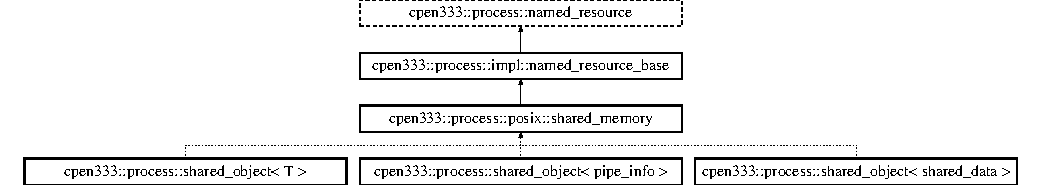
\includegraphics[height=2.488889cm]{classcpen333_1_1process_1_1posix_1_1shared__memory}
\end{center}
\end{figure}
\subsection*{Public Types}
\begin{DoxyCompactItemize}
\item 
\mbox{\Hypertarget{classcpen333_1_1process_1_1posix_1_1shared__memory_a4bec0d0093c8bcfa3283a5da8ef1fc78}\label{classcpen333_1_1process_1_1posix_1_1shared__memory_a4bec0d0093c8bcfa3283a5da8ef1fc78}} 
using \hyperlink{classcpen333_1_1process_1_1posix_1_1shared__memory_a4bec0d0093c8bcfa3283a5da8ef1fc78}{native\+\_\+handle\+\_\+type} = int
\begin{DoxyCompactList}\small\item\em Alias to native handle for shared memory. \end{DoxyCompactList}\end{DoxyCompactItemize}
\subsection*{Public Member Functions}
\begin{DoxyCompactItemize}
\item 
\hyperlink{classcpen333_1_1process_1_1posix_1_1shared__memory_a8a8f0918f8e132e0369c6e9ca9aa6bb6}{shared\+\_\+memory} (const std\+::string \&\hyperlink{classcpen333_1_1process_1_1impl_1_1named__resource__base_a53986a0a1dd26a3602b842c45613b79d}{name}, size\+\_\+t size, bool readonly=false)
\begin{DoxyCompactList}\small\item\em Constructs or connects to a block of shared memory. \end{DoxyCompactList}\item 
\mbox{\Hypertarget{classcpen333_1_1process_1_1posix_1_1shared__memory_a618389d509320111d7aef051fbd32c07}\label{classcpen333_1_1process_1_1posix_1_1shared__memory_a618389d509320111d7aef051fbd32c07}} 
\hyperlink{classcpen333_1_1process_1_1posix_1_1shared__memory_a618389d509320111d7aef051fbd32c07}{$\sim$shared\+\_\+memory} ()
\begin{DoxyCompactList}\small\item\em Destructor, unmaps this instance of the shared memory block (but does not unmap memory from other users) \end{DoxyCompactList}\item 
void $\ast$ \hyperlink{classcpen333_1_1process_1_1posix_1_1shared__memory_ae97ceec75dc83d43a995daac4769504d}{get} (size\+\_\+t offset=0)
\begin{DoxyCompactList}\small\item\em Pointer to memory at a particular offset from the block. \end{DoxyCompactList}\item 
uint8\+\_\+t \& \hyperlink{classcpen333_1_1process_1_1posix_1_1shared__memory_a832b82cb6ab398e814418b516dba2dd9}{operator\mbox{[}$\,$\mbox{]}} (size\+\_\+t offset)
\begin{DoxyCompactList}\small\item\em Byte access, by reference. \end{DoxyCompactList}\item 
{\footnotesize template$<$typename T $>$ }\\T $\ast$ \hyperlink{classcpen333_1_1process_1_1posix_1_1shared__memory_a09582d7b2863aebbbd74d2f32d0b1af8}{get} (size\+\_\+t offset)
\begin{DoxyCompactList}\small\item\em Retrieves a pointer to an object of specified type starting at a particular offset. \end{DoxyCompactList}\item 
{\footnotesize template$<$typename T $>$ }\\T $\ast$ \hyperlink{classcpen333_1_1process_1_1posix_1_1shared__memory_a705beedc2e0b3bde2e044fe742f641ea}{get} ()
\begin{DoxyCompactList}\small\item\em Retrieves a pointer to the underlying memory, cast to a specified type. \end{DoxyCompactList}\item 
bool \hyperlink{classcpen333_1_1process_1_1posix_1_1shared__memory_a3b6d67a41cfaca3712d87958682d8bbe}{unlink} ()
\begin{DoxyCompactList}\small\item\em Detaches the name from the named resource. \end{DoxyCompactList}\item 
\hyperlink{classcpen333_1_1process_1_1posix_1_1shared__memory_a4bec0d0093c8bcfa3283a5da8ef1fc78}{native\+\_\+handle\+\_\+type} \hyperlink{classcpen333_1_1process_1_1posix_1_1shared__memory_ac0dd258666565953b8c6bdbde7aa871f}{native\+\_\+handle} ()
\begin{DoxyCompactList}\small\item\em Native handle to underlying shared memory block. \end{DoxyCompactList}\end{DoxyCompactItemize}
\subsection*{Static Public Member Functions}
\begin{DoxyCompactItemize}
\item 
static bool \hyperlink{classcpen333_1_1process_1_1posix_1_1shared__memory_a68a9ecfafed3c939bc9c38edee71d584}{unlink} (const std\+::string \&\hyperlink{classcpen333_1_1process_1_1impl_1_1named__resource__base_a53986a0a1dd26a3602b842c45613b79d}{name})
\begin{DoxyCompactList}\small\item\em Unlinks the name without needing to create a resource. \end{DoxyCompactList}\end{DoxyCompactItemize}
\subsection*{Additional Inherited Members}


\subsection{Detailed Description}
Inter-\/process shared memory implementation. 

Creates and shares a block of memory between threads/processes, accessible using a unique name. The block of memory is mapped to D\+I\+F\+F\+E\+R\+E\+NT address spaces on each process. This is essentially a memory-\/mapped file.

This shared memory has K\+E\+R\+N\+EL P\+E\+R\+S\+I\+S\+T\+E\+N\+CE, meaning if not \hyperlink{classcpen333_1_1process_1_1posix_1_1shared__memory_a3b6d67a41cfaca3712d87958682d8bbe}{unlink()}-\/ed, will continue to exist in its current state until the system is shut down (persisting beyond the life of the initiating program) 

\subsection{Constructor \& Destructor Documentation}
\mbox{\Hypertarget{classcpen333_1_1process_1_1posix_1_1shared__memory_a8a8f0918f8e132e0369c6e9ca9aa6bb6}\label{classcpen333_1_1process_1_1posix_1_1shared__memory_a8a8f0918f8e132e0369c6e9ca9aa6bb6}} 
\index{cpen333\+::process\+::posix\+::shared\+\_\+memory@{cpen333\+::process\+::posix\+::shared\+\_\+memory}!shared\+\_\+memory@{shared\+\_\+memory}}
\index{shared\+\_\+memory@{shared\+\_\+memory}!cpen333\+::process\+::posix\+::shared\+\_\+memory@{cpen333\+::process\+::posix\+::shared\+\_\+memory}}
\subsubsection{\texorpdfstring{shared\+\_\+memory()}{shared\_memory()}}
{\footnotesize\ttfamily cpen333\+::process\+::posix\+::shared\+\_\+memory\+::shared\+\_\+memory (\begin{DoxyParamCaption}\item[{const std\+::string \&}]{name,  }\item[{size\+\_\+t}]{size,  }\item[{bool}]{readonly = {\ttfamily false} }\end{DoxyParamCaption})\hspace{0.3cm}{\ttfamily [inline]}}



Constructs or connects to a block of shared memory. 


\begin{DoxyParams}{Parameters}
{\em name} & identifier for creating or connecting to an existing inter-\/process shared memory block \\
\hline
{\em size} & if creating, the size of the memory block. This size should be consistent between users \\
\hline
{\em readonly} & whether or not to map the memory as read-\/only \\
\hline
\end{DoxyParams}


\subsection{Member Function Documentation}
\mbox{\Hypertarget{classcpen333_1_1process_1_1posix_1_1shared__memory_ae97ceec75dc83d43a995daac4769504d}\label{classcpen333_1_1process_1_1posix_1_1shared__memory_ae97ceec75dc83d43a995daac4769504d}} 
\index{cpen333\+::process\+::posix\+::shared\+\_\+memory@{cpen333\+::process\+::posix\+::shared\+\_\+memory}!get@{get}}
\index{get@{get}!cpen333\+::process\+::posix\+::shared\+\_\+memory@{cpen333\+::process\+::posix\+::shared\+\_\+memory}}
\subsubsection{\texorpdfstring{get()}{get()}\hspace{0.1cm}{\footnotesize\ttfamily [1/3]}}
{\footnotesize\ttfamily void$\ast$ cpen333\+::process\+::posix\+::shared\+\_\+memory\+::get (\begin{DoxyParamCaption}\item[{size\+\_\+t}]{offset = {\ttfamily 0} }\end{DoxyParamCaption})\hspace{0.3cm}{\ttfamily [inline]}}



Pointer to memory at a particular offset from the block. 


\begin{DoxyParams}{Parameters}
{\em offset} & memory offset (in bytes) \\
\hline
\end{DoxyParams}
\begin{DoxyReturn}{Returns}
pointer to memory offset 
\end{DoxyReturn}
\mbox{\Hypertarget{classcpen333_1_1process_1_1posix_1_1shared__memory_a09582d7b2863aebbbd74d2f32d0b1af8}\label{classcpen333_1_1process_1_1posix_1_1shared__memory_a09582d7b2863aebbbd74d2f32d0b1af8}} 
\index{cpen333\+::process\+::posix\+::shared\+\_\+memory@{cpen333\+::process\+::posix\+::shared\+\_\+memory}!get@{get}}
\index{get@{get}!cpen333\+::process\+::posix\+::shared\+\_\+memory@{cpen333\+::process\+::posix\+::shared\+\_\+memory}}
\subsubsection{\texorpdfstring{get()}{get()}\hspace{0.1cm}{\footnotesize\ttfamily [2/3]}}
{\footnotesize\ttfamily template$<$typename T $>$ \\
T$\ast$ cpen333\+::process\+::posix\+::shared\+\_\+memory\+::get (\begin{DoxyParamCaption}\item[{size\+\_\+t}]{offset }\end{DoxyParamCaption})\hspace{0.3cm}{\ttfamily [inline]}}



Retrieves a pointer to an object of specified type starting at a particular offset. 


\begin{DoxyTemplParams}{Template Parameters}
{\em T} & type of pointer to return \\
\hline
\end{DoxyTemplParams}

\begin{DoxyParams}{Parameters}
{\em offset} & memory offset (in bytes) \\
\hline
\end{DoxyParams}
\begin{DoxyReturn}{Returns}
pointer to object 
\end{DoxyReturn}
\mbox{\Hypertarget{classcpen333_1_1process_1_1posix_1_1shared__memory_a705beedc2e0b3bde2e044fe742f641ea}\label{classcpen333_1_1process_1_1posix_1_1shared__memory_a705beedc2e0b3bde2e044fe742f641ea}} 
\index{cpen333\+::process\+::posix\+::shared\+\_\+memory@{cpen333\+::process\+::posix\+::shared\+\_\+memory}!get@{get}}
\index{get@{get}!cpen333\+::process\+::posix\+::shared\+\_\+memory@{cpen333\+::process\+::posix\+::shared\+\_\+memory}}
\subsubsection{\texorpdfstring{get()}{get()}\hspace{0.1cm}{\footnotesize\ttfamily [3/3]}}
{\footnotesize\ttfamily template$<$typename T $>$ \\
T$\ast$ cpen333\+::process\+::posix\+::shared\+\_\+memory\+::get (\begin{DoxyParamCaption}{ }\end{DoxyParamCaption})\hspace{0.3cm}{\ttfamily [inline]}}



Retrieves a pointer to the underlying memory, cast to a specified type. 


\begin{DoxyTemplParams}{Template Parameters}
{\em T} & type of pointer to return \\
\hline
\end{DoxyTemplParams}
\begin{DoxyReturn}{Returns}
pointer to object 
\end{DoxyReturn}
\mbox{\Hypertarget{classcpen333_1_1process_1_1posix_1_1shared__memory_ac0dd258666565953b8c6bdbde7aa871f}\label{classcpen333_1_1process_1_1posix_1_1shared__memory_ac0dd258666565953b8c6bdbde7aa871f}} 
\index{cpen333\+::process\+::posix\+::shared\+\_\+memory@{cpen333\+::process\+::posix\+::shared\+\_\+memory}!native\+\_\+handle@{native\+\_\+handle}}
\index{native\+\_\+handle@{native\+\_\+handle}!cpen333\+::process\+::posix\+::shared\+\_\+memory@{cpen333\+::process\+::posix\+::shared\+\_\+memory}}
\subsubsection{\texorpdfstring{native\+\_\+handle()}{native\_handle()}}
{\footnotesize\ttfamily \hyperlink{classcpen333_1_1process_1_1posix_1_1shared__memory_a4bec0d0093c8bcfa3283a5da8ef1fc78}{native\+\_\+handle\+\_\+type} cpen333\+::process\+::posix\+::shared\+\_\+memory\+::native\+\_\+handle (\begin{DoxyParamCaption}{ }\end{DoxyParamCaption})\hspace{0.3cm}{\ttfamily [inline]}}



Native handle to underlying shared memory block. 

On P\+O\+S\+IX systems, this is a P\+O\+S\+IX shm id

\begin{DoxyReturn}{Returns}
native handle to shared memory block 
\end{DoxyReturn}
\mbox{\Hypertarget{classcpen333_1_1process_1_1posix_1_1shared__memory_a832b82cb6ab398e814418b516dba2dd9}\label{classcpen333_1_1process_1_1posix_1_1shared__memory_a832b82cb6ab398e814418b516dba2dd9}} 
\index{cpen333\+::process\+::posix\+::shared\+\_\+memory@{cpen333\+::process\+::posix\+::shared\+\_\+memory}!operator\mbox{[}\mbox{]}@{operator[]}}
\index{operator\mbox{[}\mbox{]}@{operator[]}!cpen333\+::process\+::posix\+::shared\+\_\+memory@{cpen333\+::process\+::posix\+::shared\+\_\+memory}}
\subsubsection{\texorpdfstring{operator[]()}{operator[]()}}
{\footnotesize\ttfamily uint8\+\_\+t\& cpen333\+::process\+::posix\+::shared\+\_\+memory\+::operator\mbox{[}$\,$\mbox{]} (\begin{DoxyParamCaption}\item[{size\+\_\+t}]{offset }\end{DoxyParamCaption})\hspace{0.3cm}{\ttfamily [inline]}}



Byte access, by reference. 


\begin{DoxyParams}{Parameters}
{\em offset} & memory offset (in bytes) \\
\hline
\end{DoxyParams}
\begin{DoxyReturn}{Returns}
byte at particular offset 
\end{DoxyReturn}
\mbox{\Hypertarget{classcpen333_1_1process_1_1posix_1_1shared__memory_a3b6d67a41cfaca3712d87958682d8bbe}\label{classcpen333_1_1process_1_1posix_1_1shared__memory_a3b6d67a41cfaca3712d87958682d8bbe}} 
\index{cpen333\+::process\+::posix\+::shared\+\_\+memory@{cpen333\+::process\+::posix\+::shared\+\_\+memory}!unlink@{unlink}}
\index{unlink@{unlink}!cpen333\+::process\+::posix\+::shared\+\_\+memory@{cpen333\+::process\+::posix\+::shared\+\_\+memory}}
\subsubsection{\texorpdfstring{unlink()}{unlink()}\hspace{0.1cm}{\footnotesize\ttfamily [1/2]}}
{\footnotesize\ttfamily bool cpen333\+::process\+::posix\+::shared\+\_\+memory\+::unlink (\begin{DoxyParamCaption}{ }\end{DoxyParamCaption})\hspace{0.3cm}{\ttfamily [inline]}, {\ttfamily [virtual]}}



Detaches the name from the named resource. 

On P\+O\+S\+IX systems, named resources will persist beyond the lifetime of any process that uses them as long as the name has not been unlinked (or until the system is rebooted). Calling {\ttfamily unlink} will detach the name, allowing the resource to be freed once all current users have exited.

\begin{DoxyReturn}{Returns}
{\ttfamily true} if unlink is successful, {\ttfamily false} if unlinking is not supported or if an error has occurred. 
\end{DoxyReturn}


Implements \hyperlink{classcpen333_1_1process_1_1impl_1_1named__resource__base_ae4033f82dfd068b917a9bca57d3a0c45}{cpen333\+::process\+::impl\+::named\+\_\+resource\+\_\+base}.



Reimplemented in \hyperlink{classcpen333_1_1process_1_1shared__object_aa5b43829da5bd2376927e6285745211c}{cpen333\+::process\+::shared\+\_\+object$<$ T $>$}, \hyperlink{classcpen333_1_1process_1_1shared__object_aa5b43829da5bd2376927e6285745211c}{cpen333\+::process\+::shared\+\_\+object$<$ pipe\+\_\+info $>$}, and \hyperlink{classcpen333_1_1process_1_1shared__object_aa5b43829da5bd2376927e6285745211c}{cpen333\+::process\+::shared\+\_\+object$<$ shared\+\_\+data $>$}.

\mbox{\Hypertarget{classcpen333_1_1process_1_1posix_1_1shared__memory_a68a9ecfafed3c939bc9c38edee71d584}\label{classcpen333_1_1process_1_1posix_1_1shared__memory_a68a9ecfafed3c939bc9c38edee71d584}} 
\index{cpen333\+::process\+::posix\+::shared\+\_\+memory@{cpen333\+::process\+::posix\+::shared\+\_\+memory}!unlink@{unlink}}
\index{unlink@{unlink}!cpen333\+::process\+::posix\+::shared\+\_\+memory@{cpen333\+::process\+::posix\+::shared\+\_\+memory}}
\subsubsection{\texorpdfstring{unlink()}{unlink()}\hspace{0.1cm}{\footnotesize\ttfamily [2/2]}}
{\footnotesize\ttfamily static bool cpen333\+::process\+::posix\+::shared\+\_\+memory\+::unlink (\begin{DoxyParamCaption}\item[{const std\+::string \&}]{name }\end{DoxyParamCaption})\hspace{0.3cm}{\ttfamily [inline]}, {\ttfamily [static]}}



Unlinks the name without needing to create a resource. 

Implementers should also provide a static method for unlinking. The purpose is mainly for clean-\/up of existing resources.


\begin{DoxyParams}{Parameters}
{\em name} & desired resource name \\
\hline
\end{DoxyParams}
\begin{DoxyReturn}{Returns}
{\ttfamily true} if unlink successful, {\ttfamily false} if not successful or not supported 
\end{DoxyReturn}


The documentation for this class was generated from the following file\+:\begin{DoxyCompactItemize}
\item 
D\+:/school/teaching/\+C\+P\+E\+N333/workspace/library/include/cpen333/process/impl/posix/\hyperlink{impl_2posix_2shared__memory_8h}{shared\+\_\+memory.\+h}\end{DoxyCompactItemize}

\hypertarget{classcpen333_1_1process_1_1windows_1_1shared__memory}{}\section{cpen333\+:\+:process\+:\+:windows\+:\+:shared\+\_\+memory Class Reference}
\label{classcpen333_1_1process_1_1windows_1_1shared__memory}\index{cpen333\+::process\+::windows\+::shared\+\_\+memory@{cpen333\+::process\+::windows\+::shared\+\_\+memory}}


Inter-\/process shared memory implementation.  




{\ttfamily \#include $<$shared\+\_\+memory.\+h$>$}

Inheritance diagram for cpen333\+:\+:process\+:\+:windows\+:\+:shared\+\_\+memory\+:\begin{figure}[H]
\begin{center}
\leavevmode
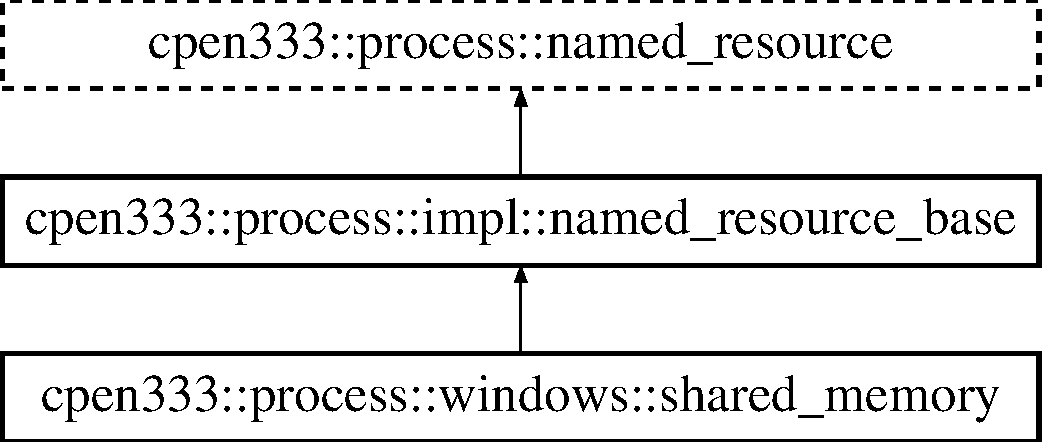
\includegraphics[height=3.000000cm]{classcpen333_1_1process_1_1windows_1_1shared__memory}
\end{center}
\end{figure}
\subsection*{Public Types}
\begin{DoxyCompactItemize}
\item 
\mbox{\Hypertarget{classcpen333_1_1process_1_1windows_1_1shared__memory_a4a2507680675101666846b0975fa6899}\label{classcpen333_1_1process_1_1windows_1_1shared__memory_a4a2507680675101666846b0975fa6899}} 
typedef H\+A\+N\+D\+LE \hyperlink{classcpen333_1_1process_1_1windows_1_1shared__memory_a4a2507680675101666846b0975fa6899}{native\+\_\+handle\+\_\+type}
\begin{DoxyCompactList}\small\item\em Alias to native handle for shared memory. \end{DoxyCompactList}\end{DoxyCompactItemize}
\subsection*{Public Member Functions}
\begin{DoxyCompactItemize}
\item 
\hyperlink{classcpen333_1_1process_1_1windows_1_1shared__memory_a3a2044ba961f9fc394e166273a3efa20}{shared\+\_\+memory} (const std\+::string \&\hyperlink{classcpen333_1_1process_1_1impl_1_1named__resource__base_a53986a0a1dd26a3602b842c45613b79d}{name}, size\+\_\+t size, bool readonly=false)
\begin{DoxyCompactList}\small\item\em Constructs or connects to a block of shared memory. \end{DoxyCompactList}\item 
\hyperlink{classcpen333_1_1process_1_1windows_1_1shared__memory_a6355690147ae22f25d4bceed8ad63011}{$\sim$shared\+\_\+memory} ()
\begin{DoxyCompactList}\small\item\em Destructor, unmaps this instance of the shared memory block (but does not unmap memory from other users) \end{DoxyCompactList}\item 
void $\ast$ \hyperlink{classcpen333_1_1process_1_1windows_1_1shared__memory_a3bbd718728dc2fa2fbe4058b8a207594}{get} (size\+\_\+t offset=0)
\begin{DoxyCompactList}\small\item\em Pointer to memory at a particular offset from the block. \end{DoxyCompactList}\item 
uint8\+\_\+t \& \hyperlink{classcpen333_1_1process_1_1windows_1_1shared__memory_a931719bdcc1558973d6fcb7a79f52f22}{operator\mbox{[}$\,$\mbox{]}} (size\+\_\+t offset)
\begin{DoxyCompactList}\small\item\em Byte access, by reference. \end{DoxyCompactList}\item 
{\footnotesize template$<$typename T $>$ }\\T $\ast$ \hyperlink{classcpen333_1_1process_1_1windows_1_1shared__memory_a2f2fa53c705df531b6126ed2da84c347}{get} (size\+\_\+t offset)
\begin{DoxyCompactList}\small\item\em Pointer to memory at a particular offset from the block. \end{DoxyCompactList}\item 
{\footnotesize template$<$typename T $>$ }\\T $\ast$ \hyperlink{classcpen333_1_1process_1_1windows_1_1shared__memory_a3986cdc917b26ab1ab608f59270a47c5}{get} ()
\begin{DoxyCompactList}\small\item\em Retrieves a pointer to the underlying memory, cast to a specified type. \end{DoxyCompactList}\item 
\hyperlink{classcpen333_1_1process_1_1windows_1_1shared__memory_a4a2507680675101666846b0975fa6899}{native\+\_\+handle\+\_\+type} \hyperlink{classcpen333_1_1process_1_1windows_1_1shared__memory_a1827dd03341d7c6afcc02cf078f54e32}{native\+\_\+handle} ()
\begin{DoxyCompactList}\small\item\em Native handle to underlying shared memory block. \end{DoxyCompactList}\item 
bool \hyperlink{classcpen333_1_1process_1_1windows_1_1shared__memory_aa6efdc9a3e1310ea69ecc48aeb41286c}{unlink} ()
\begin{DoxyCompactList}\small\item\em Detaches the name from the named resource. \end{DoxyCompactList}\end{DoxyCompactItemize}
\subsection*{Static Public Member Functions}
\begin{DoxyCompactItemize}
\item 
static bool \hyperlink{classcpen333_1_1process_1_1windows_1_1shared__memory_a99c4766a9995a97595bba1550256f1c9}{unlink} (const std\+::string \&\hyperlink{classcpen333_1_1process_1_1impl_1_1named__resource__base_a53986a0a1dd26a3602b842c45613b79d}{name})
\begin{DoxyCompactList}\small\item\em Unlinks the name without needing to create a resource. \end{DoxyCompactList}\end{DoxyCompactItemize}
\subsection*{Additional Inherited Members}


\subsection{Detailed Description}
Inter-\/process shared memory implementation. 

Creates and shares a block of memory between threads/processes, accessible using a unique name. The block of memory is mapped to D\+I\+F\+F\+E\+R\+E\+NT address spaces on each process. This is essentially a memory-\/mapped file.

This shared memory has U\+S\+A\+GE P\+E\+R\+S\+I\+S\+T\+E\+N\+CE, meaning the mutex will continue to exist as long as at least one process/thread is holding a reference to it. 

\subsection{Constructor \& Destructor Documentation}
\mbox{\Hypertarget{classcpen333_1_1process_1_1windows_1_1shared__memory_a3a2044ba961f9fc394e166273a3efa20}\label{classcpen333_1_1process_1_1windows_1_1shared__memory_a3a2044ba961f9fc394e166273a3efa20}} 
\index{cpen333\+::process\+::windows\+::shared\+\_\+memory@{cpen333\+::process\+::windows\+::shared\+\_\+memory}!shared\+\_\+memory@{shared\+\_\+memory}}
\index{shared\+\_\+memory@{shared\+\_\+memory}!cpen333\+::process\+::windows\+::shared\+\_\+memory@{cpen333\+::process\+::windows\+::shared\+\_\+memory}}
\subsubsection{\texorpdfstring{shared\+\_\+memory()}{shared\_memory()}}
{\footnotesize\ttfamily cpen333\+::process\+::windows\+::shared\+\_\+memory\+::shared\+\_\+memory (\begin{DoxyParamCaption}\item[{const std\+::string \&}]{name,  }\item[{size\+\_\+t}]{size,  }\item[{bool}]{readonly = {\ttfamily false} }\end{DoxyParamCaption})\hspace{0.3cm}{\ttfamily [inline]}}



Constructs or connects to a block of shared memory. 


\begin{DoxyParams}{Parameters}
{\em name} & identifier for creating or connecting to an existing inter-\/process shared memory block \\
\hline
{\em size} & if creating, the size of the memory block. This size should be consistent between users \\
\hline
{\em readonly} & whether or not to map the memory as read-\/only \\
\hline
\end{DoxyParams}
\mbox{\Hypertarget{classcpen333_1_1process_1_1windows_1_1shared__memory_a6355690147ae22f25d4bceed8ad63011}\label{classcpen333_1_1process_1_1windows_1_1shared__memory_a6355690147ae22f25d4bceed8ad63011}} 
\index{cpen333\+::process\+::windows\+::shared\+\_\+memory@{cpen333\+::process\+::windows\+::shared\+\_\+memory}!````~shared\+\_\+memory@{$\sim$shared\+\_\+memory}}
\index{````~shared\+\_\+memory@{$\sim$shared\+\_\+memory}!cpen333\+::process\+::windows\+::shared\+\_\+memory@{cpen333\+::process\+::windows\+::shared\+\_\+memory}}
\subsubsection{\texorpdfstring{$\sim$shared\+\_\+memory()}{~shared\_memory()}}
{\footnotesize\ttfamily cpen333\+::process\+::windows\+::shared\+\_\+memory\+::$\sim$shared\+\_\+memory (\begin{DoxyParamCaption}{ }\end{DoxyParamCaption})\hspace{0.3cm}{\ttfamily [inline]}}



Destructor, unmaps this instance of the shared memory block (but does not unmap memory from other users) 



\subsection{Member Function Documentation}
\mbox{\Hypertarget{classcpen333_1_1process_1_1windows_1_1shared__memory_a3bbd718728dc2fa2fbe4058b8a207594}\label{classcpen333_1_1process_1_1windows_1_1shared__memory_a3bbd718728dc2fa2fbe4058b8a207594}} 
\index{cpen333\+::process\+::windows\+::shared\+\_\+memory@{cpen333\+::process\+::windows\+::shared\+\_\+memory}!get@{get}}
\index{get@{get}!cpen333\+::process\+::windows\+::shared\+\_\+memory@{cpen333\+::process\+::windows\+::shared\+\_\+memory}}
\subsubsection{\texorpdfstring{get()}{get()}\hspace{0.1cm}{\footnotesize\ttfamily [1/3]}}
{\footnotesize\ttfamily void$\ast$ cpen333\+::process\+::windows\+::shared\+\_\+memory\+::get (\begin{DoxyParamCaption}\item[{size\+\_\+t}]{offset = {\ttfamily 0} }\end{DoxyParamCaption})\hspace{0.3cm}{\ttfamily [inline]}}



Pointer to memory at a particular offset from the block. 


\begin{DoxyParams}{Parameters}
{\em offset} & memory offset (in bytes) \\
\hline
\end{DoxyParams}
\begin{DoxyReturn}{Returns}
pointer to memory offset 
\end{DoxyReturn}
\mbox{\Hypertarget{classcpen333_1_1process_1_1windows_1_1shared__memory_a2f2fa53c705df531b6126ed2da84c347}\label{classcpen333_1_1process_1_1windows_1_1shared__memory_a2f2fa53c705df531b6126ed2da84c347}} 
\index{cpen333\+::process\+::windows\+::shared\+\_\+memory@{cpen333\+::process\+::windows\+::shared\+\_\+memory}!get@{get}}
\index{get@{get}!cpen333\+::process\+::windows\+::shared\+\_\+memory@{cpen333\+::process\+::windows\+::shared\+\_\+memory}}
\subsubsection{\texorpdfstring{get()}{get()}\hspace{0.1cm}{\footnotesize\ttfamily [2/3]}}
{\footnotesize\ttfamily template$<$typename T $>$ \\
T$\ast$ cpen333\+::process\+::windows\+::shared\+\_\+memory\+::get (\begin{DoxyParamCaption}\item[{size\+\_\+t}]{offset }\end{DoxyParamCaption})\hspace{0.3cm}{\ttfamily [inline]}}



Pointer to memory at a particular offset from the block. 


\begin{DoxyParams}{Parameters}
{\em offset} & memory offset (in bytes) \\
\hline
\end{DoxyParams}
\begin{DoxyReturn}{Returns}
pointer to memory offset 
\end{DoxyReturn}
\mbox{\Hypertarget{classcpen333_1_1process_1_1windows_1_1shared__memory_a3986cdc917b26ab1ab608f59270a47c5}\label{classcpen333_1_1process_1_1windows_1_1shared__memory_a3986cdc917b26ab1ab608f59270a47c5}} 
\index{cpen333\+::process\+::windows\+::shared\+\_\+memory@{cpen333\+::process\+::windows\+::shared\+\_\+memory}!get@{get}}
\index{get@{get}!cpen333\+::process\+::windows\+::shared\+\_\+memory@{cpen333\+::process\+::windows\+::shared\+\_\+memory}}
\subsubsection{\texorpdfstring{get()}{get()}\hspace{0.1cm}{\footnotesize\ttfamily [3/3]}}
{\footnotesize\ttfamily template$<$typename T $>$ \\
T$\ast$ cpen333\+::process\+::windows\+::shared\+\_\+memory\+::get (\begin{DoxyParamCaption}{ }\end{DoxyParamCaption})\hspace{0.3cm}{\ttfamily [inline]}}



Retrieves a pointer to the underlying memory, cast to a specified type. 


\begin{DoxyTemplParams}{Template Parameters}
{\em T} & type of pointer to return \\
\hline
\end{DoxyTemplParams}
\begin{DoxyReturn}{Returns}
pointer to object 
\end{DoxyReturn}
\mbox{\Hypertarget{classcpen333_1_1process_1_1windows_1_1shared__memory_a1827dd03341d7c6afcc02cf078f54e32}\label{classcpen333_1_1process_1_1windows_1_1shared__memory_a1827dd03341d7c6afcc02cf078f54e32}} 
\index{cpen333\+::process\+::windows\+::shared\+\_\+memory@{cpen333\+::process\+::windows\+::shared\+\_\+memory}!native\+\_\+handle@{native\+\_\+handle}}
\index{native\+\_\+handle@{native\+\_\+handle}!cpen333\+::process\+::windows\+::shared\+\_\+memory@{cpen333\+::process\+::windows\+::shared\+\_\+memory}}
\subsubsection{\texorpdfstring{native\+\_\+handle()}{native\_handle()}}
{\footnotesize\ttfamily \hyperlink{classcpen333_1_1process_1_1windows_1_1shared__memory_a4a2507680675101666846b0975fa6899}{native\+\_\+handle\+\_\+type} cpen333\+::process\+::windows\+::shared\+\_\+memory\+::native\+\_\+handle (\begin{DoxyParamCaption}{ }\end{DoxyParamCaption})\hspace{0.3cm}{\ttfamily [inline]}}



Native handle to underlying shared memory block. 

On Windows systems, this is a Windows H\+A\+N\+D\+LE to the memory-\/mapped file mapping

\begin{DoxyReturn}{Returns}
native handle to shared memory block 
\end{DoxyReturn}
\mbox{\Hypertarget{classcpen333_1_1process_1_1windows_1_1shared__memory_a931719bdcc1558973d6fcb7a79f52f22}\label{classcpen333_1_1process_1_1windows_1_1shared__memory_a931719bdcc1558973d6fcb7a79f52f22}} 
\index{cpen333\+::process\+::windows\+::shared\+\_\+memory@{cpen333\+::process\+::windows\+::shared\+\_\+memory}!operator\mbox{[}\mbox{]}@{operator[]}}
\index{operator\mbox{[}\mbox{]}@{operator[]}!cpen333\+::process\+::windows\+::shared\+\_\+memory@{cpen333\+::process\+::windows\+::shared\+\_\+memory}}
\subsubsection{\texorpdfstring{operator[]()}{operator[]()}}
{\footnotesize\ttfamily uint8\+\_\+t\& cpen333\+::process\+::windows\+::shared\+\_\+memory\+::operator\mbox{[}$\,$\mbox{]} (\begin{DoxyParamCaption}\item[{size\+\_\+t}]{offset }\end{DoxyParamCaption})\hspace{0.3cm}{\ttfamily [inline]}}



Byte access, by reference. 


\begin{DoxyParams}{Parameters}
{\em offset} & memory offset (in bytes) \\
\hline
\end{DoxyParams}
\begin{DoxyReturn}{Returns}
byte at particular offset 
\end{DoxyReturn}
\mbox{\Hypertarget{classcpen333_1_1process_1_1windows_1_1shared__memory_aa6efdc9a3e1310ea69ecc48aeb41286c}\label{classcpen333_1_1process_1_1windows_1_1shared__memory_aa6efdc9a3e1310ea69ecc48aeb41286c}} 
\index{cpen333\+::process\+::windows\+::shared\+\_\+memory@{cpen333\+::process\+::windows\+::shared\+\_\+memory}!unlink@{unlink}}
\index{unlink@{unlink}!cpen333\+::process\+::windows\+::shared\+\_\+memory@{cpen333\+::process\+::windows\+::shared\+\_\+memory}}
\subsubsection{\texorpdfstring{unlink()}{unlink()}\hspace{0.1cm}{\footnotesize\ttfamily [1/2]}}
{\footnotesize\ttfamily bool cpen333\+::process\+::windows\+::shared\+\_\+memory\+::unlink (\begin{DoxyParamCaption}{ }\end{DoxyParamCaption})\hspace{0.3cm}{\ttfamily [inline]}, {\ttfamily [virtual]}}



Detaches the name from the named resource. 

On P\+O\+S\+IX systems, named resources will persist beyond the lifetime of any process that uses them as long as the name has not been unlinked (or until the system is rebooted). Calling {\ttfamily unlink} will detach the name, allowing the resource to be freed once all current users have exited.

\begin{DoxyReturn}{Returns}
{\ttfamily true} if unlink is successful, {\ttfamily false} if unlinking is not supported or if an error has occurred. 
\end{DoxyReturn}


Implements \hyperlink{classcpen333_1_1process_1_1impl_1_1named__resource__base_ae4033f82dfd068b917a9bca57d3a0c45}{cpen333\+::process\+::impl\+::named\+\_\+resource\+\_\+base}.

\mbox{\Hypertarget{classcpen333_1_1process_1_1windows_1_1shared__memory_a99c4766a9995a97595bba1550256f1c9}\label{classcpen333_1_1process_1_1windows_1_1shared__memory_a99c4766a9995a97595bba1550256f1c9}} 
\index{cpen333\+::process\+::windows\+::shared\+\_\+memory@{cpen333\+::process\+::windows\+::shared\+\_\+memory}!unlink@{unlink}}
\index{unlink@{unlink}!cpen333\+::process\+::windows\+::shared\+\_\+memory@{cpen333\+::process\+::windows\+::shared\+\_\+memory}}
\subsubsection{\texorpdfstring{unlink()}{unlink()}\hspace{0.1cm}{\footnotesize\ttfamily [2/2]}}
{\footnotesize\ttfamily static bool cpen333\+::process\+::windows\+::shared\+\_\+memory\+::unlink (\begin{DoxyParamCaption}\item[{const std\+::string \&}]{name }\end{DoxyParamCaption})\hspace{0.3cm}{\ttfamily [inline]}, {\ttfamily [static]}}



Unlinks the name without needing to create a resource. 

Implementers should also provide a static method for unlinking. The purpose is mainly for clean-\/up of existing resources.


\begin{DoxyParams}{Parameters}
{\em name} & desired resource name \\
\hline
\end{DoxyParams}
\begin{DoxyReturn}{Returns}
{\ttfamily true} if unlink successful, {\ttfamily false} if not successful or not supported 
\end{DoxyReturn}


The documentation for this class was generated from the following file\+:\begin{DoxyCompactItemize}
\item 
D\+:/school/teaching/\+C\+P\+E\+N333/workspace/library/include/cpen333/process/impl/windows/\hyperlink{impl_2windows_2shared__memory_8h}{shared\+\_\+memory.\+h}\end{DoxyCompactItemize}

\input{classcpen333_1_1process_1_1shared__mutex}
\input{classcpen333_1_1process_1_1impl_1_1shared__mutex__exclusive}
\input{classcpen333_1_1thread_1_1impl_1_1shared__mutex__exclusive}
\input{classcpen333_1_1thread_1_1impl_1_1shared__mutex__fair}
\input{classcpen333_1_1process_1_1impl_1_1shared__mutex__fair}
\input{classcpen333_1_1thread_1_1impl_1_1shared__mutex__shared}
\input{classcpen333_1_1process_1_1impl_1_1shared__mutex__shared}
\hypertarget{classcpen333_1_1process_1_1shared__object}{}\section{cpen333\+:\+:process\+:\+:shared\+\_\+object$<$ T $>$ Class Template Reference}
\label{classcpen333_1_1process_1_1shared__object}\index{cpen333\+::process\+::shared\+\_\+object$<$ T $>$@{cpen333\+::process\+::shared\+\_\+object$<$ T $>$}}


Shared memory with a a specific stored type.  




{\ttfamily \#include $<$shared\+\_\+memory.\+h$>$}

Inheritance diagram for cpen333\+:\+:process\+:\+:shared\+\_\+object$<$ T $>$\+:\begin{figure}[H]
\begin{center}
\leavevmode
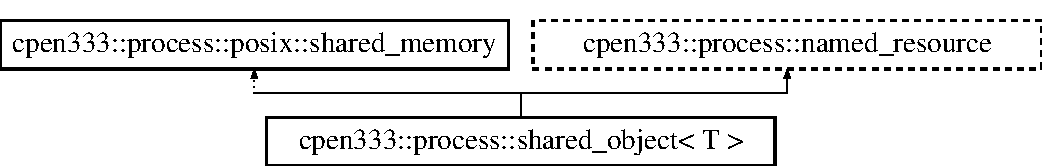
\includegraphics[height=2.000000cm]{classcpen333_1_1process_1_1shared__object}
\end{center}
\end{figure}
\subsection*{Public Member Functions}
\begin{DoxyCompactItemize}
\item 
\hyperlink{classcpen333_1_1process_1_1shared__object_ac8e7c58b5066b058d32e27a7d068f504}{shared\+\_\+object} (const std\+::string \&\hyperlink{classcpen333_1_1process_1_1impl_1_1named__resource__base_a53986a0a1dd26a3602b842c45613b79d}{name}, bool readonly=false)
\begin{DoxyCompactList}\small\item\em Construct shared memory object. \end{DoxyCompactList}\item 
T \& \hyperlink{classcpen333_1_1process_1_1shared__object_ad1ffd4ad5e13a87f27d9253b816b0b9f}{operator$\ast$} ()
\begin{DoxyCompactList}\small\item\em Get a reference to the internal shared memory object. \end{DoxyCompactList}\item 
T $\ast$ \hyperlink{classcpen333_1_1process_1_1shared__object_ad5a71ce94a79904c4ef85c5a5d1f44f9}{operator-\/$>$} ()
\begin{DoxyCompactList}\small\item\em Get a pointer to the underlying shared memory object. \end{DoxyCompactList}\item 
T $\ast$ \hyperlink{classcpen333_1_1process_1_1shared__object_ac6d38c3ca35cfb102905b6e9dbe4b1ce}{get} ()
\begin{DoxyCompactList}\small\item\em Get a pointer to the underlying shared memory object. \end{DoxyCompactList}\item 
bool \hyperlink{classcpen333_1_1process_1_1shared__object_aa5b43829da5bd2376927e6285745211c}{unlink} ()
\begin{DoxyCompactList}\small\item\em Detaches the name from the named resource. \end{DoxyCompactList}\end{DoxyCompactItemize}
\subsection*{Static Public Member Functions}
\begin{DoxyCompactItemize}
\item 
static bool \hyperlink{classcpen333_1_1process_1_1shared__object_a478c2228031b8471b1e729ce78aabd97}{unlink} (const std\+::string \&\hyperlink{classcpen333_1_1process_1_1impl_1_1named__resource__base_a53986a0a1dd26a3602b842c45613b79d}{name})
\begin{DoxyCompactList}\small\item\em Unlinks the name without needing to create a resource. \end{DoxyCompactList}\end{DoxyCompactItemize}


\subsection{Detailed Description}
\subsubsection*{template$<$typename T$>$\newline
class cpen333\+::process\+::shared\+\_\+object$<$ T $>$}

Shared memory with a a specific stored type. 

With typed shared memory, the size of the required memory block is automatically computed, and the data pointer is automatically cast to the correct type in \hyperlink{classcpen333_1_1process_1_1shared__object_ac6d38c3ca35cfb102905b6e9dbe4b1ce}{get()}. Member access operators are also overloaded for convenience so the shared object can be used as if it is a direct pointer to the underlying data.


\begin{DoxyTemplParams}{Template Parameters}
{\em T} & data type \\
\hline
\end{DoxyTemplParams}


\subsection{Constructor \& Destructor Documentation}
\mbox{\Hypertarget{classcpen333_1_1process_1_1shared__object_ac8e7c58b5066b058d32e27a7d068f504}\label{classcpen333_1_1process_1_1shared__object_ac8e7c58b5066b058d32e27a7d068f504}} 
\index{cpen333\+::process\+::shared\+\_\+object@{cpen333\+::process\+::shared\+\_\+object}!shared\+\_\+object@{shared\+\_\+object}}
\index{shared\+\_\+object@{shared\+\_\+object}!cpen333\+::process\+::shared\+\_\+object@{cpen333\+::process\+::shared\+\_\+object}}
\subsubsection{\texorpdfstring{shared\+\_\+object()}{shared\_object()}}
{\footnotesize\ttfamily template$<$typename T$>$ \\
\hyperlink{classcpen333_1_1process_1_1shared__object}{cpen333\+::process\+::shared\+\_\+object}$<$ T $>$\+::\hyperlink{classcpen333_1_1process_1_1shared__object}{shared\+\_\+object} (\begin{DoxyParamCaption}\item[{const std\+::string \&}]{name,  }\item[{bool}]{readonly = {\ttfamily false} }\end{DoxyParamCaption})\hspace{0.3cm}{\ttfamily [inline]}}



Construct shared memory object. 


\begin{DoxyParams}{Parameters}
{\em name} & identifier for creating or connecting to an existing inter-\/process \hyperlink{classcpen333_1_1process_1_1shared__object}{shared\+\_\+object} \\
\hline
{\em readonly} & whether to treat the memory as read-\/only or read-\/write \\
\hline
\end{DoxyParams}


\subsection{Member Function Documentation}
\mbox{\Hypertarget{classcpen333_1_1process_1_1shared__object_ac6d38c3ca35cfb102905b6e9dbe4b1ce}\label{classcpen333_1_1process_1_1shared__object_ac6d38c3ca35cfb102905b6e9dbe4b1ce}} 
\index{cpen333\+::process\+::shared\+\_\+object@{cpen333\+::process\+::shared\+\_\+object}!get@{get}}
\index{get@{get}!cpen333\+::process\+::shared\+\_\+object@{cpen333\+::process\+::shared\+\_\+object}}
\subsubsection{\texorpdfstring{get()}{get()}}
{\footnotesize\ttfamily template$<$typename T$>$ \\
T$\ast$ \hyperlink{classcpen333_1_1process_1_1shared__object}{cpen333\+::process\+::shared\+\_\+object}$<$ T $>$\+::get (\begin{DoxyParamCaption}{ }\end{DoxyParamCaption})\hspace{0.3cm}{\ttfamily [inline]}}



Get a pointer to the underlying shared memory object. 

\begin{DoxyReturn}{Returns}
pointer to shared data object 
\end{DoxyReturn}
\mbox{\Hypertarget{classcpen333_1_1process_1_1shared__object_ad1ffd4ad5e13a87f27d9253b816b0b9f}\label{classcpen333_1_1process_1_1shared__object_ad1ffd4ad5e13a87f27d9253b816b0b9f}} 
\index{cpen333\+::process\+::shared\+\_\+object@{cpen333\+::process\+::shared\+\_\+object}!operator$\ast$@{operator$\ast$}}
\index{operator$\ast$@{operator$\ast$}!cpen333\+::process\+::shared\+\_\+object@{cpen333\+::process\+::shared\+\_\+object}}
\subsubsection{\texorpdfstring{operator$\ast$()}{operator*()}}
{\footnotesize\ttfamily template$<$typename T$>$ \\
T\& \hyperlink{classcpen333_1_1process_1_1shared__object}{cpen333\+::process\+::shared\+\_\+object}$<$ T $>$\+::operator$\ast$ (\begin{DoxyParamCaption}{ }\end{DoxyParamCaption})\hspace{0.3cm}{\ttfamily [inline]}}



Get a reference to the internal shared memory object. 

\begin{DoxyReturn}{Returns}
reference to shared data object 
\end{DoxyReturn}
\mbox{\Hypertarget{classcpen333_1_1process_1_1shared__object_ad5a71ce94a79904c4ef85c5a5d1f44f9}\label{classcpen333_1_1process_1_1shared__object_ad5a71ce94a79904c4ef85c5a5d1f44f9}} 
\index{cpen333\+::process\+::shared\+\_\+object@{cpen333\+::process\+::shared\+\_\+object}!operator-\/$>$@{operator-\/$>$}}
\index{operator-\/$>$@{operator-\/$>$}!cpen333\+::process\+::shared\+\_\+object@{cpen333\+::process\+::shared\+\_\+object}}
\subsubsection{\texorpdfstring{operator-\/$>$()}{operator->()}}
{\footnotesize\ttfamily template$<$typename T$>$ \\
T$\ast$ \hyperlink{classcpen333_1_1process_1_1shared__object}{cpen333\+::process\+::shared\+\_\+object}$<$ T $>$\+::operator-\/$>$ (\begin{DoxyParamCaption}{ }\end{DoxyParamCaption})\hspace{0.3cm}{\ttfamily [inline]}}



Get a pointer to the underlying shared memory object. 

\begin{DoxyReturn}{Returns}
pointer to shared data object 
\end{DoxyReturn}
\mbox{\Hypertarget{classcpen333_1_1process_1_1shared__object_aa5b43829da5bd2376927e6285745211c}\label{classcpen333_1_1process_1_1shared__object_aa5b43829da5bd2376927e6285745211c}} 
\index{cpen333\+::process\+::shared\+\_\+object@{cpen333\+::process\+::shared\+\_\+object}!unlink@{unlink}}
\index{unlink@{unlink}!cpen333\+::process\+::shared\+\_\+object@{cpen333\+::process\+::shared\+\_\+object}}
\subsubsection{\texorpdfstring{unlink()}{unlink()}\hspace{0.1cm}{\footnotesize\ttfamily [1/2]}}
{\footnotesize\ttfamily template$<$typename T$>$ \\
bool \hyperlink{classcpen333_1_1process_1_1shared__object}{cpen333\+::process\+::shared\+\_\+object}$<$ T $>$\+::unlink (\begin{DoxyParamCaption}{ }\end{DoxyParamCaption})\hspace{0.3cm}{\ttfamily [inline]}, {\ttfamily [virtual]}}



Detaches the name from the named resource. 

On P\+O\+S\+IX systems, named resources will persist beyond the lifetime of any process that uses them as long as the name has not been unlinked (or until the system is rebooted). Calling {\ttfamily unlink} will detach the name, allowing the resource to be freed once all current users have exited.

\begin{DoxyReturn}{Returns}
{\ttfamily true} if unlink is successful, {\ttfamily false} if unlinking is not supported or if an error has occurred. 
\end{DoxyReturn}


Reimplemented from \hyperlink{classcpen333_1_1process_1_1posix_1_1shared__memory_a3b6d67a41cfaca3712d87958682d8bbe}{cpen333\+::process\+::posix\+::shared\+\_\+memory}.

\mbox{\Hypertarget{classcpen333_1_1process_1_1shared__object_a478c2228031b8471b1e729ce78aabd97}\label{classcpen333_1_1process_1_1shared__object_a478c2228031b8471b1e729ce78aabd97}} 
\index{cpen333\+::process\+::shared\+\_\+object@{cpen333\+::process\+::shared\+\_\+object}!unlink@{unlink}}
\index{unlink@{unlink}!cpen333\+::process\+::shared\+\_\+object@{cpen333\+::process\+::shared\+\_\+object}}
\subsubsection{\texorpdfstring{unlink()}{unlink()}\hspace{0.1cm}{\footnotesize\ttfamily [2/2]}}
{\footnotesize\ttfamily template$<$typename T$>$ \\
static bool \hyperlink{classcpen333_1_1process_1_1shared__object}{cpen333\+::process\+::shared\+\_\+object}$<$ T $>$\+::unlink (\begin{DoxyParamCaption}\item[{const std\+::string \&}]{name }\end{DoxyParamCaption})\hspace{0.3cm}{\ttfamily [inline]}, {\ttfamily [static]}}



Unlinks the name without needing to create a resource. 

Implementers should also provide a static method for unlinking. The purpose is mainly for clean-\/up of existing resources.


\begin{DoxyParams}{Parameters}
{\em name} & desired resource name \\
\hline
\end{DoxyParams}
\begin{DoxyReturn}{Returns}
{\ttfamily true} if unlink successful, {\ttfamily false} if not successful or not supported 
\end{DoxyReturn}


The documentation for this class was generated from the following file\+:\begin{DoxyCompactItemize}
\item 
D\+:/school/teaching/\+C\+P\+E\+N333/workspace/library/include/cpen333/process/\hyperlink{shared__memory_8h}{shared\+\_\+memory.\+h}\end{DoxyCompactItemize}

\input{classcpen333_1_1process_1_1shared__timed__mutex}
\hypertarget{classcpen333_1_1process_1_1windows_1_1socket__client}{}\section{cpen333\+:\+:process\+:\+:windows\+:\+:socket\+\_\+client Class Reference}
\label{classcpen333_1_1process_1_1windows_1_1socket__client}\index{cpen333\+::process\+::windows\+::socket\+\_\+client@{cpen333\+::process\+::windows\+::socket\+\_\+client}}


Socket client.  




{\ttfamily \#include $<$socket.\+h$>$}

\subsection*{Public Member Functions}
\begin{DoxyCompactItemize}
\item 
\mbox{\Hypertarget{classcpen333_1_1process_1_1windows_1_1socket__client_a276d574007dc6854a97e8ac90b672a24}\label{classcpen333_1_1process_1_1windows_1_1socket__client_a276d574007dc6854a97e8ac90b672a24}} 
\hyperlink{classcpen333_1_1process_1_1windows_1_1socket__client_a276d574007dc6854a97e8ac90b672a24}{socket\+\_\+client} ()
\begin{DoxyCompactList}\small\item\em Default constructor, connects to localhost at the default port. \end{DoxyCompactList}\item 
\hyperlink{classcpen333_1_1process_1_1windows_1_1socket__client_a10222f217adb7ad265d973f252c5d528}{socket\+\_\+client} (const std\+::string \&server, int port)
\begin{DoxyCompactList}\small\item\em Constructor specifying server address and port. \end{DoxyCompactList}\item 
\mbox{\Hypertarget{classcpen333_1_1process_1_1windows_1_1socket__client_aa87d6ad167eddf59a4be029bd9970fd8}\label{classcpen333_1_1process_1_1windows_1_1socket__client_aa87d6ad167eddf59a4be029bd9970fd8}} 
\hyperlink{classcpen333_1_1process_1_1windows_1_1socket__client_aa87d6ad167eddf59a4be029bd9970fd8}{$\sim$socket\+\_\+client} ()
\begin{DoxyCompactList}\small\item\em Destructor, closes socket if not already closed. \end{DoxyCompactList}\item 
bool \hyperlink{classcpen333_1_1process_1_1windows_1_1socket__client_a8cddf32b50ea156505f17e3a69d2a0d9}{open} ()
\begin{DoxyCompactList}\small\item\em Opens socket if not already open, attempts to connect to server. \end{DoxyCompactList}\item 
bool \hyperlink{classcpen333_1_1process_1_1windows_1_1socket__client_a1407cc219cf5c4295fc0b6efbd42191a}{send} (const std\+::string \&str)
\begin{DoxyCompactList}\small\item\em Sends string through the socket, including the terminating zero. \end{DoxyCompactList}\item 
bool \hyperlink{classcpen333_1_1process_1_1windows_1_1socket__client_aa365c3943cf245092dba651034288dfd}{send} (const char $\ast$buff, size\+\_\+t len)
\begin{DoxyCompactList}\small\item\em Sends bytes through the socket. \end{DoxyCompactList}\item 
int \hyperlink{classcpen333_1_1process_1_1windows_1_1socket__client_acfe69fa942e33234b10dd926aac3b78c}{receive} (char $\ast$buff, int len)
\begin{DoxyCompactList}\small\item\em Receives bytes of data from a socket. \end{DoxyCompactList}\item 
bool \hyperlink{classcpen333_1_1process_1_1windows_1_1socket__client_a59c76ee5772174b920dfcd43bdf8e2ee}{close} ()
\begin{DoxyCompactList}\small\item\em Closes the socket. \end{DoxyCompactList}\end{DoxyCompactItemize}
\subsection*{Friends}
\begin{DoxyCompactItemize}
\item 
class \hyperlink{classcpen333_1_1process_1_1windows_1_1socket__client_aba37c0ea463da9263b0712d3b3389066}{socket\+\_\+server}
\begin{DoxyCompactList}\small\item\em P\+O\+S\+IX implementation of a socket server. \end{DoxyCompactList}\end{DoxyCompactItemize}


\subsection{Detailed Description}
Socket client. 

Win\+Sock implementation of a socket client. The client is N\+OT connected automatically. To start the connection, call the \hyperlink{classcpen333_1_1process_1_1windows_1_1socket__client_a8cddf32b50ea156505f17e3a69d2a0d9}{open()} function. 

\subsection{Constructor \& Destructor Documentation}
\mbox{\Hypertarget{classcpen333_1_1process_1_1windows_1_1socket__client_a10222f217adb7ad265d973f252c5d528}\label{classcpen333_1_1process_1_1windows_1_1socket__client_a10222f217adb7ad265d973f252c5d528}} 
\index{cpen333\+::process\+::windows\+::socket\+\_\+client@{cpen333\+::process\+::windows\+::socket\+\_\+client}!socket\+\_\+client@{socket\+\_\+client}}
\index{socket\+\_\+client@{socket\+\_\+client}!cpen333\+::process\+::windows\+::socket\+\_\+client@{cpen333\+::process\+::windows\+::socket\+\_\+client}}
\subsubsection{\texorpdfstring{socket\+\_\+client()}{socket\_client()}}
{\footnotesize\ttfamily cpen333\+::process\+::windows\+::socket\+\_\+client\+::socket\+\_\+client (\begin{DoxyParamCaption}\item[{const std\+::string \&}]{server,  }\item[{int}]{port }\end{DoxyParamCaption})\hspace{0.3cm}{\ttfamily [inline]}}



Constructor specifying server address and port. 


\begin{DoxyParams}{Parameters}
{\em server} & server address \\
\hline
{\em port} & port number \\
\hline
\end{DoxyParams}


\subsection{Member Function Documentation}
\mbox{\Hypertarget{classcpen333_1_1process_1_1windows_1_1socket__client_a59c76ee5772174b920dfcd43bdf8e2ee}\label{classcpen333_1_1process_1_1windows_1_1socket__client_a59c76ee5772174b920dfcd43bdf8e2ee}} 
\index{cpen333\+::process\+::windows\+::socket\+\_\+client@{cpen333\+::process\+::windows\+::socket\+\_\+client}!close@{close}}
\index{close@{close}!cpen333\+::process\+::windows\+::socket\+\_\+client@{cpen333\+::process\+::windows\+::socket\+\_\+client}}
\subsubsection{\texorpdfstring{close()}{close()}}
{\footnotesize\ttfamily bool cpen333\+::process\+::windows\+::socket\+\_\+client\+::close (\begin{DoxyParamCaption}{ }\end{DoxyParamCaption})\hspace{0.3cm}{\ttfamily [inline]}}



Closes the socket. 

\begin{DoxyReturn}{Returns}
true if successful, false otherwise 
\end{DoxyReturn}
\mbox{\Hypertarget{classcpen333_1_1process_1_1windows_1_1socket__client_a8cddf32b50ea156505f17e3a69d2a0d9}\label{classcpen333_1_1process_1_1windows_1_1socket__client_a8cddf32b50ea156505f17e3a69d2a0d9}} 
\index{cpen333\+::process\+::windows\+::socket\+\_\+client@{cpen333\+::process\+::windows\+::socket\+\_\+client}!open@{open}}
\index{open@{open}!cpen333\+::process\+::windows\+::socket\+\_\+client@{cpen333\+::process\+::windows\+::socket\+\_\+client}}
\subsubsection{\texorpdfstring{open()}{open()}}
{\footnotesize\ttfamily bool cpen333\+::process\+::windows\+::socket\+\_\+client\+::open (\begin{DoxyParamCaption}{ }\end{DoxyParamCaption})\hspace{0.3cm}{\ttfamily [inline]}}



Opens socket if not already open, attempts to connect to server. 

\begin{DoxyReturn}{Returns}
true if connection established, false otherwise 
\end{DoxyReturn}
\mbox{\Hypertarget{classcpen333_1_1process_1_1windows_1_1socket__client_acfe69fa942e33234b10dd926aac3b78c}\label{classcpen333_1_1process_1_1windows_1_1socket__client_acfe69fa942e33234b10dd926aac3b78c}} 
\index{cpen333\+::process\+::windows\+::socket\+\_\+client@{cpen333\+::process\+::windows\+::socket\+\_\+client}!receive@{receive}}
\index{receive@{receive}!cpen333\+::process\+::windows\+::socket\+\_\+client@{cpen333\+::process\+::windows\+::socket\+\_\+client}}
\subsubsection{\texorpdfstring{receive()}{receive()}}
{\footnotesize\ttfamily int cpen333\+::process\+::windows\+::socket\+\_\+client\+::receive (\begin{DoxyParamCaption}\item[{char $\ast$}]{buff,  }\item[{int}]{len }\end{DoxyParamCaption})\hspace{0.3cm}{\ttfamily [inline]}}



Receives bytes of data from a socket. 


\begin{DoxyParams}{Parameters}
{\em buff} & pointer to data buffer to populate \\
\hline
{\em len} & size of buffer \\
\hline
\end{DoxyParams}
\begin{DoxyReturn}{Returns}
number of bytes read, or -\/1 if error 
\end{DoxyReturn}
\mbox{\Hypertarget{classcpen333_1_1process_1_1windows_1_1socket__client_a1407cc219cf5c4295fc0b6efbd42191a}\label{classcpen333_1_1process_1_1windows_1_1socket__client_a1407cc219cf5c4295fc0b6efbd42191a}} 
\index{cpen333\+::process\+::windows\+::socket\+\_\+client@{cpen333\+::process\+::windows\+::socket\+\_\+client}!send@{send}}
\index{send@{send}!cpen333\+::process\+::windows\+::socket\+\_\+client@{cpen333\+::process\+::windows\+::socket\+\_\+client}}
\subsubsection{\texorpdfstring{send()}{send()}\hspace{0.1cm}{\footnotesize\ttfamily [1/2]}}
{\footnotesize\ttfamily bool cpen333\+::process\+::windows\+::socket\+\_\+client\+::send (\begin{DoxyParamCaption}\item[{const std\+::string \&}]{str }\end{DoxyParamCaption})\hspace{0.3cm}{\ttfamily [inline]}}



Sends string through the socket, including the terminating zero. 


\begin{DoxyParams}{Parameters}
{\em str} & string to send \\
\hline
\end{DoxyParams}
\begin{DoxyReturn}{Returns}
true if send successful, false otherwise 
\end{DoxyReturn}
\mbox{\Hypertarget{classcpen333_1_1process_1_1windows_1_1socket__client_aa365c3943cf245092dba651034288dfd}\label{classcpen333_1_1process_1_1windows_1_1socket__client_aa365c3943cf245092dba651034288dfd}} 
\index{cpen333\+::process\+::windows\+::socket\+\_\+client@{cpen333\+::process\+::windows\+::socket\+\_\+client}!send@{send}}
\index{send@{send}!cpen333\+::process\+::windows\+::socket\+\_\+client@{cpen333\+::process\+::windows\+::socket\+\_\+client}}
\subsubsection{\texorpdfstring{send()}{send()}\hspace{0.1cm}{\footnotesize\ttfamily [2/2]}}
{\footnotesize\ttfamily bool cpen333\+::process\+::windows\+::socket\+\_\+client\+::send (\begin{DoxyParamCaption}\item[{const char $\ast$}]{buff,  }\item[{size\+\_\+t}]{len }\end{DoxyParamCaption})\hspace{0.3cm}{\ttfamily [inline]}}



Sends bytes through the socket. 


\begin{DoxyParams}{Parameters}
{\em buff} & pointer to data buffer to send \\
\hline
{\em len} & number of bytes to send \\
\hline
\end{DoxyParams}
\begin{DoxyReturn}{Returns}
true if send successful, false otherwise 
\end{DoxyReturn}


\subsection{Friends And Related Function Documentation}
\mbox{\Hypertarget{classcpen333_1_1process_1_1windows_1_1socket__client_aba37c0ea463da9263b0712d3b3389066}\label{classcpen333_1_1process_1_1windows_1_1socket__client_aba37c0ea463da9263b0712d3b3389066}} 
\index{cpen333\+::process\+::windows\+::socket\+\_\+client@{cpen333\+::process\+::windows\+::socket\+\_\+client}!socket\+\_\+server@{socket\+\_\+server}}
\index{socket\+\_\+server@{socket\+\_\+server}!cpen333\+::process\+::windows\+::socket\+\_\+client@{cpen333\+::process\+::windows\+::socket\+\_\+client}}
\subsubsection{\texorpdfstring{socket\+\_\+server}{socket\_server}}
{\footnotesize\ttfamily friend class \hyperlink{classcpen333_1_1process_1_1windows_1_1socket__server}{socket\+\_\+server}\hspace{0.3cm}{\ttfamily [friend]}}



P\+O\+S\+IX implementation of a socket server. 

Windows implementation of a socket server. 

The documentation for this class was generated from the following file\+:\begin{DoxyCompactItemize}
\item 
D\+:/school/teaching/\+C\+P\+E\+N333/workspace/library/include/cpen333/process/impl/windows/\hyperlink{impl_2windows_2socket_8h}{socket.\+h}\end{DoxyCompactItemize}

\hypertarget{classcpen333_1_1process_1_1socket__client}{}\section{cpen333\+:\+:process\+:\+:socket\+\_\+client Class Reference}
\label{classcpen333_1_1process_1_1socket__client}\index{cpen333\+::process\+::socket\+\_\+client@{cpen333\+::process\+::socket\+\_\+client}}


A client socket implementation for inter-\/process communication.  




{\ttfamily \#include $<$socket.\+h$>$}



\subsection{Detailed Description}
A client socket implementation for inter-\/process communication. 

Used to communicate between processes over IP. This is an alias to either \hyperlink{classcpen333_1_1process_1_1posix_1_1socket__client}{cpen333\+::process\+::posix\+::socket\+\_\+client} or \hyperlink{classcpen333_1_1process_1_1windows_1_1socket__client}{cpen333\+::process\+::windows\+::socket\+\_\+client} depending on your platform. 

The documentation for this class was generated from the following file\+:\begin{DoxyCompactItemize}
\item 
D\+:/school/teaching/\+C\+P\+E\+N333/workspace/library/include/cpen333/process/\hyperlink{socket_8h}{socket.\+h}\end{DoxyCompactItemize}

\hypertarget{classcpen333_1_1process_1_1posix_1_1socket__client}{}\section{cpen333\+:\+:process\+:\+:posix\+:\+:socket\+\_\+client Class Reference}
\label{classcpen333_1_1process_1_1posix_1_1socket__client}\index{cpen333\+::process\+::posix\+::socket\+\_\+client@{cpen333\+::process\+::posix\+::socket\+\_\+client}}


Socket client.  




{\ttfamily \#include $<$socket.\+h$>$}

\subsection*{Public Member Functions}
\begin{DoxyCompactItemize}
\item 
\hyperlink{classcpen333_1_1process_1_1posix_1_1socket__client_ad64689be09343aa92a4891cec8091e2a}{socket\+\_\+client} ()
\begin{DoxyCompactList}\small\item\em Default constructor, connects to localhost at the default port. \end{DoxyCompactList}\item 
\hyperlink{classcpen333_1_1process_1_1posix_1_1socket__client_a846e54b0c2175d0657edb23687a2d882}{socket\+\_\+client} (const std\+::string \&server, int port)
\begin{DoxyCompactList}\small\item\em Constructor specifying server address and port. \end{DoxyCompactList}\item 
\hyperlink{classcpen333_1_1process_1_1posix_1_1socket__client_ad5b9c506d3499a69ae02517cc73a5a4a}{$\sim$socket\+\_\+client} ()
\begin{DoxyCompactList}\small\item\em Destructor, closes socket if not already closed. \end{DoxyCompactList}\item 
bool \hyperlink{classcpen333_1_1process_1_1posix_1_1socket__client_ad97e32714907d8c4566605926f718d88}{open} ()
\begin{DoxyCompactList}\small\item\em Opens socket if not already open, attempts to connect to server. \end{DoxyCompactList}\item 
bool \hyperlink{classcpen333_1_1process_1_1posix_1_1socket__client_a17fee08b05864613e4ba677faa142d3a}{send} (const std\+::string \&str)
\begin{DoxyCompactList}\small\item\em Sends string through the socket, including the terminating zero. \end{DoxyCompactList}\item 
bool \hyperlink{classcpen333_1_1process_1_1posix_1_1socket__client_ac6b955fb383562a1f5699ed9a4dc416f}{send} (const char $\ast$buff, size\+\_\+t len)
\begin{DoxyCompactList}\small\item\em Sends bytes through the socket. \end{DoxyCompactList}\item 
int \hyperlink{classcpen333_1_1process_1_1posix_1_1socket__client_abab50366bba34ffac44ec8fd47435bec}{receive} (char $\ast$buff, int len)
\begin{DoxyCompactList}\small\item\em Receives bytes of data from a socket. \end{DoxyCompactList}\item 
bool \hyperlink{classcpen333_1_1process_1_1posix_1_1socket__client_a7b3b5257fc5a433ddea22b55e5c5098f}{close} ()
\begin{DoxyCompactList}\small\item\em Closes the socket. \end{DoxyCompactList}\end{DoxyCompactItemize}
\subsection*{Friends}
\begin{DoxyCompactItemize}
\item 
class \hyperlink{classcpen333_1_1process_1_1posix_1_1socket__client_aba37c0ea463da9263b0712d3b3389066}{socket\+\_\+server}
\begin{DoxyCompactList}\small\item\em P\+O\+S\+IX implementation of a socket server. \end{DoxyCompactList}\end{DoxyCompactItemize}


\subsection{Detailed Description}
Socket client. 

P\+O\+S\+I\+X/\+B\+SD implementation of a socket client. The client is N\+OT connected automatically. To start the connection, call the \hyperlink{classcpen333_1_1process_1_1posix_1_1socket__client_ad97e32714907d8c4566605926f718d88}{open()} function. 

\subsection{Constructor \& Destructor Documentation}
\mbox{\Hypertarget{classcpen333_1_1process_1_1posix_1_1socket__client_ad64689be09343aa92a4891cec8091e2a}\label{classcpen333_1_1process_1_1posix_1_1socket__client_ad64689be09343aa92a4891cec8091e2a}} 
\index{cpen333\+::process\+::posix\+::socket\+\_\+client@{cpen333\+::process\+::posix\+::socket\+\_\+client}!socket\+\_\+client@{socket\+\_\+client}}
\index{socket\+\_\+client@{socket\+\_\+client}!cpen333\+::process\+::posix\+::socket\+\_\+client@{cpen333\+::process\+::posix\+::socket\+\_\+client}}
\subsubsection{\texorpdfstring{socket\+\_\+client()}{socket\_client()}\hspace{0.1cm}{\footnotesize\ttfamily [1/2]}}
{\footnotesize\ttfamily cpen333\+::process\+::posix\+::socket\+\_\+client\+::socket\+\_\+client (\begin{DoxyParamCaption}{ }\end{DoxyParamCaption})\hspace{0.3cm}{\ttfamily [inline]}}



Default constructor, connects to localhost at the default port. 

\mbox{\Hypertarget{classcpen333_1_1process_1_1posix_1_1socket__client_a846e54b0c2175d0657edb23687a2d882}\label{classcpen333_1_1process_1_1posix_1_1socket__client_a846e54b0c2175d0657edb23687a2d882}} 
\index{cpen333\+::process\+::posix\+::socket\+\_\+client@{cpen333\+::process\+::posix\+::socket\+\_\+client}!socket\+\_\+client@{socket\+\_\+client}}
\index{socket\+\_\+client@{socket\+\_\+client}!cpen333\+::process\+::posix\+::socket\+\_\+client@{cpen333\+::process\+::posix\+::socket\+\_\+client}}
\subsubsection{\texorpdfstring{socket\+\_\+client()}{socket\_client()}\hspace{0.1cm}{\footnotesize\ttfamily [2/2]}}
{\footnotesize\ttfamily cpen333\+::process\+::posix\+::socket\+\_\+client\+::socket\+\_\+client (\begin{DoxyParamCaption}\item[{const std\+::string \&}]{server,  }\item[{int}]{port }\end{DoxyParamCaption})\hspace{0.3cm}{\ttfamily [inline]}}



Constructor specifying server address and port. 


\begin{DoxyParams}{Parameters}
{\em server} & server address \\
\hline
{\em port} & port number \\
\hline
\end{DoxyParams}
\mbox{\Hypertarget{classcpen333_1_1process_1_1posix_1_1socket__client_ad5b9c506d3499a69ae02517cc73a5a4a}\label{classcpen333_1_1process_1_1posix_1_1socket__client_ad5b9c506d3499a69ae02517cc73a5a4a}} 
\index{cpen333\+::process\+::posix\+::socket\+\_\+client@{cpen333\+::process\+::posix\+::socket\+\_\+client}!````~socket\+\_\+client@{$\sim$socket\+\_\+client}}
\index{````~socket\+\_\+client@{$\sim$socket\+\_\+client}!cpen333\+::process\+::posix\+::socket\+\_\+client@{cpen333\+::process\+::posix\+::socket\+\_\+client}}
\subsubsection{\texorpdfstring{$\sim$socket\+\_\+client()}{~socket\_client()}}
{\footnotesize\ttfamily cpen333\+::process\+::posix\+::socket\+\_\+client\+::$\sim$socket\+\_\+client (\begin{DoxyParamCaption}{ }\end{DoxyParamCaption})\hspace{0.3cm}{\ttfamily [inline]}}



Destructor, closes socket if not already closed. 



\subsection{Member Function Documentation}
\mbox{\Hypertarget{classcpen333_1_1process_1_1posix_1_1socket__client_a7b3b5257fc5a433ddea22b55e5c5098f}\label{classcpen333_1_1process_1_1posix_1_1socket__client_a7b3b5257fc5a433ddea22b55e5c5098f}} 
\index{cpen333\+::process\+::posix\+::socket\+\_\+client@{cpen333\+::process\+::posix\+::socket\+\_\+client}!close@{close}}
\index{close@{close}!cpen333\+::process\+::posix\+::socket\+\_\+client@{cpen333\+::process\+::posix\+::socket\+\_\+client}}
\subsubsection{\texorpdfstring{close()}{close()}}
{\footnotesize\ttfamily bool cpen333\+::process\+::posix\+::socket\+\_\+client\+::close (\begin{DoxyParamCaption}{ }\end{DoxyParamCaption})\hspace{0.3cm}{\ttfamily [inline]}}



Closes the socket. 

\begin{DoxyReturn}{Returns}
true if successful, false otherwise 
\end{DoxyReturn}
\mbox{\Hypertarget{classcpen333_1_1process_1_1posix_1_1socket__client_ad97e32714907d8c4566605926f718d88}\label{classcpen333_1_1process_1_1posix_1_1socket__client_ad97e32714907d8c4566605926f718d88}} 
\index{cpen333\+::process\+::posix\+::socket\+\_\+client@{cpen333\+::process\+::posix\+::socket\+\_\+client}!open@{open}}
\index{open@{open}!cpen333\+::process\+::posix\+::socket\+\_\+client@{cpen333\+::process\+::posix\+::socket\+\_\+client}}
\subsubsection{\texorpdfstring{open()}{open()}}
{\footnotesize\ttfamily bool cpen333\+::process\+::posix\+::socket\+\_\+client\+::open (\begin{DoxyParamCaption}{ }\end{DoxyParamCaption})\hspace{0.3cm}{\ttfamily [inline]}}



Opens socket if not already open, attempts to connect to server. 

\begin{DoxyReturn}{Returns}
true if connection established, false otherwise 
\end{DoxyReturn}
\mbox{\Hypertarget{classcpen333_1_1process_1_1posix_1_1socket__client_abab50366bba34ffac44ec8fd47435bec}\label{classcpen333_1_1process_1_1posix_1_1socket__client_abab50366bba34ffac44ec8fd47435bec}} 
\index{cpen333\+::process\+::posix\+::socket\+\_\+client@{cpen333\+::process\+::posix\+::socket\+\_\+client}!receive@{receive}}
\index{receive@{receive}!cpen333\+::process\+::posix\+::socket\+\_\+client@{cpen333\+::process\+::posix\+::socket\+\_\+client}}
\subsubsection{\texorpdfstring{receive()}{receive()}}
{\footnotesize\ttfamily int cpen333\+::process\+::posix\+::socket\+\_\+client\+::receive (\begin{DoxyParamCaption}\item[{char $\ast$}]{buff,  }\item[{int}]{len }\end{DoxyParamCaption})\hspace{0.3cm}{\ttfamily [inline]}}



Receives bytes of data from a socket. 


\begin{DoxyParams}{Parameters}
{\em buff} & pointer to data buffer to populate \\
\hline
{\em len} & size of buffer \\
\hline
\end{DoxyParams}
\begin{DoxyReturn}{Returns}
number of bytes read, or -\/1 if error 
\end{DoxyReturn}
\mbox{\Hypertarget{classcpen333_1_1process_1_1posix_1_1socket__client_a17fee08b05864613e4ba677faa142d3a}\label{classcpen333_1_1process_1_1posix_1_1socket__client_a17fee08b05864613e4ba677faa142d3a}} 
\index{cpen333\+::process\+::posix\+::socket\+\_\+client@{cpen333\+::process\+::posix\+::socket\+\_\+client}!send@{send}}
\index{send@{send}!cpen333\+::process\+::posix\+::socket\+\_\+client@{cpen333\+::process\+::posix\+::socket\+\_\+client}}
\subsubsection{\texorpdfstring{send()}{send()}\hspace{0.1cm}{\footnotesize\ttfamily [1/2]}}
{\footnotesize\ttfamily bool cpen333\+::process\+::posix\+::socket\+\_\+client\+::send (\begin{DoxyParamCaption}\item[{const std\+::string \&}]{str }\end{DoxyParamCaption})\hspace{0.3cm}{\ttfamily [inline]}}



Sends string through the socket, including the terminating zero. 


\begin{DoxyParams}{Parameters}
{\em str} & string to send \\
\hline
\end{DoxyParams}
\begin{DoxyReturn}{Returns}
true if send successful, false otherwise 
\end{DoxyReturn}
\mbox{\Hypertarget{classcpen333_1_1process_1_1posix_1_1socket__client_ac6b955fb383562a1f5699ed9a4dc416f}\label{classcpen333_1_1process_1_1posix_1_1socket__client_ac6b955fb383562a1f5699ed9a4dc416f}} 
\index{cpen333\+::process\+::posix\+::socket\+\_\+client@{cpen333\+::process\+::posix\+::socket\+\_\+client}!send@{send}}
\index{send@{send}!cpen333\+::process\+::posix\+::socket\+\_\+client@{cpen333\+::process\+::posix\+::socket\+\_\+client}}
\subsubsection{\texorpdfstring{send()}{send()}\hspace{0.1cm}{\footnotesize\ttfamily [2/2]}}
{\footnotesize\ttfamily bool cpen333\+::process\+::posix\+::socket\+\_\+client\+::send (\begin{DoxyParamCaption}\item[{const char $\ast$}]{buff,  }\item[{size\+\_\+t}]{len }\end{DoxyParamCaption})\hspace{0.3cm}{\ttfamily [inline]}}



Sends bytes through the socket. 


\begin{DoxyParams}{Parameters}
{\em buff} & pointer to data buffer to send \\
\hline
{\em len} & number of bytes to send \\
\hline
\end{DoxyParams}
\begin{DoxyReturn}{Returns}
true if send successful, false otherwise 
\end{DoxyReturn}


\subsection{Friends And Related Function Documentation}
\mbox{\Hypertarget{classcpen333_1_1process_1_1posix_1_1socket__client_aba37c0ea463da9263b0712d3b3389066}\label{classcpen333_1_1process_1_1posix_1_1socket__client_aba37c0ea463da9263b0712d3b3389066}} 
\index{cpen333\+::process\+::posix\+::socket\+\_\+client@{cpen333\+::process\+::posix\+::socket\+\_\+client}!socket\+\_\+server@{socket\+\_\+server}}
\index{socket\+\_\+server@{socket\+\_\+server}!cpen333\+::process\+::posix\+::socket\+\_\+client@{cpen333\+::process\+::posix\+::socket\+\_\+client}}
\subsubsection{\texorpdfstring{socket\+\_\+server}{socket\_server}}
{\footnotesize\ttfamily friend class \hyperlink{classcpen333_1_1process_1_1posix_1_1socket__server}{socket\+\_\+server}\hspace{0.3cm}{\ttfamily [friend]}}



P\+O\+S\+IX implementation of a socket server. 

Windows implementation of a socket server. 

The documentation for this class was generated from the following file\+:\begin{DoxyCompactItemize}
\item 
D\+:/school/teaching/\+C\+P\+E\+N333/workspace/library/include/cpen333/process/impl/posix/\hyperlink{impl_2posix_2socket_8h}{socket.\+h}\end{DoxyCompactItemize}

\hypertarget{classcpen333_1_1process_1_1windows_1_1socket__server}{}\section{cpen333\+:\+:process\+:\+:windows\+:\+:socket\+\_\+server Class Reference}
\label{classcpen333_1_1process_1_1windows_1_1socket__server}\index{cpen333\+::process\+::windows\+::socket\+\_\+server@{cpen333\+::process\+::windows\+::socket\+\_\+server}}


Socket server.  




{\ttfamily \#include $<$socket.\+h$>$}

\subsection*{Public Member Functions}
\begin{DoxyCompactItemize}
\item 
\mbox{\Hypertarget{classcpen333_1_1process_1_1windows_1_1socket__server_a719c448f8f7f7b48dd54ac426e18fdfe}\label{classcpen333_1_1process_1_1windows_1_1socket__server_a719c448f8f7f7b48dd54ac426e18fdfe}} 
\hyperlink{classcpen333_1_1process_1_1windows_1_1socket__server_a719c448f8f7f7b48dd54ac426e18fdfe}{socket\+\_\+server} ()
\begin{DoxyCompactList}\small\item\em Default constructor, creates a server that listens on the default port. \end{DoxyCompactList}\item 
\hyperlink{classcpen333_1_1process_1_1windows_1_1socket__server_ada3d9f2a11e196dc91b3199b37fe50e2}{socket\+\_\+server} (int \hyperlink{classcpen333_1_1process_1_1windows_1_1socket__server_a4b5f9231c046f947a77a6458202c2712}{port})
\begin{DoxyCompactList}\small\item\em Constructor, creates a server that listens on the provided port. \end{DoxyCompactList}\item 
\mbox{\Hypertarget{classcpen333_1_1process_1_1windows_1_1socket__server_a83cf30c312cacb0bbabb2c14b32fff88}\label{classcpen333_1_1process_1_1windows_1_1socket__server_a83cf30c312cacb0bbabb2c14b32fff88}} 
\hyperlink{classcpen333_1_1process_1_1windows_1_1socket__server_a83cf30c312cacb0bbabb2c14b32fff88}{$\sim$socket\+\_\+server} ()
\begin{DoxyCompactList}\small\item\em Destructor, closes the server socket. \end{DoxyCompactList}\item 
bool \hyperlink{classcpen333_1_1process_1_1windows_1_1socket__server_a0a2021766c8d5728d044a96d24bbc684}{start} ()
\begin{DoxyCompactList}\small\item\em Starts listening for connections. \end{DoxyCompactList}\item 
bool \hyperlink{classcpen333_1_1process_1_1windows_1_1socket__server_aee5db9af683de8a0b26272a25661aa40}{accept} (\hyperlink{classcpen333_1_1process_1_1windows_1_1socket__client}{socket\+\_\+client} \&client)
\begin{DoxyCompactList}\small\item\em Accepts a client connection. \end{DoxyCompactList}\item 
bool \hyperlink{classcpen333_1_1process_1_1windows_1_1socket__server_a5eddf38d7b08e27f2299a750f16eae66}{close} ()
\begin{DoxyCompactList}\small\item\em Close the server socket. \end{DoxyCompactList}\item 
int \hyperlink{classcpen333_1_1process_1_1windows_1_1socket__server_a4b5f9231c046f947a77a6458202c2712}{port} ()
\begin{DoxyCompactList}\small\item\em Retries the server port. \end{DoxyCompactList}\end{DoxyCompactItemize}


\subsection{Detailed Description}
Socket server. 

Win\+Sock implementation of a socket server that listens for connections. The server is N\+OT started automatically. To start listening for connections, call the \hyperlink{classcpen333_1_1process_1_1windows_1_1socket__server_a0a2021766c8d5728d044a96d24bbc684}{start()} function. 

\subsection{Constructor \& Destructor Documentation}
\mbox{\Hypertarget{classcpen333_1_1process_1_1windows_1_1socket__server_ada3d9f2a11e196dc91b3199b37fe50e2}\label{classcpen333_1_1process_1_1windows_1_1socket__server_ada3d9f2a11e196dc91b3199b37fe50e2}} 
\index{cpen333\+::process\+::windows\+::socket\+\_\+server@{cpen333\+::process\+::windows\+::socket\+\_\+server}!socket\+\_\+server@{socket\+\_\+server}}
\index{socket\+\_\+server@{socket\+\_\+server}!cpen333\+::process\+::windows\+::socket\+\_\+server@{cpen333\+::process\+::windows\+::socket\+\_\+server}}
\subsubsection{\texorpdfstring{socket\+\_\+server()}{socket\_server()}}
{\footnotesize\ttfamily cpen333\+::process\+::windows\+::socket\+\_\+server\+::socket\+\_\+server (\begin{DoxyParamCaption}\item[{int}]{port }\end{DoxyParamCaption})\hspace{0.3cm}{\ttfamily [inline]}}



Constructor, creates a server that listens on the provided port. 

If the port is 0, then finds an open port. The port number can be quieried with get\+\_\+port()


\begin{DoxyParams}{Parameters}
{\em port} & port number to listen for connections \\
\hline
\end{DoxyParams}


\subsection{Member Function Documentation}
\mbox{\Hypertarget{classcpen333_1_1process_1_1windows_1_1socket__server_aee5db9af683de8a0b26272a25661aa40}\label{classcpen333_1_1process_1_1windows_1_1socket__server_aee5db9af683de8a0b26272a25661aa40}} 
\index{cpen333\+::process\+::windows\+::socket\+\_\+server@{cpen333\+::process\+::windows\+::socket\+\_\+server}!accept@{accept}}
\index{accept@{accept}!cpen333\+::process\+::windows\+::socket\+\_\+server@{cpen333\+::process\+::windows\+::socket\+\_\+server}}
\subsubsection{\texorpdfstring{accept()}{accept()}}
{\footnotesize\ttfamily bool cpen333\+::process\+::windows\+::socket\+\_\+server\+::accept (\begin{DoxyParamCaption}\item[{\hyperlink{classcpen333_1_1process_1_1windows_1_1socket__client}{socket\+\_\+client} \&}]{client }\end{DoxyParamCaption})\hspace{0.3cm}{\ttfamily [inline]}}



Accepts a client connection. 

This method will block until a client connects to the server. Upon connection, the provide client is populated and automatically opened.


\begin{DoxyParams}{Parameters}
{\em client} & connected socket client \\
\hline
\end{DoxyParams}
\begin{DoxyReturn}{Returns}
true if successful, false otherwise 
\end{DoxyReturn}
\mbox{\Hypertarget{classcpen333_1_1process_1_1windows_1_1socket__server_a5eddf38d7b08e27f2299a750f16eae66}\label{classcpen333_1_1process_1_1windows_1_1socket__server_a5eddf38d7b08e27f2299a750f16eae66}} 
\index{cpen333\+::process\+::windows\+::socket\+\_\+server@{cpen333\+::process\+::windows\+::socket\+\_\+server}!close@{close}}
\index{close@{close}!cpen333\+::process\+::windows\+::socket\+\_\+server@{cpen333\+::process\+::windows\+::socket\+\_\+server}}
\subsubsection{\texorpdfstring{close()}{close()}}
{\footnotesize\ttfamily bool cpen333\+::process\+::windows\+::socket\+\_\+server\+::close (\begin{DoxyParamCaption}{ }\end{DoxyParamCaption})\hspace{0.3cm}{\ttfamily [inline]}}



Close the server socket. 

\begin{DoxyReturn}{Returns}
true if successful, false otherwise 
\end{DoxyReturn}
\mbox{\Hypertarget{classcpen333_1_1process_1_1windows_1_1socket__server_a4b5f9231c046f947a77a6458202c2712}\label{classcpen333_1_1process_1_1windows_1_1socket__server_a4b5f9231c046f947a77a6458202c2712}} 
\index{cpen333\+::process\+::windows\+::socket\+\_\+server@{cpen333\+::process\+::windows\+::socket\+\_\+server}!port@{port}}
\index{port@{port}!cpen333\+::process\+::windows\+::socket\+\_\+server@{cpen333\+::process\+::windows\+::socket\+\_\+server}}
\subsubsection{\texorpdfstring{port()}{port()}}
{\footnotesize\ttfamily int cpen333\+::process\+::windows\+::socket\+\_\+server\+::port (\begin{DoxyParamCaption}{ }\end{DoxyParamCaption})\hspace{0.3cm}{\ttfamily [inline]}}



Retries the server port. 

\begin{DoxyReturn}{Returns}
port number that server is listening on for connections 
\end{DoxyReturn}
\mbox{\Hypertarget{classcpen333_1_1process_1_1windows_1_1socket__server_a0a2021766c8d5728d044a96d24bbc684}\label{classcpen333_1_1process_1_1windows_1_1socket__server_a0a2021766c8d5728d044a96d24bbc684}} 
\index{cpen333\+::process\+::windows\+::socket\+\_\+server@{cpen333\+::process\+::windows\+::socket\+\_\+server}!start@{start}}
\index{start@{start}!cpen333\+::process\+::windows\+::socket\+\_\+server@{cpen333\+::process\+::windows\+::socket\+\_\+server}}
\subsubsection{\texorpdfstring{start()}{start()}}
{\footnotesize\ttfamily bool cpen333\+::process\+::windows\+::socket\+\_\+server\+::start (\begin{DoxyParamCaption}{ }\end{DoxyParamCaption})\hspace{0.3cm}{\ttfamily [inline]}}



Starts listening for connections. 

\begin{DoxyReturn}{Returns}
true if successful, false otherwise. 
\end{DoxyReturn}


The documentation for this class was generated from the following file\+:\begin{DoxyCompactItemize}
\item 
D\+:/school/teaching/\+C\+P\+E\+N333/workspace/library/include/cpen333/process/impl/windows/\hyperlink{impl_2windows_2socket_8h}{socket.\+h}\end{DoxyCompactItemize}

\hypertarget{classcpen333_1_1process_1_1posix_1_1socket__server}{}\section{cpen333\+:\+:process\+:\+:posix\+:\+:socket\+\_\+server Class Reference}
\label{classcpen333_1_1process_1_1posix_1_1socket__server}\index{cpen333\+::process\+::posix\+::socket\+\_\+server@{cpen333\+::process\+::posix\+::socket\+\_\+server}}


Socket server.  




{\ttfamily \#include $<$socket.\+h$>$}

\subsection*{Public Member Functions}
\begin{DoxyCompactItemize}
\item 
\hyperlink{classcpen333_1_1process_1_1posix_1_1socket__server_a2880c0745a27f52a545619f48f7e06bd}{socket\+\_\+server} ()
\begin{DoxyCompactList}\small\item\em Default constructor, creates a server that listens on the default port. \end{DoxyCompactList}\item 
\hyperlink{classcpen333_1_1process_1_1posix_1_1socket__server_a105715f9f86df458e790db89135a7aac}{socket\+\_\+server} (int \hyperlink{classcpen333_1_1process_1_1posix_1_1socket__server_a5962af3110c19660b29f154f867e87e2}{port})
\begin{DoxyCompactList}\small\item\em Constructor, creates a server that listens on the provided port. \end{DoxyCompactList}\item 
\hyperlink{classcpen333_1_1process_1_1posix_1_1socket__server_a2d07def5c83de193cc2f19c51be31c17}{$\sim$socket\+\_\+server} ()
\begin{DoxyCompactList}\small\item\em Destructor, closes the server socket. \end{DoxyCompactList}\item 
bool \hyperlink{classcpen333_1_1process_1_1posix_1_1socket__server_a0d02be64318ad8d7686633f1bdddc677}{start} ()
\begin{DoxyCompactList}\small\item\em Starts listening for connections. \end{DoxyCompactList}\item 
bool \hyperlink{classcpen333_1_1process_1_1posix_1_1socket__server_ae68768699a5ddc4550263dd758f4e708}{accept} (\hyperlink{classcpen333_1_1process_1_1posix_1_1socket}{socket} \&client)
\begin{DoxyCompactList}\small\item\em Accepts a client connection. \end{DoxyCompactList}\item 
bool \hyperlink{classcpen333_1_1process_1_1posix_1_1socket__server_a306aea15eb1c856f269b1c3727fbfa17}{close} ()
\begin{DoxyCompactList}\small\item\em Close the server socket. \end{DoxyCompactList}\item 
int \hyperlink{classcpen333_1_1process_1_1posix_1_1socket__server_a5962af3110c19660b29f154f867e87e2}{port} ()
\begin{DoxyCompactList}\small\item\em Retries the server port. \end{DoxyCompactList}\end{DoxyCompactItemize}
\subsection*{Static Public Member Functions}
\begin{DoxyCompactItemize}
\item 
static std\+::vector$<$ std\+::string $>$ \hyperlink{classcpen333_1_1process_1_1posix_1_1socket__server_a2ff19c8146dd6f5dcb72606311fffedd}{address\+\_\+lookup} ()
\begin{DoxyCompactList}\small\item\em Looks up an address path based on the local host name. \end{DoxyCompactList}\end{DoxyCompactItemize}


\subsection{Detailed Description}
Socket server. 

P\+O\+S\+I\+X/\+B\+SD implementation of a socket server that listens for connections. The server is N\+OT started automatically. To start listening for connections, call the \hyperlink{classcpen333_1_1process_1_1posix_1_1socket__server_a0d02be64318ad8d7686633f1bdddc677}{start()} function. 

\subsection{Constructor \& Destructor Documentation}
\mbox{\Hypertarget{classcpen333_1_1process_1_1posix_1_1socket__server_a2880c0745a27f52a545619f48f7e06bd}\label{classcpen333_1_1process_1_1posix_1_1socket__server_a2880c0745a27f52a545619f48f7e06bd}} 
\index{cpen333\+::process\+::posix\+::socket\+\_\+server@{cpen333\+::process\+::posix\+::socket\+\_\+server}!socket\+\_\+server@{socket\+\_\+server}}
\index{socket\+\_\+server@{socket\+\_\+server}!cpen333\+::process\+::posix\+::socket\+\_\+server@{cpen333\+::process\+::posix\+::socket\+\_\+server}}
\subsubsection{\texorpdfstring{socket\+\_\+server()}{socket\_server()}\hspace{0.1cm}{\footnotesize\ttfamily [1/2]}}
{\footnotesize\ttfamily cpen333\+::process\+::posix\+::socket\+\_\+server\+::socket\+\_\+server (\begin{DoxyParamCaption}{ }\end{DoxyParamCaption})\hspace{0.3cm}{\ttfamily [inline]}}



Default constructor, creates a server that listens on the default port. 

\mbox{\Hypertarget{classcpen333_1_1process_1_1posix_1_1socket__server_a105715f9f86df458e790db89135a7aac}\label{classcpen333_1_1process_1_1posix_1_1socket__server_a105715f9f86df458e790db89135a7aac}} 
\index{cpen333\+::process\+::posix\+::socket\+\_\+server@{cpen333\+::process\+::posix\+::socket\+\_\+server}!socket\+\_\+server@{socket\+\_\+server}}
\index{socket\+\_\+server@{socket\+\_\+server}!cpen333\+::process\+::posix\+::socket\+\_\+server@{cpen333\+::process\+::posix\+::socket\+\_\+server}}
\subsubsection{\texorpdfstring{socket\+\_\+server()}{socket\_server()}\hspace{0.1cm}{\footnotesize\ttfamily [2/2]}}
{\footnotesize\ttfamily cpen333\+::process\+::posix\+::socket\+\_\+server\+::socket\+\_\+server (\begin{DoxyParamCaption}\item[{int}]{port }\end{DoxyParamCaption})\hspace{0.3cm}{\ttfamily [inline]}}



Constructor, creates a server that listens on the provided port. 

If the port is 0, then finds an open port. The port number can be quieried with get\+\_\+port()


\begin{DoxyParams}{Parameters}
{\em port} & port number to listen for connections \\
\hline
\end{DoxyParams}
\mbox{\Hypertarget{classcpen333_1_1process_1_1posix_1_1socket__server_a2d07def5c83de193cc2f19c51be31c17}\label{classcpen333_1_1process_1_1posix_1_1socket__server_a2d07def5c83de193cc2f19c51be31c17}} 
\index{cpen333\+::process\+::posix\+::socket\+\_\+server@{cpen333\+::process\+::posix\+::socket\+\_\+server}!````~socket\+\_\+server@{$\sim$socket\+\_\+server}}
\index{````~socket\+\_\+server@{$\sim$socket\+\_\+server}!cpen333\+::process\+::posix\+::socket\+\_\+server@{cpen333\+::process\+::posix\+::socket\+\_\+server}}
\subsubsection{\texorpdfstring{$\sim$socket\+\_\+server()}{~socket\_server()}}
{\footnotesize\ttfamily cpen333\+::process\+::posix\+::socket\+\_\+server\+::$\sim$socket\+\_\+server (\begin{DoxyParamCaption}{ }\end{DoxyParamCaption})\hspace{0.3cm}{\ttfamily [inline]}}



Destructor, closes the server socket. 



\subsection{Member Function Documentation}
\mbox{\Hypertarget{classcpen333_1_1process_1_1posix_1_1socket__server_ae68768699a5ddc4550263dd758f4e708}\label{classcpen333_1_1process_1_1posix_1_1socket__server_ae68768699a5ddc4550263dd758f4e708}} 
\index{cpen333\+::process\+::posix\+::socket\+\_\+server@{cpen333\+::process\+::posix\+::socket\+\_\+server}!accept@{accept}}
\index{accept@{accept}!cpen333\+::process\+::posix\+::socket\+\_\+server@{cpen333\+::process\+::posix\+::socket\+\_\+server}}
\subsubsection{\texorpdfstring{accept()}{accept()}}
{\footnotesize\ttfamily bool cpen333\+::process\+::posix\+::socket\+\_\+server\+::accept (\begin{DoxyParamCaption}\item[{\hyperlink{classcpen333_1_1process_1_1posix_1_1socket}{socket} \&}]{client }\end{DoxyParamCaption})\hspace{0.3cm}{\ttfamily [inline]}}



Accepts a client connection. 

This method will block until a client connects to the server. Upon connection, the provide client is populated and automatically opened.


\begin{DoxyParams}{Parameters}
{\em client} & connected socket client \\
\hline
\end{DoxyParams}
\begin{DoxyReturn}{Returns}
true if successful, false otherwise 
\end{DoxyReturn}
\mbox{\Hypertarget{classcpen333_1_1process_1_1posix_1_1socket__server_a2ff19c8146dd6f5dcb72606311fffedd}\label{classcpen333_1_1process_1_1posix_1_1socket__server_a2ff19c8146dd6f5dcb72606311fffedd}} 
\index{cpen333\+::process\+::posix\+::socket\+\_\+server@{cpen333\+::process\+::posix\+::socket\+\_\+server}!address\+\_\+lookup@{address\+\_\+lookup}}
\index{address\+\_\+lookup@{address\+\_\+lookup}!cpen333\+::process\+::posix\+::socket\+\_\+server@{cpen333\+::process\+::posix\+::socket\+\_\+server}}
\subsubsection{\texorpdfstring{address\+\_\+lookup()}{address\_lookup()}}
{\footnotesize\ttfamily static std\+::vector$<$std\+::string$>$ cpen333\+::process\+::posix\+::socket\+\_\+server\+::address\+\_\+lookup (\begin{DoxyParamCaption}{ }\end{DoxyParamCaption})\hspace{0.3cm}{\ttfamily [inline]}, {\ttfamily [static]}}



Looks up an address path based on the local host name. 

\begin{DoxyReturn}{Returns}
vector of addresses if found 
\end{DoxyReturn}
\mbox{\Hypertarget{classcpen333_1_1process_1_1posix_1_1socket__server_a306aea15eb1c856f269b1c3727fbfa17}\label{classcpen333_1_1process_1_1posix_1_1socket__server_a306aea15eb1c856f269b1c3727fbfa17}} 
\index{cpen333\+::process\+::posix\+::socket\+\_\+server@{cpen333\+::process\+::posix\+::socket\+\_\+server}!close@{close}}
\index{close@{close}!cpen333\+::process\+::posix\+::socket\+\_\+server@{cpen333\+::process\+::posix\+::socket\+\_\+server}}
\subsubsection{\texorpdfstring{close()}{close()}}
{\footnotesize\ttfamily bool cpen333\+::process\+::posix\+::socket\+\_\+server\+::close (\begin{DoxyParamCaption}{ }\end{DoxyParamCaption})\hspace{0.3cm}{\ttfamily [inline]}}



Close the server socket. 

\begin{DoxyReturn}{Returns}
true if successful, false otherwise 
\end{DoxyReturn}
\mbox{\Hypertarget{classcpen333_1_1process_1_1posix_1_1socket__server_a5962af3110c19660b29f154f867e87e2}\label{classcpen333_1_1process_1_1posix_1_1socket__server_a5962af3110c19660b29f154f867e87e2}} 
\index{cpen333\+::process\+::posix\+::socket\+\_\+server@{cpen333\+::process\+::posix\+::socket\+\_\+server}!port@{port}}
\index{port@{port}!cpen333\+::process\+::posix\+::socket\+\_\+server@{cpen333\+::process\+::posix\+::socket\+\_\+server}}
\subsubsection{\texorpdfstring{port()}{port()}}
{\footnotesize\ttfamily int cpen333\+::process\+::posix\+::socket\+\_\+server\+::port (\begin{DoxyParamCaption}{ }\end{DoxyParamCaption})\hspace{0.3cm}{\ttfamily [inline]}}



Retries the server port. 

\begin{DoxyReturn}{Returns}
port number that server is listening on for connections 
\end{DoxyReturn}
\mbox{\Hypertarget{classcpen333_1_1process_1_1posix_1_1socket__server_a0d02be64318ad8d7686633f1bdddc677}\label{classcpen333_1_1process_1_1posix_1_1socket__server_a0d02be64318ad8d7686633f1bdddc677}} 
\index{cpen333\+::process\+::posix\+::socket\+\_\+server@{cpen333\+::process\+::posix\+::socket\+\_\+server}!start@{start}}
\index{start@{start}!cpen333\+::process\+::posix\+::socket\+\_\+server@{cpen333\+::process\+::posix\+::socket\+\_\+server}}
\subsubsection{\texorpdfstring{start()}{start()}}
{\footnotesize\ttfamily bool cpen333\+::process\+::posix\+::socket\+\_\+server\+::start (\begin{DoxyParamCaption}{ }\end{DoxyParamCaption})\hspace{0.3cm}{\ttfamily [inline]}}



Starts listening for connections. 

\begin{DoxyReturn}{Returns}
true if successful, false otherwise. 
\end{DoxyReturn}


The documentation for this class was generated from the following file\+:\begin{DoxyCompactItemize}
\item 
D\+:/school/teaching/\+C\+P\+E\+N333/workspace/library/include/cpen333/process/impl/posix/\hyperlink{impl_2posix_2socket_8h}{socket.\+h}\end{DoxyCompactItemize}

\hypertarget{classcpen333_1_1process_1_1socket__server}{}\section{cpen333\+:\+:process\+:\+:socket\+\_\+server Class Reference}
\label{classcpen333_1_1process_1_1socket__server}\index{cpen333\+::process\+::socket\+\_\+server@{cpen333\+::process\+::socket\+\_\+server}}


A server socket implementation for inter-\/process communication.  




{\ttfamily \#include $<$socket.\+h$>$}



\subsection{Detailed Description}
A server socket implementation for inter-\/process communication. 

Used to listen for connections from remote clients. This is an alias to either \hyperlink{classcpen333_1_1process_1_1posix_1_1socket__server}{cpen333\+::process\+::posix\+::socket\+\_\+server} or \hyperlink{classcpen333_1_1process_1_1windows_1_1socket__server}{cpen333\+::process\+::windows\+::socket\+\_\+server} depending on your platform. 

The documentation for this class was generated from the following file\+:\begin{DoxyCompactItemize}
\item 
D\+:/school/teaching/\+C\+P\+E\+N333/workspace/library/include/cpen333/process/\hyperlink{socket_8h}{socket.\+h}\end{DoxyCompactItemize}

\hypertarget{classcpen333_1_1process_1_1windows_1_1subprocess}{}\section{cpen333\+:\+:process\+:\+:windows\+:\+:subprocess Class Reference}
\label{classcpen333_1_1process_1_1windows_1_1subprocess}\index{cpen333\+::process\+::windows\+::subprocess@{cpen333\+::process\+::windows\+::subprocess}}


A child process.  




{\ttfamily \#include $<$subprocess.\+h$>$}

\subsection*{Public Types}
\begin{DoxyCompactItemize}
\item 
\mbox{\Hypertarget{classcpen333_1_1process_1_1windows_1_1subprocess_ac53f61176d4a9e02f8bd558995d56b4d}\label{classcpen333_1_1process_1_1windows_1_1subprocess_ac53f61176d4a9e02f8bd558995d56b4d}} 
typedef H\+A\+N\+D\+LE \hyperlink{classcpen333_1_1process_1_1windows_1_1subprocess_ac53f61176d4a9e02f8bd558995d56b4d}{native\+\_\+handle\+\_\+type}
\begin{DoxyCompactList}\small\item\em Alias to native handle type, on Windows is a P\+R\+O\+C\+E\+S\+S\+\_\+\+I\+N\+F\+O\+R\+M\+A\+T\+I\+ON structure. \end{DoxyCompactList}\end{DoxyCompactItemize}
\subsection*{Public Member Functions}
\begin{DoxyCompactItemize}
\item 
\hyperlink{classcpen333_1_1process_1_1windows_1_1subprocess_ab927ab6d2b499cb7079bc2dedbd670ff}{subprocess} (const std\+::vector$<$ std\+::string $>$ \&exec, bool \hyperlink{classcpen333_1_1process_1_1windows_1_1subprocess_ad6fddf2c148cefff9753dafaeb35d1a3}{start}=true, bool detached=false)
\begin{DoxyCompactList}\small\item\em Constructs a new subprocess. \end{DoxyCompactList}\item 
\hyperlink{classcpen333_1_1process_1_1windows_1_1subprocess_adf8e8c5cbeb63bebd888896a07b4fa58}{subprocess} (const std\+::string \&cmd, bool \hyperlink{classcpen333_1_1process_1_1windows_1_1subprocess_ad6fddf2c148cefff9753dafaeb35d1a3}{start}=true, bool detached=false)
\begin{DoxyCompactList}\small\item\em Constructs a new subprocess from a command string. \end{DoxyCompactList}\item 
bool \hyperlink{classcpen333_1_1process_1_1windows_1_1subprocess_ad6fddf2c148cefff9753dafaeb35d1a3}{start} ()
\begin{DoxyCompactList}\small\item\em Starts the subprocess. \end{DoxyCompactList}\item 
bool \hyperlink{classcpen333_1_1process_1_1windows_1_1subprocess_a973a466ad1f7299d1511e4a0628bc3f4}{join} ()
\begin{DoxyCompactList}\small\item\em Waits for the subprocess to complete execution. \end{DoxyCompactList}\item 
bool \hyperlink{classcpen333_1_1process_1_1windows_1_1subprocess_a54fe40167d1bf23bce4195c5aa34ec5f}{wait} ()
\begin{DoxyCompactList}\small\item\em Waits for the subprocess to complete execution. \end{DoxyCompactList}\item 
{\footnotesize template$<$typename Rep , typename Period $>$ }\\bool \hyperlink{classcpen333_1_1process_1_1windows_1_1subprocess_aed7bf88b47dfa88ba8c97d6dbc94c124}{wait\+\_\+for} (const std\+::chrono\+::duration$<$ Rep, Period $>$ \&duration)
\begin{DoxyCompactList}\small\item\em Waits for the process to terminate up to a maximum amount of time. \end{DoxyCompactList}\item 
{\footnotesize template$<$class Clock , class Duration $>$ }\\bool \hyperlink{classcpen333_1_1process_1_1windows_1_1subprocess_a228f617ee1ef52374041d6dd094105ba}{wait\+\_\+until} (const std\+::chrono\+::time\+\_\+point$<$ Clock, Duration $>$ \&timeout\+\_\+time)
\begin{DoxyCompactList}\small\item\em Waits for the process to terminate up to a maximum absolute time. \end{DoxyCompactList}\item 
bool \hyperlink{classcpen333_1_1process_1_1windows_1_1subprocess_a7fc3a589bdd4cde9adb09fc3debf9bc9}{terminated} ()
\begin{DoxyCompactList}\small\item\em Checks if the process has already been terminated. \end{DoxyCompactList}\item 
bool \hyperlink{classcpen333_1_1process_1_1windows_1_1subprocess_ae45daefd812b9629baa9b42d0ac8cd15}{terminate} ()
\begin{DoxyCompactList}\small\item\em Force the process to terminate. \end{DoxyCompactList}\end{DoxyCompactItemize}


\subsection{Detailed Description}
A child process. 

Allows launching of a child process, with environment inherited from the current process. 

\subsection{Constructor \& Destructor Documentation}
\mbox{\Hypertarget{classcpen333_1_1process_1_1windows_1_1subprocess_ab927ab6d2b499cb7079bc2dedbd670ff}\label{classcpen333_1_1process_1_1windows_1_1subprocess_ab927ab6d2b499cb7079bc2dedbd670ff}} 
\index{cpen333\+::process\+::windows\+::subprocess@{cpen333\+::process\+::windows\+::subprocess}!subprocess@{subprocess}}
\index{subprocess@{subprocess}!cpen333\+::process\+::windows\+::subprocess@{cpen333\+::process\+::windows\+::subprocess}}
\subsubsection{\texorpdfstring{subprocess()}{subprocess()}\hspace{0.1cm}{\footnotesize\ttfamily [1/2]}}
{\footnotesize\ttfamily cpen333\+::process\+::windows\+::subprocess\+::subprocess (\begin{DoxyParamCaption}\item[{const std\+::vector$<$ std\+::string $>$ \&}]{exec,  }\item[{bool}]{start = {\ttfamily true},  }\item[{bool}]{detached = {\ttfamily false} }\end{DoxyParamCaption})\hspace{0.3cm}{\ttfamily [inline]}}



Constructs a new subprocess. 

The new process will run the command exec\mbox{[}0\mbox{]} with argv parameters \{exec\mbox{[}1\mbox{]}, exec\mbox{[}2\mbox{]}, ...\}. A detached child process will run in a separate thread, (and on Windows, a separate window) concurrently with the parent process. If not detached, the parent will wait for a running child to complete.


\begin{DoxyParams}{Parameters}
{\em exec} & command and arguments to execute \\
\hline
{\em start} & whether to start the subprocess immediately \\
\hline
{\em detached} & run the subprocess in `detached\textquotesingle{} mode \\
\hline
\end{DoxyParams}
\mbox{\Hypertarget{classcpen333_1_1process_1_1windows_1_1subprocess_adf8e8c5cbeb63bebd888896a07b4fa58}\label{classcpen333_1_1process_1_1windows_1_1subprocess_adf8e8c5cbeb63bebd888896a07b4fa58}} 
\index{cpen333\+::process\+::windows\+::subprocess@{cpen333\+::process\+::windows\+::subprocess}!subprocess@{subprocess}}
\index{subprocess@{subprocess}!cpen333\+::process\+::windows\+::subprocess@{cpen333\+::process\+::windows\+::subprocess}}
\subsubsection{\texorpdfstring{subprocess()}{subprocess()}\hspace{0.1cm}{\footnotesize\ttfamily [2/2]}}
{\footnotesize\ttfamily cpen333\+::process\+::windows\+::subprocess\+::subprocess (\begin{DoxyParamCaption}\item[{const std\+::string \&}]{cmd,  }\item[{bool}]{start = {\ttfamily true},  }\item[{bool}]{detached = {\ttfamily false} }\end{DoxyParamCaption})\hspace{0.3cm}{\ttfamily [inline]}}



Constructs a new subprocess from a command string. 

The new process will run the command cmd with argv parameters parsed from the string. A detached child process will run in a separate thread, (and on Windows, a separate window) concurrently with the parent process. If not detached, the parent will wait for a running child to complete.


\begin{DoxyParams}{Parameters}
{\em cmd} & command and arguments to execute \\
\hline
{\em start} & whether to start the subprocess immediately \\
\hline
{\em detached} & run the subprocess in `detached\textquotesingle{} mode \\
\hline
\end{DoxyParams}


\subsection{Member Function Documentation}
\mbox{\Hypertarget{classcpen333_1_1process_1_1windows_1_1subprocess_a973a466ad1f7299d1511e4a0628bc3f4}\label{classcpen333_1_1process_1_1windows_1_1subprocess_a973a466ad1f7299d1511e4a0628bc3f4}} 
\index{cpen333\+::process\+::windows\+::subprocess@{cpen333\+::process\+::windows\+::subprocess}!join@{join}}
\index{join@{join}!cpen333\+::process\+::windows\+::subprocess@{cpen333\+::process\+::windows\+::subprocess}}
\subsubsection{\texorpdfstring{join()}{join()}}
{\footnotesize\ttfamily bool cpen333\+::process\+::windows\+::subprocess\+::join (\begin{DoxyParamCaption}{ }\end{DoxyParamCaption})\hspace{0.3cm}{\ttfamily [inline]}}



Waits for the subprocess to complete execution. 

\begin{DoxyReturn}{Returns}
true if joined successfully, false if the process has already been joined or if an error occurs 
\end{DoxyReturn}
\mbox{\Hypertarget{classcpen333_1_1process_1_1windows_1_1subprocess_ad6fddf2c148cefff9753dafaeb35d1a3}\label{classcpen333_1_1process_1_1windows_1_1subprocess_ad6fddf2c148cefff9753dafaeb35d1a3}} 
\index{cpen333\+::process\+::windows\+::subprocess@{cpen333\+::process\+::windows\+::subprocess}!start@{start}}
\index{start@{start}!cpen333\+::process\+::windows\+::subprocess@{cpen333\+::process\+::windows\+::subprocess}}
\subsubsection{\texorpdfstring{start()}{start()}}
{\footnotesize\ttfamily bool cpen333\+::process\+::windows\+::subprocess\+::start (\begin{DoxyParamCaption}{ }\end{DoxyParamCaption})\hspace{0.3cm}{\ttfamily [inline]}}



Starts the subprocess. 

\begin{DoxyReturn}{Returns}
true if started, false if process already started or an error occurs 
\end{DoxyReturn}
\mbox{\Hypertarget{classcpen333_1_1process_1_1windows_1_1subprocess_ae45daefd812b9629baa9b42d0ac8cd15}\label{classcpen333_1_1process_1_1windows_1_1subprocess_ae45daefd812b9629baa9b42d0ac8cd15}} 
\index{cpen333\+::process\+::windows\+::subprocess@{cpen333\+::process\+::windows\+::subprocess}!terminate@{terminate}}
\index{terminate@{terminate}!cpen333\+::process\+::windows\+::subprocess@{cpen333\+::process\+::windows\+::subprocess}}
\subsubsection{\texorpdfstring{terminate()}{terminate()}}
{\footnotesize\ttfamily bool cpen333\+::process\+::windows\+::subprocess\+::terminate (\begin{DoxyParamCaption}{ }\end{DoxyParamCaption})\hspace{0.3cm}{\ttfamily [inline]}}



Force the process to terminate. 

\begin{DoxyReturn}{Returns}
true if successful 
\end{DoxyReturn}
\mbox{\Hypertarget{classcpen333_1_1process_1_1windows_1_1subprocess_a7fc3a589bdd4cde9adb09fc3debf9bc9}\label{classcpen333_1_1process_1_1windows_1_1subprocess_a7fc3a589bdd4cde9adb09fc3debf9bc9}} 
\index{cpen333\+::process\+::windows\+::subprocess@{cpen333\+::process\+::windows\+::subprocess}!terminated@{terminated}}
\index{terminated@{terminated}!cpen333\+::process\+::windows\+::subprocess@{cpen333\+::process\+::windows\+::subprocess}}
\subsubsection{\texorpdfstring{terminated()}{terminated()}}
{\footnotesize\ttfamily bool cpen333\+::process\+::windows\+::subprocess\+::terminated (\begin{DoxyParamCaption}{ }\end{DoxyParamCaption})\hspace{0.3cm}{\ttfamily [inline]}}



Checks if the process has already been terminated. 

\begin{DoxyReturn}{Returns}
true if process is terminated 
\end{DoxyReturn}
\mbox{\Hypertarget{classcpen333_1_1process_1_1windows_1_1subprocess_a54fe40167d1bf23bce4195c5aa34ec5f}\label{classcpen333_1_1process_1_1windows_1_1subprocess_a54fe40167d1bf23bce4195c5aa34ec5f}} 
\index{cpen333\+::process\+::windows\+::subprocess@{cpen333\+::process\+::windows\+::subprocess}!wait@{wait}}
\index{wait@{wait}!cpen333\+::process\+::windows\+::subprocess@{cpen333\+::process\+::windows\+::subprocess}}
\subsubsection{\texorpdfstring{wait()}{wait()}}
{\footnotesize\ttfamily bool cpen333\+::process\+::windows\+::subprocess\+::wait (\begin{DoxyParamCaption}{ }\end{DoxyParamCaption})\hspace{0.3cm}{\ttfamily [inline]}}



Waits for the subprocess to complete execution. 

Similar to \hyperlink{classcpen333_1_1process_1_1windows_1_1subprocess_a973a466ad1f7299d1511e4a0628bc3f4}{join()}, but will return true if the process has already been joined

\begin{DoxyReturn}{Returns}
true if process terminates or is already terminated 
\end{DoxyReturn}
\mbox{\Hypertarget{classcpen333_1_1process_1_1windows_1_1subprocess_aed7bf88b47dfa88ba8c97d6dbc94c124}\label{classcpen333_1_1process_1_1windows_1_1subprocess_aed7bf88b47dfa88ba8c97d6dbc94c124}} 
\index{cpen333\+::process\+::windows\+::subprocess@{cpen333\+::process\+::windows\+::subprocess}!wait\+\_\+for@{wait\+\_\+for}}
\index{wait\+\_\+for@{wait\+\_\+for}!cpen333\+::process\+::windows\+::subprocess@{cpen333\+::process\+::windows\+::subprocess}}
\subsubsection{\texorpdfstring{wait\+\_\+for()}{wait\_for()}}
{\footnotesize\ttfamily template$<$typename Rep , typename Period $>$ \\
bool cpen333\+::process\+::windows\+::subprocess\+::wait\+\_\+for (\begin{DoxyParamCaption}\item[{const std\+::chrono\+::duration$<$ Rep, Period $>$ \&}]{duration }\end{DoxyParamCaption})\hspace{0.3cm}{\ttfamily [inline]}}



Waits for the process to terminate up to a maximum amount of time. 


\begin{DoxyTemplParams}{Template Parameters}
{\em Rep} & duration representation \\
\hline
{\em Period} & duration tick period \\
\hline
\end{DoxyTemplParams}

\begin{DoxyParams}{Parameters}
{\em duration} & maximum relative time to wait for \\
\hline
\end{DoxyParams}
\begin{DoxyReturn}{Returns}
true if process terminates or is already terminated 
\end{DoxyReturn}
\mbox{\Hypertarget{classcpen333_1_1process_1_1windows_1_1subprocess_a228f617ee1ef52374041d6dd094105ba}\label{classcpen333_1_1process_1_1windows_1_1subprocess_a228f617ee1ef52374041d6dd094105ba}} 
\index{cpen333\+::process\+::windows\+::subprocess@{cpen333\+::process\+::windows\+::subprocess}!wait\+\_\+until@{wait\+\_\+until}}
\index{wait\+\_\+until@{wait\+\_\+until}!cpen333\+::process\+::windows\+::subprocess@{cpen333\+::process\+::windows\+::subprocess}}
\subsubsection{\texorpdfstring{wait\+\_\+until()}{wait\_until()}}
{\footnotesize\ttfamily template$<$class Clock , class Duration $>$ \\
bool cpen333\+::process\+::windows\+::subprocess\+::wait\+\_\+until (\begin{DoxyParamCaption}\item[{const std\+::chrono\+::time\+\_\+point$<$ Clock, Duration $>$ \&}]{timeout\+\_\+time }\end{DoxyParamCaption})\hspace{0.3cm}{\ttfamily [inline]}}



Waits for the process to terminate up to a maximum absolute time. 


\begin{DoxyTemplParams}{Template Parameters}
{\em Clock} & timeout clock type \\
\hline
{\em Duration} & timeout clock duration type \\
\hline
\end{DoxyTemplParams}

\begin{DoxyParams}{Parameters}
{\em timeout\+\_\+time} & absolute timeout time \\
\hline
\end{DoxyParams}
\begin{DoxyReturn}{Returns}
true if process terminates or is already terminated 
\end{DoxyReturn}


The documentation for this class was generated from the following file\+:\begin{DoxyCompactItemize}
\item 
D\+:/school/teaching/\+C\+P\+E\+N333/workspace/library/include/cpen333/process/impl/windows/\hyperlink{impl_2windows_2subprocess_8h}{subprocess.\+h}\end{DoxyCompactItemize}

\hypertarget{classcpen333_1_1process_1_1posix_1_1subprocess}{}\section{cpen333\+:\+:process\+:\+:posix\+:\+:subprocess Class Reference}
\label{classcpen333_1_1process_1_1posix_1_1subprocess}\index{cpen333\+::process\+::posix\+::subprocess@{cpen333\+::process\+::posix\+::subprocess}}


A child process.  




{\ttfamily \#include $<$subprocess.\+h$>$}

\subsection*{Public Types}
\begin{DoxyCompactItemize}
\item 
\mbox{\Hypertarget{classcpen333_1_1process_1_1posix_1_1subprocess_a84a93cb8471fd6314591abc6e747fcf4}\label{classcpen333_1_1process_1_1posix_1_1subprocess_a84a93cb8471fd6314591abc6e747fcf4}} 
using \hyperlink{classcpen333_1_1process_1_1posix_1_1subprocess_a84a93cb8471fd6314591abc6e747fcf4}{native\+\_\+handle\+\_\+type} = pid\+\_\+t
\begin{DoxyCompactList}\small\item\em Alias to native handle type, on P\+O\+S\+IX is pid\+\_\+t. \end{DoxyCompactList}\end{DoxyCompactItemize}
\subsection*{Public Member Functions}
\begin{DoxyCompactItemize}
\item 
\hyperlink{classcpen333_1_1process_1_1posix_1_1subprocess_a427822d8d77afa1014a0d10a5f50aa14}{subprocess} (const std\+::vector$<$ std\+::string $>$ \&exec, bool \hyperlink{classcpen333_1_1process_1_1posix_1_1subprocess_a8738add1094b2dda57b9ffb8ec6828c1}{start}=true, bool detached=false)
\begin{DoxyCompactList}\small\item\em Constructs a new subprocess. \end{DoxyCompactList}\item 
\hyperlink{classcpen333_1_1process_1_1posix_1_1subprocess_a5c0d64e12281789fa5ce25f03fa17bd9}{subprocess} (const std\+::string \&cmd, bool \hyperlink{classcpen333_1_1process_1_1posix_1_1subprocess_a8738add1094b2dda57b9ffb8ec6828c1}{start}=true, bool detached=false)
\begin{DoxyCompactList}\small\item\em Constructs a new subprocess from a command string. \end{DoxyCompactList}\item 
bool \hyperlink{classcpen333_1_1process_1_1posix_1_1subprocess_a8738add1094b2dda57b9ffb8ec6828c1}{start} ()
\begin{DoxyCompactList}\small\item\em Starts the subprocess. \end{DoxyCompactList}\item 
bool \hyperlink{classcpen333_1_1process_1_1posix_1_1subprocess_af711962e3b6649476bd8cbbd6c59ea8b}{join} ()
\begin{DoxyCompactList}\small\item\em Waits for the subprocess to complete execution. \end{DoxyCompactList}\item 
bool \hyperlink{classcpen333_1_1process_1_1posix_1_1subprocess_a8928b9937577c0ec288318b2176156a0}{wait} ()
\begin{DoxyCompactList}\small\item\em Waits for the subprocess to complete execution. \end{DoxyCompactList}\item 
{\footnotesize template$<$typename Rep , typename Period $>$ }\\bool \hyperlink{classcpen333_1_1process_1_1posix_1_1subprocess_a1543488d24eaf0f819e81f31d9d388cb}{wait\+\_\+for} (const std\+::chrono\+::duration$<$ Rep, Period $>$ \&duration)
\begin{DoxyCompactList}\small\item\em Waits for the process to terminate up to a maximum amount of time. \end{DoxyCompactList}\item 
{\footnotesize template$<$class Clock , class Duration $>$ }\\bool \hyperlink{classcpen333_1_1process_1_1posix_1_1subprocess_a10ea54174a30dd26c0d1ff289b88cd42}{wait\+\_\+until} (const std\+::chrono\+::time\+\_\+point$<$ Clock, Duration $>$ \&timeout\+\_\+time)
\begin{DoxyCompactList}\small\item\em Waits for the process to terminate up to a maximum absolute time. \end{DoxyCompactList}\item 
bool \hyperlink{classcpen333_1_1process_1_1posix_1_1subprocess_aabc5ed98ead25bc40663e586a83e62bb}{terminated} ()
\begin{DoxyCompactList}\small\item\em Checks if the process has already been terminated. \end{DoxyCompactList}\item 
bool \hyperlink{classcpen333_1_1process_1_1posix_1_1subprocess_aee0a935ed7052a7622872345bd148ca1}{terminate} ()
\begin{DoxyCompactList}\small\item\em Force the process to terminate. \end{DoxyCompactList}\end{DoxyCompactItemize}


\subsection{Detailed Description}
A child process. 

Allows launching of a child process, with environment inherited from the current process. 

\subsection{Constructor \& Destructor Documentation}
\mbox{\Hypertarget{classcpen333_1_1process_1_1posix_1_1subprocess_a427822d8d77afa1014a0d10a5f50aa14}\label{classcpen333_1_1process_1_1posix_1_1subprocess_a427822d8d77afa1014a0d10a5f50aa14}} 
\index{cpen333\+::process\+::posix\+::subprocess@{cpen333\+::process\+::posix\+::subprocess}!subprocess@{subprocess}}
\index{subprocess@{subprocess}!cpen333\+::process\+::posix\+::subprocess@{cpen333\+::process\+::posix\+::subprocess}}
\subsubsection{\texorpdfstring{subprocess()}{subprocess()}\hspace{0.1cm}{\footnotesize\ttfamily [1/2]}}
{\footnotesize\ttfamily cpen333\+::process\+::posix\+::subprocess\+::subprocess (\begin{DoxyParamCaption}\item[{const std\+::vector$<$ std\+::string $>$ \&}]{exec,  }\item[{bool}]{start = {\ttfamily true},  }\item[{bool}]{detached = {\ttfamily false} }\end{DoxyParamCaption})\hspace{0.3cm}{\ttfamily [inline]}}



Constructs a new subprocess. 

The new process will run the command exec\mbox{[}0\mbox{]} with argv parameters \{exec\mbox{[}1\mbox{]}, exec\mbox{[}2\mbox{]}, ...\}. A detached child process will run in a separate thread, concurrently with the parent process. If not detached, the parent will wait for a running child to complete.


\begin{DoxyParams}{Parameters}
{\em exec} & command and arguments to execute \\
\hline
{\em start} & whether to start the subprocess immediately \\
\hline
{\em detached} & run the subprocess in `detached\textquotesingle{} mode \\
\hline
\end{DoxyParams}
\mbox{\Hypertarget{classcpen333_1_1process_1_1posix_1_1subprocess_a5c0d64e12281789fa5ce25f03fa17bd9}\label{classcpen333_1_1process_1_1posix_1_1subprocess_a5c0d64e12281789fa5ce25f03fa17bd9}} 
\index{cpen333\+::process\+::posix\+::subprocess@{cpen333\+::process\+::posix\+::subprocess}!subprocess@{subprocess}}
\index{subprocess@{subprocess}!cpen333\+::process\+::posix\+::subprocess@{cpen333\+::process\+::posix\+::subprocess}}
\subsubsection{\texorpdfstring{subprocess()}{subprocess()}\hspace{0.1cm}{\footnotesize\ttfamily [2/2]}}
{\footnotesize\ttfamily cpen333\+::process\+::posix\+::subprocess\+::subprocess (\begin{DoxyParamCaption}\item[{const std\+::string \&}]{cmd,  }\item[{bool}]{start = {\ttfamily true},  }\item[{bool}]{detached = {\ttfamily false} }\end{DoxyParamCaption})\hspace{0.3cm}{\ttfamily [inline]}}



Constructs a new subprocess from a command string. 

The new process will run the command cmd with argv parameters parsed from the string. A detached child process will run in a separate thread, concurrently with the parent process. If not detached, the parent will wait for a running child to complete.

N\+O\+TE\+: this is much less safe than subprocess(const std\+::vector$<$std\+::string$>$,bool,bool), which should be preferred when there are multiple arguments or if string parsing might be ambiguous


\begin{DoxyParams}{Parameters}
{\em cmd} & command, potentially containing arguments to parse \\
\hline
{\em start} & whether to start the subprocess immediately \\
\hline
{\em detached} & run the process in `detached\textquotesingle{} mode \\
\hline
\end{DoxyParams}


\subsection{Member Function Documentation}
\mbox{\Hypertarget{classcpen333_1_1process_1_1posix_1_1subprocess_af711962e3b6649476bd8cbbd6c59ea8b}\label{classcpen333_1_1process_1_1posix_1_1subprocess_af711962e3b6649476bd8cbbd6c59ea8b}} 
\index{cpen333\+::process\+::posix\+::subprocess@{cpen333\+::process\+::posix\+::subprocess}!join@{join}}
\index{join@{join}!cpen333\+::process\+::posix\+::subprocess@{cpen333\+::process\+::posix\+::subprocess}}
\subsubsection{\texorpdfstring{join()}{join()}}
{\footnotesize\ttfamily bool cpen333\+::process\+::posix\+::subprocess\+::join (\begin{DoxyParamCaption}{ }\end{DoxyParamCaption})\hspace{0.3cm}{\ttfamily [inline]}}



Waits for the subprocess to complete execution. 

\begin{DoxyReturn}{Returns}
true if joined successfully, false if the process has already been joined or if an error occurs 
\end{DoxyReturn}
\mbox{\Hypertarget{classcpen333_1_1process_1_1posix_1_1subprocess_a8738add1094b2dda57b9ffb8ec6828c1}\label{classcpen333_1_1process_1_1posix_1_1subprocess_a8738add1094b2dda57b9ffb8ec6828c1}} 
\index{cpen333\+::process\+::posix\+::subprocess@{cpen333\+::process\+::posix\+::subprocess}!start@{start}}
\index{start@{start}!cpen333\+::process\+::posix\+::subprocess@{cpen333\+::process\+::posix\+::subprocess}}
\subsubsection{\texorpdfstring{start()}{start()}}
{\footnotesize\ttfamily bool cpen333\+::process\+::posix\+::subprocess\+::start (\begin{DoxyParamCaption}{ }\end{DoxyParamCaption})\hspace{0.3cm}{\ttfamily [inline]}}



Starts the subprocess. 

\begin{DoxyReturn}{Returns}
true if started, false if process already started or an error occurs 
\end{DoxyReturn}
\mbox{\Hypertarget{classcpen333_1_1process_1_1posix_1_1subprocess_aee0a935ed7052a7622872345bd148ca1}\label{classcpen333_1_1process_1_1posix_1_1subprocess_aee0a935ed7052a7622872345bd148ca1}} 
\index{cpen333\+::process\+::posix\+::subprocess@{cpen333\+::process\+::posix\+::subprocess}!terminate@{terminate}}
\index{terminate@{terminate}!cpen333\+::process\+::posix\+::subprocess@{cpen333\+::process\+::posix\+::subprocess}}
\subsubsection{\texorpdfstring{terminate()}{terminate()}}
{\footnotesize\ttfamily bool cpen333\+::process\+::posix\+::subprocess\+::terminate (\begin{DoxyParamCaption}{ }\end{DoxyParamCaption})\hspace{0.3cm}{\ttfamily [inline]}}



Force the process to terminate. 

\begin{DoxyReturn}{Returns}
true if successful 
\end{DoxyReturn}
\mbox{\Hypertarget{classcpen333_1_1process_1_1posix_1_1subprocess_aabc5ed98ead25bc40663e586a83e62bb}\label{classcpen333_1_1process_1_1posix_1_1subprocess_aabc5ed98ead25bc40663e586a83e62bb}} 
\index{cpen333\+::process\+::posix\+::subprocess@{cpen333\+::process\+::posix\+::subprocess}!terminated@{terminated}}
\index{terminated@{terminated}!cpen333\+::process\+::posix\+::subprocess@{cpen333\+::process\+::posix\+::subprocess}}
\subsubsection{\texorpdfstring{terminated()}{terminated()}}
{\footnotesize\ttfamily bool cpen333\+::process\+::posix\+::subprocess\+::terminated (\begin{DoxyParamCaption}{ }\end{DoxyParamCaption})\hspace{0.3cm}{\ttfamily [inline]}}



Checks if the process has already been terminated. 

\begin{DoxyReturn}{Returns}
true if process is terminated 
\end{DoxyReturn}
\mbox{\Hypertarget{classcpen333_1_1process_1_1posix_1_1subprocess_a8928b9937577c0ec288318b2176156a0}\label{classcpen333_1_1process_1_1posix_1_1subprocess_a8928b9937577c0ec288318b2176156a0}} 
\index{cpen333\+::process\+::posix\+::subprocess@{cpen333\+::process\+::posix\+::subprocess}!wait@{wait}}
\index{wait@{wait}!cpen333\+::process\+::posix\+::subprocess@{cpen333\+::process\+::posix\+::subprocess}}
\subsubsection{\texorpdfstring{wait()}{wait()}}
{\footnotesize\ttfamily bool cpen333\+::process\+::posix\+::subprocess\+::wait (\begin{DoxyParamCaption}{ }\end{DoxyParamCaption})\hspace{0.3cm}{\ttfamily [inline]}}



Waits for the subprocess to complete execution. 

Similar to \hyperlink{classcpen333_1_1process_1_1posix_1_1subprocess_af711962e3b6649476bd8cbbd6c59ea8b}{join()}, but will return true if the process has already been joined

\begin{DoxyReturn}{Returns}
true if process terminates or is already terminated 
\end{DoxyReturn}
\mbox{\Hypertarget{classcpen333_1_1process_1_1posix_1_1subprocess_a1543488d24eaf0f819e81f31d9d388cb}\label{classcpen333_1_1process_1_1posix_1_1subprocess_a1543488d24eaf0f819e81f31d9d388cb}} 
\index{cpen333\+::process\+::posix\+::subprocess@{cpen333\+::process\+::posix\+::subprocess}!wait\+\_\+for@{wait\+\_\+for}}
\index{wait\+\_\+for@{wait\+\_\+for}!cpen333\+::process\+::posix\+::subprocess@{cpen333\+::process\+::posix\+::subprocess}}
\subsubsection{\texorpdfstring{wait\+\_\+for()}{wait\_for()}}
{\footnotesize\ttfamily template$<$typename Rep , typename Period $>$ \\
bool cpen333\+::process\+::posix\+::subprocess\+::wait\+\_\+for (\begin{DoxyParamCaption}\item[{const std\+::chrono\+::duration$<$ Rep, Period $>$ \&}]{duration }\end{DoxyParamCaption})\hspace{0.3cm}{\ttfamily [inline]}}



Waits for the process to terminate up to a maximum amount of time. 


\begin{DoxyTemplParams}{Template Parameters}
{\em Rep} & duration representation \\
\hline
{\em Period} & duration tick period \\
\hline
\end{DoxyTemplParams}

\begin{DoxyParams}{Parameters}
{\em duration} & maximum relative time to wait for \\
\hline
\end{DoxyParams}
\begin{DoxyReturn}{Returns}
true if process terminates or is already terminated 
\end{DoxyReturn}
\mbox{\Hypertarget{classcpen333_1_1process_1_1posix_1_1subprocess_a10ea54174a30dd26c0d1ff289b88cd42}\label{classcpen333_1_1process_1_1posix_1_1subprocess_a10ea54174a30dd26c0d1ff289b88cd42}} 
\index{cpen333\+::process\+::posix\+::subprocess@{cpen333\+::process\+::posix\+::subprocess}!wait\+\_\+until@{wait\+\_\+until}}
\index{wait\+\_\+until@{wait\+\_\+until}!cpen333\+::process\+::posix\+::subprocess@{cpen333\+::process\+::posix\+::subprocess}}
\subsubsection{\texorpdfstring{wait\+\_\+until()}{wait\_until()}}
{\footnotesize\ttfamily template$<$class Clock , class Duration $>$ \\
bool cpen333\+::process\+::posix\+::subprocess\+::wait\+\_\+until (\begin{DoxyParamCaption}\item[{const std\+::chrono\+::time\+\_\+point$<$ Clock, Duration $>$ \&}]{timeout\+\_\+time }\end{DoxyParamCaption})\hspace{0.3cm}{\ttfamily [inline]}}



Waits for the process to terminate up to a maximum absolute time. 


\begin{DoxyTemplParams}{Template Parameters}
{\em Clock} & timeout clock type \\
\hline
{\em Duration} & timeout clock duration type \\
\hline
\end{DoxyTemplParams}

\begin{DoxyParams}{Parameters}
{\em timeout\+\_\+time} & absolute timeout time \\
\hline
\end{DoxyParams}
\begin{DoxyReturn}{Returns}
true if process terminates or is already terminated 
\end{DoxyReturn}


The documentation for this class was generated from the following file\+:\begin{DoxyCompactItemize}
\item 
D\+:/school/teaching/\+C\+P\+E\+N333/workspace/library/include/cpen333/process/impl/posix/\hyperlink{impl_2posix_2subprocess_8h}{subprocess.\+h}\end{DoxyCompactItemize}

\input{classcpen333_1_1process_1_1subprocess}
\hypertarget{classcpen333_1_1thread_1_1thread__object}{}\section{cpen333\+:\+:thread\+:\+:thread\+\_\+object Class Reference}
\label{classcpen333_1_1thread_1_1thread__object}\index{cpen333\+::thread\+::thread\+\_\+object@{cpen333\+::thread\+::thread\+\_\+object}}


Base object-\/oriented thread object.  




{\ttfamily \#include $<$thread\+\_\+object.\+h$>$}

\subsection*{Public Member Functions}
\begin{DoxyCompactItemize}
\item 
\mbox{\Hypertarget{classcpen333_1_1thread_1_1thread__object_a1e15fda903a0e1bbc0c06fc7d870d0d9}\label{classcpen333_1_1thread_1_1thread__object_a1e15fda903a0e1bbc0c06fc7d870d0d9}} 
\hyperlink{classcpen333_1_1thread_1_1thread__object_a1e15fda903a0e1bbc0c06fc7d870d0d9}{thread\+\_\+object} ()
\begin{DoxyCompactList}\small\item\em Constructs the thread base. \end{DoxyCompactList}\item 
\mbox{\Hypertarget{classcpen333_1_1thread_1_1thread__object_addcca372aa82c04d454ade7fd60d1e75}\label{classcpen333_1_1thread_1_1thread__object_addcca372aa82c04d454ade7fd60d1e75}} 
\hyperlink{classcpen333_1_1thread_1_1thread__object_addcca372aa82c04d454ade7fd60d1e75}{$\sim$thread\+\_\+object} ()
\begin{DoxyCompactList}\small\item\em Destructor, frees the thread. \end{DoxyCompactList}\item 
void \hyperlink{classcpen333_1_1thread_1_1thread__object_ae4484909a3f4418c0c0db318d615bde1}{start} ()
\begin{DoxyCompactList}\small\item\em Start thread execution. \end{DoxyCompactList}\item 
int \hyperlink{classcpen333_1_1thread_1_1thread__object_ac7334918eabfcf855cec00ed2a68a039}{join} ()
\begin{DoxyCompactList}\small\item\em Waits for thread to finish executing. \end{DoxyCompactList}\item 
\mbox{\Hypertarget{classcpen333_1_1thread_1_1thread__object_a6e6fd163c5f5f72dcd6385a74ad316b6}\label{classcpen333_1_1thread_1_1thread__object_a6e6fd163c5f5f72dcd6385a74ad316b6}} 
void \hyperlink{classcpen333_1_1thread_1_1thread__object_a6e6fd163c5f5f72dcd6385a74ad316b6}{detach} ()
\begin{DoxyCompactList}\small\item\em Allows the thread to execute independently from the thread\textquotesingle{}s handle. \end{DoxyCompactList}\item 
bool \hyperlink{classcpen333_1_1thread_1_1thread__object_a374e31ea56accc37a3468012a411da5d}{joinable} ()
\begin{DoxyCompactList}\small\item\em Checks whether the thread is joinable. \end{DoxyCompactList}\item 
bool \hyperlink{classcpen333_1_1thread_1_1thread__object_a3f7f0eb9632797cbd86dc4b84f38baed}{terminated} ()
\begin{DoxyCompactList}\small\item\em Checks whether thread object has finished executing. \end{DoxyCompactList}\end{DoxyCompactItemize}
\subsection*{Protected Member Functions}
\begin{DoxyCompactItemize}
\item 
virtual int \hyperlink{classcpen333_1_1thread_1_1thread__object_adbd74f6f7461d90a1c12e8078aa5f3af}{main} ()=0
\begin{DoxyCompactList}\small\item\em Main execution method of thread. \end{DoxyCompactList}\end{DoxyCompactItemize}


\subsection{Detailed Description}
Base object-\/oriented thread object. 

Virtual object with a \hyperlink{classcpen333_1_1thread_1_1thread__object_adbd74f6f7461d90a1c12e8078aa5f3af}{main()} method that must be overridden which will execute once the thread is started. Also has functionality to return the returned value of \hyperlink{classcpen333_1_1thread_1_1thread__object_adbd74f6f7461d90a1c12e8078aa5f3af}{main()}.

The thread is N\+OT started automatically (nor should it be due to memory access concerns). 

\subsection{Member Function Documentation}
\mbox{\Hypertarget{classcpen333_1_1thread_1_1thread__object_ac7334918eabfcf855cec00ed2a68a039}\label{classcpen333_1_1thread_1_1thread__object_ac7334918eabfcf855cec00ed2a68a039}} 
\index{cpen333\+::thread\+::thread\+\_\+object@{cpen333\+::thread\+::thread\+\_\+object}!join@{join}}
\index{join@{join}!cpen333\+::thread\+::thread\+\_\+object@{cpen333\+::thread\+::thread\+\_\+object}}
\subsubsection{\texorpdfstring{join()}{join()}}
{\footnotesize\ttfamily int cpen333\+::thread\+::thread\+\_\+object\+::join (\begin{DoxyParamCaption}{ }\end{DoxyParamCaption})\hspace{0.3cm}{\ttfamily [inline]}}



Waits for thread to finish executing. 

If thread hasn\textquotesingle{}t been started yet, then it is started here.

\begin{DoxyReturn}{Returns}
the result of \hyperlink{classcpen333_1_1thread_1_1thread__object_adbd74f6f7461d90a1c12e8078aa5f3af}{main()} 
\end{DoxyReturn}
\mbox{\Hypertarget{classcpen333_1_1thread_1_1thread__object_a374e31ea56accc37a3468012a411da5d}\label{classcpen333_1_1thread_1_1thread__object_a374e31ea56accc37a3468012a411da5d}} 
\index{cpen333\+::thread\+::thread\+\_\+object@{cpen333\+::thread\+::thread\+\_\+object}!joinable@{joinable}}
\index{joinable@{joinable}!cpen333\+::thread\+::thread\+\_\+object@{cpen333\+::thread\+::thread\+\_\+object}}
\subsubsection{\texorpdfstring{joinable()}{joinable()}}
{\footnotesize\ttfamily bool cpen333\+::thread\+::thread\+\_\+object\+::joinable (\begin{DoxyParamCaption}{ }\end{DoxyParamCaption})\hspace{0.3cm}{\ttfamily [inline]}}



Checks whether the thread is joinable. 

i.\+e. the thread has not already been joined, and is not detached

\begin{DoxyReturn}{Returns}
true if thread is running and joinable, false otherwise 
\end{DoxyReturn}
\mbox{\Hypertarget{classcpen333_1_1thread_1_1thread__object_adbd74f6f7461d90a1c12e8078aa5f3af}\label{classcpen333_1_1thread_1_1thread__object_adbd74f6f7461d90a1c12e8078aa5f3af}} 
\index{cpen333\+::thread\+::thread\+\_\+object@{cpen333\+::thread\+::thread\+\_\+object}!main@{main}}
\index{main@{main}!cpen333\+::thread\+::thread\+\_\+object@{cpen333\+::thread\+::thread\+\_\+object}}
\subsubsection{\texorpdfstring{main()}{main()}}
{\footnotesize\ttfamily virtual int cpen333\+::thread\+::thread\+\_\+object\+::main (\begin{DoxyParamCaption}{ }\end{DoxyParamCaption})\hspace{0.3cm}{\ttfamily [protected]}, {\ttfamily [pure virtual]}}



Main execution method of thread. 

\begin{DoxyReturn}{Returns}
main return value 
\end{DoxyReturn}
\mbox{\Hypertarget{classcpen333_1_1thread_1_1thread__object_ae4484909a3f4418c0c0db318d615bde1}\label{classcpen333_1_1thread_1_1thread__object_ae4484909a3f4418c0c0db318d615bde1}} 
\index{cpen333\+::thread\+::thread\+\_\+object@{cpen333\+::thread\+::thread\+\_\+object}!start@{start}}
\index{start@{start}!cpen333\+::thread\+::thread\+\_\+object@{cpen333\+::thread\+::thread\+\_\+object}}
\subsubsection{\texorpdfstring{start()}{start()}}
{\footnotesize\ttfamily void cpen333\+::thread\+::thread\+\_\+object\+::start (\begin{DoxyParamCaption}{ }\end{DoxyParamCaption})\hspace{0.3cm}{\ttfamily [inline]}}



Start thread execution. 

Runs the \hyperlink{classcpen333_1_1thread_1_1thread__object_adbd74f6f7461d90a1c12e8078aa5f3af}{main()} method of this thread object \mbox{\Hypertarget{classcpen333_1_1thread_1_1thread__object_a3f7f0eb9632797cbd86dc4b84f38baed}\label{classcpen333_1_1thread_1_1thread__object_a3f7f0eb9632797cbd86dc4b84f38baed}} 
\index{cpen333\+::thread\+::thread\+\_\+object@{cpen333\+::thread\+::thread\+\_\+object}!terminated@{terminated}}
\index{terminated@{terminated}!cpen333\+::thread\+::thread\+\_\+object@{cpen333\+::thread\+::thread\+\_\+object}}
\subsubsection{\texorpdfstring{terminated()}{terminated()}}
{\footnotesize\ttfamily bool cpen333\+::thread\+::thread\+\_\+object\+::terminated (\begin{DoxyParamCaption}{ }\end{DoxyParamCaption})\hspace{0.3cm}{\ttfamily [inline]}}



Checks whether thread object has finished executing. 

\begin{DoxyReturn}{Returns}
true if thread is terminated, false otherwise 
\end{DoxyReturn}


The documentation for this class was generated from the following file\+:\begin{DoxyCompactItemize}
\item 
D\+:/school/teaching/\+C\+P\+E\+N333/workspace/library/include/cpen333/thread/\hyperlink{thread__object_8h}{thread\+\_\+object.\+h}\end{DoxyCompactItemize}

\input{classcpen333_1_1thread_1_1timer}
\input{classcpen333_1_1process_1_1posix_1_1unlinker}
\hypertarget{classcpen333_1_1process_1_1unlinker}{}\section{cpen333\+:\+:process\+:\+:unlinker$<$ T $>$ Class Template Reference}
\label{classcpen333_1_1process_1_1unlinker}\index{cpen333\+::process\+::unlinker$<$ T $>$@{cpen333\+::process\+::unlinker$<$ T $>$}}


A named-\/resource wrapper that provides a convenient R\+A\+I\+I-\/style unlinking of the resource name.  




{\ttfamily \#include $<$unlinker.\+h$>$}

\subsection*{Public Types}
\begin{DoxyCompactItemize}
\item 
\mbox{\Hypertarget{classcpen333_1_1process_1_1unlinker_a124c3197018db7eccfedab4c6ee04827}\label{classcpen333_1_1process_1_1unlinker_a124c3197018db7eccfedab4c6ee04827}} 
using \hyperlink{classcpen333_1_1process_1_1unlinker_a124c3197018db7eccfedab4c6ee04827}{type} = T
\begin{DoxyCompactList}\small\item\em \hyperlink{classcpen333_1_1process_1_1named__resource}{named\+\_\+resource} type \end{DoxyCompactList}\end{DoxyCompactItemize}
\subsection*{Public Member Functions}
\begin{DoxyCompactItemize}
\item 
\hyperlink{classcpen333_1_1process_1_1unlinker_a44039679bd9939254fc53a5e876d8b8c}{unlinker} (T \&resource)
\begin{DoxyCompactList}\small\item\em Constructs the object, wrapping the provided resource. \end{DoxyCompactList}\item 
\mbox{\Hypertarget{classcpen333_1_1process_1_1unlinker_a1b402f30b9cde1ed09252db7521a1bc2}\label{classcpen333_1_1process_1_1unlinker_a1b402f30b9cde1ed09252db7521a1bc2}} 
\hyperlink{classcpen333_1_1process_1_1unlinker_a1b402f30b9cde1ed09252db7521a1bc2}{$\sim$unlinker} ()
\begin{DoxyCompactList}\small\item\em Destructor, calls the {\ttfamily \hyperlink{classcpen333_1_1process_1_1unlinker_a00dd4ad138a95aa0173f81fd83c3210e}{unlink()}} function of the wrapped resource. \end{DoxyCompactList}\end{DoxyCompactItemize}
\subsection*{Static Public Member Functions}
\begin{DoxyCompactItemize}
\item 
static bool \hyperlink{classcpen333_1_1process_1_1unlinker_a00dd4ad138a95aa0173f81fd83c3210e}{unlink} (const std\+::string \&name)
\begin{DoxyCompactList}\small\item\em Statically calls the {\ttfamily unlink(name)} function for the underlying type. \end{DoxyCompactList}\end{DoxyCompactItemize}


\subsection{Detailed Description}
\subsubsection*{template$<$typename T$>$\newline
class cpen333\+::process\+::unlinker$<$ T $>$}

A named-\/resource wrapper that provides a convenient R\+A\+I\+I-\/style unlinking of the resource name. 

Used to ensure that a resource\textquotesingle{}s name is unlinked when the unlinker object drops out of scope. This should prevent resource leaking in case of exceptions.


\begin{DoxyTemplParams}{Template Parameters}
{\em T} & named-\/resource type, must extend \hyperlink{classcpen333_1_1process_1_1named__resource}{cpen333\+::process\+::named\+\_\+resource} and support {\ttfamily bool \hyperlink{classcpen333_1_1process_1_1unlinker_a00dd4ad138a95aa0173f81fd83c3210e}{unlink()}} and {\ttfamily static bool unlink(std\+::string\&)} \\
\hline
\end{DoxyTemplParams}


\subsection{Constructor \& Destructor Documentation}
\mbox{\Hypertarget{classcpen333_1_1process_1_1unlinker_a44039679bd9939254fc53a5e876d8b8c}\label{classcpen333_1_1process_1_1unlinker_a44039679bd9939254fc53a5e876d8b8c}} 
\index{cpen333\+::process\+::unlinker@{cpen333\+::process\+::unlinker}!unlinker@{unlinker}}
\index{unlinker@{unlinker}!cpen333\+::process\+::unlinker@{cpen333\+::process\+::unlinker}}
\subsubsection{\texorpdfstring{unlinker()}{unlinker()}}
{\footnotesize\ttfamily template$<$typename T $>$ \\
\hyperlink{classcpen333_1_1process_1_1unlinker}{cpen333\+::process\+::unlinker}$<$ T $>$\+::\hyperlink{classcpen333_1_1process_1_1unlinker}{unlinker} (\begin{DoxyParamCaption}\item[{T \&}]{resource }\end{DoxyParamCaption})\hspace{0.3cm}{\ttfamily [inline]}}



Constructs the object, wrapping the provided resource. 


\begin{DoxyParams}{Parameters}
{\em resource} & resource to unlink when unlinker drops out of scope \\
\hline
\end{DoxyParams}


\subsection{Member Function Documentation}
\mbox{\Hypertarget{classcpen333_1_1process_1_1unlinker_a00dd4ad138a95aa0173f81fd83c3210e}\label{classcpen333_1_1process_1_1unlinker_a00dd4ad138a95aa0173f81fd83c3210e}} 
\index{cpen333\+::process\+::unlinker@{cpen333\+::process\+::unlinker}!unlink@{unlink}}
\index{unlink@{unlink}!cpen333\+::process\+::unlinker@{cpen333\+::process\+::unlinker}}
\subsubsection{\texorpdfstring{unlink()}{unlink()}}
{\footnotesize\ttfamily template$<$typename T $>$ \\
static bool \hyperlink{classcpen333_1_1process_1_1unlinker}{cpen333\+::process\+::unlinker}$<$ T $>$\+::unlink (\begin{DoxyParamCaption}\item[{const std\+::string \&}]{name }\end{DoxyParamCaption})\hspace{0.3cm}{\ttfamily [inline]}, {\ttfamily [static]}}



Statically calls the {\ttfamily unlink(name)} function for the underlying type. 


\begin{DoxyParams}{Parameters}
{\em name} & name of resource to unlink \\
\hline
\end{DoxyParams}
\begin{DoxyReturn}{Returns}
always {\ttfamily false}, since unlinking is not supported on Windows 
\end{DoxyReturn}


The documentation for this class was generated from the following file\+:\begin{DoxyCompactItemize}
\item 
D\+:/school/teaching/\+C\+P\+E\+N333/workspace/library/include/cpen333/process/\hyperlink{unlinker_8h}{unlinker.\+h}\end{DoxyCompactItemize}

\chapter{File Documentation}
\input{console_8h}
\input{info_8h}
\input{os_8h}
\input{process_2condition_8h}
\input{thread_2condition_8h}
\input{condition__variable_8h}
\input{process_2event_8h}
\input{thread_2event_8h}
\input{process_2fifo_8h}
\input{thread_2fifo_8h}
\input{condition__base_8h}
\hypertarget{named__resource__base_8h}{}\section{D\+:/school/teaching/\+C\+P\+E\+N333/workspace/library/include/cpen333/process/impl/named\+\_\+resource\+\_\+base.h File Reference}
\label{named__resource__base_8h}\index{D\+:/school/teaching/\+C\+P\+E\+N333/workspace/library/include/cpen333/process/impl/named\+\_\+resource\+\_\+base.\+h@{D\+:/school/teaching/\+C\+P\+E\+N333/workspace/library/include/cpen333/process/impl/named\+\_\+resource\+\_\+base.\+h}}


Base-\/class for named resources.  


{\ttfamily \#include $<$string$>$}\newline
{\ttfamily \#include \char`\"{}../../os.\+h\char`\"{}}\newline
{\ttfamily \#include \char`\"{}../named\+\_\+resource.\+h\char`\"{}}\newline
{\ttfamily \#include \char`\"{}sha1.\+h\char`\"{}}\newline
\subsection*{Classes}
\begin{DoxyCompactItemize}
\item 
class \hyperlink{classcpen333_1_1process_1_1impl_1_1named__resource__base}{cpen333\+::process\+::impl\+::named\+\_\+resource\+\_\+base}
\begin{DoxyCompactList}\small\item\em Base-\/class for named resources. \end{DoxyCompactList}\end{DoxyCompactItemize}
\subsection*{Macros}
\begin{DoxyCompactItemize}
\item 
\mbox{\Hypertarget{named__resource__base_8h_ad95b40b9bf6726a456ad079a2c2913c8}\label{named__resource__base_8h_ad95b40b9bf6726a456ad079a2c2913c8}} 
\#define \hyperlink{named__resource__base_8h_ad95b40b9bf6726a456ad079a2c2913c8}{M\+A\+X\+\_\+\+R\+E\+S\+O\+U\+R\+C\+E\+\_\+\+I\+D\+\_\+\+S\+I\+ZE}~30
\begin{DoxyCompactList}\small\item\em Size required for resource unique identifier. \end{DoxyCompactList}\end{DoxyCompactItemize}


\subsection{Detailed Description}
Base-\/class for named resources. 


\input{sem__timedwait_8h}
\hypertarget{impl_2posix_2mutex_8h}{}\section{D\+:/school/teaching/\+C\+P\+E\+N333/workspace/library/include/cpen333/process/impl/posix/mutex.h File Reference}
\label{impl_2posix_2mutex_8h}\index{D\+:/school/teaching/\+C\+P\+E\+N333/workspace/library/include/cpen333/process/impl/posix/mutex.\+h@{D\+:/school/teaching/\+C\+P\+E\+N333/workspace/library/include/cpen333/process/impl/posix/mutex.\+h}}


P\+O\+S\+IX implementation of an inter-\/process named mutex.  


{\ttfamily \#include $<$string$>$}\newline
{\ttfamily \#include $<$chrono$>$}\newline
{\ttfamily \#include $<$thread$>$}\newline
{\ttfamily \#include \char`\"{}../../../util.\+h\char`\"{}}\newline
{\ttfamily \#include \char`\"{}semaphore.\+h\char`\"{}}\newline
{\ttfamily \#include \char`\"{}../named\+\_\+resource\+\_\+base.\+h\char`\"{}}\newline
\subsection*{Classes}
\begin{DoxyCompactItemize}
\item 
class \hyperlink{classcpen333_1_1process_1_1posix_1_1mutex}{cpen333\+::process\+::posix\+::mutex}
\begin{DoxyCompactList}\small\item\em Inter-\/process named mutual exclusion primitive. \end{DoxyCompactList}\end{DoxyCompactItemize}
\subsection*{Macros}
\begin{DoxyCompactItemize}
\item 
\mbox{\Hypertarget{impl_2posix_2mutex_8h_abf8c3019dca364cbb7b828047f84b335}\label{impl_2posix_2mutex_8h_abf8c3019dca364cbb7b828047f84b335}} 
\#define \hyperlink{impl_2posix_2mutex_8h_abf8c3019dca364cbb7b828047f84b335}{M\+U\+T\+E\+X\+\_\+\+N\+A\+M\+E\+\_\+\+S\+U\+F\+F\+IX}~\char`\"{}\+\_\+mux\char`\"{}
\begin{DoxyCompactList}\small\item\em Suffix to append to mutex names for uniqueness. \end{DoxyCompactList}\end{DoxyCompactItemize}
\subsection*{Typedefs}
\begin{DoxyCompactItemize}
\item 
using \hyperlink{impl_2posix_2mutex_8h_a692182ba54b525e722396563f7310c9f}{cpen333\+::process\+::mutex} = posix\+::mutex
\begin{DoxyCompactList}\small\item\em Alias to P\+O\+S\+IX implementation of inter-\/process mutex. \end{DoxyCompactList}\item 
using \hyperlink{impl_2posix_2mutex_8h_afc3467b58c253841e0787b26c1928b5f}{cpen333\+::process\+::timed\+\_\+mutex} = posix\+::mutex
\begin{DoxyCompactList}\small\item\em Alias to P\+O\+S\+IX implementation of inter-\/process mutex allowing timed waits. \end{DoxyCompactList}\end{DoxyCompactItemize}


\subsection{Detailed Description}
P\+O\+S\+IX implementation of an inter-\/process named mutex. 

Uses a binary P\+O\+S\+IX semaphore (rather than pthreads, which doesn\textquotesingle{}t seem to easily support named mutexes). 

\subsection{Typedef Documentation}
\mbox{\Hypertarget{impl_2posix_2mutex_8h_file_a692182ba54b525e722396563f7310c9f}\label{impl_2posix_2mutex_8h_file_a692182ba54b525e722396563f7310c9f}} 
\index{impl/posix/mutex.\+h@{impl/posix/mutex.\+h}!mutex@{mutex}}
\index{mutex@{mutex}!impl/posix/mutex.\+h@{impl/posix/mutex.\+h}}
\subsubsection{\texorpdfstring{mutex}{mutex}}
{\footnotesize\ttfamily typedef windows\+::mutex \hyperlink{classcpen333_1_1process_1_1mutex}{cpen333\+::process\+::mutex}}



Alias to P\+O\+S\+IX implementation of inter-\/process mutex. 

Alias to Windows implementation of a named mutex. \mbox{\Hypertarget{impl_2posix_2mutex_8h_file_afc3467b58c253841e0787b26c1928b5f}\label{impl_2posix_2mutex_8h_file_afc3467b58c253841e0787b26c1928b5f}} 
\index{impl/posix/mutex.\+h@{impl/posix/mutex.\+h}!timed\+\_\+mutex@{timed\+\_\+mutex}}
\index{timed\+\_\+mutex@{timed\+\_\+mutex}!impl/posix/mutex.\+h@{impl/posix/mutex.\+h}}
\subsubsection{\texorpdfstring{timed\+\_\+mutex}{timed\_mutex}}
{\footnotesize\ttfamily typedef windows\+::mutex \hyperlink{impl_2posix_2mutex_8h_afc3467b58c253841e0787b26c1928b5f}{cpen333\+::process\+::timed\+\_\+mutex}}



Alias to P\+O\+S\+IX implementation of inter-\/process mutex allowing timed waits. 

Alias to Windows implementation of a named mutex allowing timed waits. 
\hypertarget{impl_2windows_2mutex_8h}{}\section{D\+:/school/teaching/\+C\+P\+E\+N333/workspace/library/include/cpen333/process/impl/windows/mutex.h File Reference}
\label{impl_2windows_2mutex_8h}\index{D\+:/school/teaching/\+C\+P\+E\+N333/workspace/library/include/cpen333/process/impl/windows/mutex.\+h@{D\+:/school/teaching/\+C\+P\+E\+N333/workspace/library/include/cpen333/process/impl/windows/mutex.\+h}}


Windows implementation of an inter-\/process named mutex.  


{\ttfamily \#include $<$string$>$}\newline
{\ttfamily \#include $<$chrono$>$}\newline
{\ttfamily \#include $<$windows.\+h$>$}\newline
{\ttfamily \#include \char`\"{}../../../util.\+h\char`\"{}}\newline
{\ttfamily \#include \char`\"{}../named\+\_\+resource\+\_\+base.\+h\char`\"{}}\newline
\subsection*{Classes}
\begin{DoxyCompactItemize}
\item 
class \hyperlink{classcpen333_1_1process_1_1windows_1_1mutex}{cpen333\+::process\+::windows\+::mutex}
\begin{DoxyCompactList}\small\item\em Inter-\/process named mutual exclusion primitive. \end{DoxyCompactList}\end{DoxyCompactItemize}
\subsection*{Macros}
\begin{DoxyCompactItemize}
\item 
\mbox{\Hypertarget{impl_2windows_2mutex_8h_abf8c3019dca364cbb7b828047f84b335}\label{impl_2windows_2mutex_8h_abf8c3019dca364cbb7b828047f84b335}} 
\#define \hyperlink{impl_2windows_2mutex_8h_abf8c3019dca364cbb7b828047f84b335}{M\+U\+T\+E\+X\+\_\+\+N\+A\+M\+E\+\_\+\+S\+U\+F\+F\+IX}~\char`\"{}\+\_\+mux\char`\"{}
\begin{DoxyCompactList}\small\item\em Suffix to append to mutex names for uniqueness. \end{DoxyCompactList}\item 
\mbox{\Hypertarget{impl_2windows_2mutex_8h_a9f918755b601cf4bffca775992e6fb90}\label{impl_2windows_2mutex_8h_a9f918755b601cf4bffca775992e6fb90}} 
\#define \hyperlink{impl_2windows_2mutex_8h_a9f918755b601cf4bffca775992e6fb90}{N\+O\+M\+I\+N\+M\+AX}~1
\begin{DoxyCompactList}\small\item\em Prevent windows from defining min(), max() macros. \end{DoxyCompactList}\end{DoxyCompactItemize}


\subsection{Detailed Description}
Windows implementation of an inter-\/process named mutex. 

Uses a Windows mutex. 
\input{mutex_8h}
\input{process_2impl_2posix_2semaphore_8h}
\hypertarget{process_2impl_2windows_2semaphore_8h}{}\section{D\+:/school/teaching/\+C\+P\+E\+N333/workspace/library/include/cpen333/process/impl/windows/semaphore.h File Reference}
\label{process_2impl_2windows_2semaphore_8h}\index{D\+:/school/teaching/\+C\+P\+E\+N333/workspace/library/include/cpen333/process/impl/windows/semaphore.\+h@{D\+:/school/teaching/\+C\+P\+E\+N333/workspace/library/include/cpen333/process/impl/windows/semaphore.\+h}}


Windows implementation of an inter-\/process named semaphore.  


{\ttfamily \#include $<$climits$>$}\newline
{\ttfamily \#include $<$string$>$}\newline
{\ttfamily \#include $<$chrono$>$}\newline
{\ttfamily \#include $<$windows.\+h$>$}\newline
{\ttfamily \#include \char`\"{}../../../util.\+h\char`\"{}}\newline
{\ttfamily \#include \char`\"{}../named\+\_\+resource\+\_\+base.\+h\char`\"{}}\newline
\subsection*{Classes}
\begin{DoxyCompactItemize}
\item 
class \hyperlink{classcpen333_1_1process_1_1windows_1_1semaphore}{cpen333\+::process\+::windows\+::semaphore}
\begin{DoxyCompactList}\small\item\em Inter-\/process named semaphore primitive. \end{DoxyCompactList}\end{DoxyCompactItemize}
\subsection*{Macros}
\begin{DoxyCompactItemize}
\item 
\mbox{\Hypertarget{process_2impl_2windows_2semaphore_8h_a9f918755b601cf4bffca775992e6fb90}\label{process_2impl_2windows_2semaphore_8h_a9f918755b601cf4bffca775992e6fb90}} 
\#define \hyperlink{process_2impl_2windows_2semaphore_8h_a9f918755b601cf4bffca775992e6fb90}{N\+O\+M\+I\+N\+M\+AX}~1
\begin{DoxyCompactList}\small\item\em Prevent windows from defining min(), max() macros. \end{DoxyCompactList}\item 
\mbox{\Hypertarget{process_2impl_2windows_2semaphore_8h_ac7bef5d85e3dcd73eef56ad39ffc84a9}\label{process_2impl_2windows_2semaphore_8h_ac7bef5d85e3dcd73eef56ad39ffc84a9}} 
\#define \hyperlink{process_2impl_2windows_2semaphore_8h_ac7bef5d85e3dcd73eef56ad39ffc84a9}{W\+I\+N32\+\_\+\+L\+E\+A\+N\+\_\+\+A\+N\+D\+\_\+\+M\+E\+AN}
\begin{DoxyCompactList}\small\item\em Prevent inclusion of old winsock. \end{DoxyCompactList}\item 
\mbox{\Hypertarget{process_2impl_2windows_2semaphore_8h_ae0da9797c84aacec4e7ed6888f084a2e}\label{process_2impl_2windows_2semaphore_8h_ae0da9797c84aacec4e7ed6888f084a2e}} 
\#define \hyperlink{process_2impl_2windows_2semaphore_8h_ae0da9797c84aacec4e7ed6888f084a2e}{M\+A\+X\+\_\+\+S\+E\+M\+A\+P\+H\+O\+R\+E\+\_\+\+S\+I\+ZE}~L\+O\+N\+G\+\_\+\+M\+AX
\begin{DoxyCompactList}\small\item\em Maximum possible size of a semaphore. \end{DoxyCompactList}\item 
\mbox{\Hypertarget{process_2impl_2windows_2semaphore_8h_a5dec85eeb4a479df781714d473e60d03}\label{process_2impl_2windows_2semaphore_8h_a5dec85eeb4a479df781714d473e60d03}} 
\#define \hyperlink{process_2impl_2windows_2semaphore_8h_a5dec85eeb4a479df781714d473e60d03}{S\+E\+M\+A\+P\+H\+O\+R\+E\+\_\+\+N\+A\+M\+E\+\_\+\+S\+U\+F\+F\+IX}~\char`\"{}\+\_\+sem\char`\"{}
\begin{DoxyCompactList}\small\item\em Suffix appended to semaphore names for uniqueness. \end{DoxyCompactList}\end{DoxyCompactItemize}


\subsection{Detailed Description}
Windows implementation of an inter-\/process named semaphore. 

Uses a Windows Semaphore 
\input{process_2semaphore_8h}
\input{thread_2semaphore_8h}
\hypertarget{impl_2posix_2shared__memory_8h}{}\section{D\+:/school/teaching/\+C\+P\+E\+N333/workspace/library/include/cpen333/process/impl/posix/shared\+\_\+memory.h File Reference}
\label{impl_2posix_2shared__memory_8h}\index{D\+:/school/teaching/\+C\+P\+E\+N333/workspace/library/include/cpen333/process/impl/posix/shared\+\_\+memory.\+h@{D\+:/school/teaching/\+C\+P\+E\+N333/workspace/library/include/cpen333/process/impl/posix/shared\+\_\+memory.\+h}}


P\+O\+S\+IX implementation of an inter-\/process named shared memory (i.\+e. datapool)  


{\ttfamily \#include $<$string$>$}\newline
{\ttfamily \#include $<$mutex$>$}\newline
{\ttfamily \#include \char`\"{}../../../util.\+h\char`\"{}}\newline
{\ttfamily \#include \char`\"{}../named\+\_\+resource\+\_\+base.\+h\char`\"{}}\newline
{\ttfamily \#include \char`\"{}mutex.\+h\char`\"{}}\newline
{\ttfamily \#include $<$unistd.\+h$>$}\newline
{\ttfamily \#include $<$sys/types.\+h$>$}\newline
{\ttfamily \#include $<$sys/mman.\+h$>$}\newline
{\ttfamily \#include $<$sys/stat.\+h$>$}\newline
{\ttfamily \#include $<$fcntl.\+h$>$}\newline
\subsection*{Classes}
\begin{DoxyCompactItemize}
\item 
class \hyperlink{classcpen333_1_1process_1_1posix_1_1shared__memory}{cpen333\+::process\+::posix\+::shared\+\_\+memory}
\begin{DoxyCompactList}\small\item\em Inter-\/process shared memory implementation. \end{DoxyCompactList}\end{DoxyCompactItemize}
\subsection*{Macros}
\begin{DoxyCompactItemize}
\item 
\mbox{\Hypertarget{impl_2posix_2shared__memory_8h_a06d3f7d14d2f5732a38780a27eadeeb6}\label{impl_2posix_2shared__memory_8h_a06d3f7d14d2f5732a38780a27eadeeb6}} 
\#define \hyperlink{impl_2posix_2shared__memory_8h_a06d3f7d14d2f5732a38780a27eadeeb6}{S\+H\+A\+R\+E\+D\+\_\+\+M\+E\+M\+O\+R\+Y\+\_\+\+N\+A\+M\+E\+\_\+\+S\+U\+F\+F\+IX}~\char`\"{}\+\_\+shm\char`\"{}
\begin{DoxyCompactList}\small\item\em Suffix to append to shared memory names for uniqueness. \end{DoxyCompactList}\end{DoxyCompactItemize}
\subsection*{Typedefs}
\begin{DoxyCompactItemize}
\item 
using \hyperlink{impl_2posix_2shared__memory_8h_a6f5b2c87e05ba7839f7c01a828df8cc1}{cpen333\+::process\+::shared\+\_\+memory} = posix\+::shared\+\_\+memory
\begin{DoxyCompactList}\small\item\em Alias to P\+O\+S\+IX native implementation of inter=process shared memory. \end{DoxyCompactList}\end{DoxyCompactItemize}


\subsection{Detailed Description}
P\+O\+S\+IX implementation of an inter-\/process named shared memory (i.\+e. datapool) 

Uses a P\+O\+S\+IX shared memory object (shm\+\_\+open) 

\subsection{Typedef Documentation}
\mbox{\Hypertarget{impl_2posix_2shared__memory_8h_file_a6f5b2c87e05ba7839f7c01a828df8cc1}\label{impl_2posix_2shared__memory_8h_file_a6f5b2c87e05ba7839f7c01a828df8cc1}} 
\index{impl/posix/shared\+\_\+memory.\+h@{impl/posix/shared\+\_\+memory.\+h}!shared\+\_\+memory@{shared\+\_\+memory}}
\index{shared\+\_\+memory@{shared\+\_\+memory}!impl/posix/shared\+\_\+memory.\+h@{impl/posix/shared\+\_\+memory.\+h}}
\subsubsection{\texorpdfstring{shared\+\_\+memory}{shared\_memory}}
{\footnotesize\ttfamily typedef windows\+::shared\+\_\+memory \hyperlink{impl_2posix_2shared__memory_8h_a6f5b2c87e05ba7839f7c01a828df8cc1}{cpen333\+::process\+::shared\+\_\+memory}}



Alias to P\+O\+S\+IX native implementation of inter=process shared memory. 

Alias to Windows native implementation of inter=process shared memory. 
\hypertarget{impl_2windows_2shared__memory_8h}{}\section{D\+:/school/teaching/\+C\+P\+E\+N333/workspace/library/include/cpen333/process/impl/windows/shared\+\_\+memory.h File Reference}
\label{impl_2windows_2shared__memory_8h}\index{D\+:/school/teaching/\+C\+P\+E\+N333/workspace/library/include/cpen333/process/impl/windows/shared\+\_\+memory.\+h@{D\+:/school/teaching/\+C\+P\+E\+N333/workspace/library/include/cpen333/process/impl/windows/shared\+\_\+memory.\+h}}


Windows implementation of an inter-\/process named shared memory (i.\+e. datapool)  


{\ttfamily \#include $<$string$>$}\newline
{\ttfamily \#include $<$cstdint$>$}\newline
{\ttfamily \#include $<$windows.\+h$>$}\newline
{\ttfamily \#include \char`\"{}../../../util.\+h\char`\"{}}\newline
{\ttfamily \#include \char`\"{}../named\+\_\+resource\+\_\+base.\+h\char`\"{}}\newline
\subsection*{Classes}
\begin{DoxyCompactItemize}
\item 
class \hyperlink{classcpen333_1_1process_1_1windows_1_1shared__memory}{cpen333\+::process\+::windows\+::shared\+\_\+memory}
\begin{DoxyCompactList}\small\item\em Inter-\/process shared memory implementation. \end{DoxyCompactList}\end{DoxyCompactItemize}
\subsection*{Macros}
\begin{DoxyCompactItemize}
\item 
\mbox{\Hypertarget{impl_2windows_2shared__memory_8h_a06d3f7d14d2f5732a38780a27eadeeb6}\label{impl_2windows_2shared__memory_8h_a06d3f7d14d2f5732a38780a27eadeeb6}} 
\#define \hyperlink{impl_2windows_2shared__memory_8h_a06d3f7d14d2f5732a38780a27eadeeb6}{S\+H\+A\+R\+E\+D\+\_\+\+M\+E\+M\+O\+R\+Y\+\_\+\+N\+A\+M\+E\+\_\+\+S\+U\+F\+F\+IX}~\char`\"{}\+\_\+shm\char`\"{}
\begin{DoxyCompactList}\small\item\em Suffix to append to shared memory names for uniqueness. \end{DoxyCompactList}\item 
\mbox{\Hypertarget{impl_2windows_2shared__memory_8h_a9f918755b601cf4bffca775992e6fb90}\label{impl_2windows_2shared__memory_8h_a9f918755b601cf4bffca775992e6fb90}} 
\#define \hyperlink{impl_2windows_2shared__memory_8h_a9f918755b601cf4bffca775992e6fb90}{N\+O\+M\+I\+N\+M\+AX}~1
\begin{DoxyCompactList}\small\item\em Prevent windows from defining min(), max() macros. \end{DoxyCompactList}\item 
\mbox{\Hypertarget{impl_2windows_2shared__memory_8h_ac7bef5d85e3dcd73eef56ad39ffc84a9}\label{impl_2windows_2shared__memory_8h_ac7bef5d85e3dcd73eef56ad39ffc84a9}} 
\#define \hyperlink{impl_2windows_2shared__memory_8h_ac7bef5d85e3dcd73eef56ad39ffc84a9}{W\+I\+N32\+\_\+\+L\+E\+A\+N\+\_\+\+A\+N\+D\+\_\+\+M\+E\+AN}
\begin{DoxyCompactList}\small\item\em Prevent inclusion of old winsock. \end{DoxyCompactList}\end{DoxyCompactItemize}


\subsection{Detailed Description}
Windows implementation of an inter-\/process named shared memory (i.\+e. datapool) 

Uses a Windows memory-\/mapped file 
\input{shared__memory_8h}
\hypertarget{impl_2posix_2socket_8h}{}\section{D\+:/school/teaching/\+C\+P\+E\+N333/workspace/library/include/cpen333/process/impl/posix/socket.h File Reference}
\label{impl_2posix_2socket_8h}\index{D\+:/school/teaching/\+C\+P\+E\+N333/workspace/library/include/cpen333/process/impl/posix/socket.\+h@{D\+:/school/teaching/\+C\+P\+E\+N333/workspace/library/include/cpen333/process/impl/posix/socket.\+h}}


P\+O\+S\+IX implementation of a socket.  


{\ttfamily \#include $<$string$>$}\newline
{\ttfamily \#include $<$cstdint$>$}\newline
{\ttfamily \#include $<$cstring$>$}\newline
{\ttfamily \#include $<$sys/types.\+h$>$}\newline
{\ttfamily \#include $<$sys/socket.\+h$>$}\newline
{\ttfamily \#include $<$netdb.\+h$>$}\newline
{\ttfamily \#include $<$arpa/inet.\+h$>$}\newline
{\ttfamily \#include $<$unistd.\+h$>$}\newline
{\ttfamily \#include \char`\"{}../../../util.\+h\char`\"{}}\newline
\subsection*{Classes}
\begin{DoxyCompactItemize}
\item 
class \hyperlink{classcpen333_1_1process_1_1posix_1_1socket}{cpen333\+::process\+::posix\+::socket}
\begin{DoxyCompactList}\small\item\em Socket client. \end{DoxyCompactList}\item 
class \hyperlink{classcpen333_1_1process_1_1posix_1_1socket__server}{cpen333\+::process\+::posix\+::socket\+\_\+server}
\begin{DoxyCompactList}\small\item\em Socket server. \end{DoxyCompactList}\end{DoxyCompactItemize}
\subsection*{Macros}
\begin{DoxyCompactItemize}
\item 
\mbox{\Hypertarget{impl_2posix_2socket_8h_a5164d95d122c5161aceda0d59b962e2e}\label{impl_2posix_2socket_8h_a5164d95d122c5161aceda0d59b962e2e}} 
\#define \hyperlink{impl_2posix_2socket_8h_a5164d95d122c5161aceda0d59b962e2e}{C\+P\+E\+N333\+\_\+\+S\+O\+C\+K\+E\+T\+\_\+\+D\+E\+F\+A\+U\+L\+T\+\_\+\+P\+O\+RT}~5120
\begin{DoxyCompactList}\small\item\em Default port for making connections. \end{DoxyCompactList}\item 
\mbox{\Hypertarget{impl_2posix_2socket_8h_a26769957ec1a2beaf223f33b66ee64ab}\label{impl_2posix_2socket_8h_a26769957ec1a2beaf223f33b66ee64ab}} 
\#define \hyperlink{impl_2posix_2socket_8h_a26769957ec1a2beaf223f33b66ee64ab}{I\+N\+V\+A\+L\+I\+D\+\_\+\+S\+O\+C\+K\+ET}~-\/1
\begin{DoxyCompactList}\small\item\em Invalid socket when trying to form a connection. \end{DoxyCompactList}\item 
\mbox{\Hypertarget{impl_2posix_2socket_8h_a633b0396ff93d336a088412a190a5072}\label{impl_2posix_2socket_8h_a633b0396ff93d336a088412a190a5072}} 
\#define \hyperlink{impl_2posix_2socket_8h_a633b0396ff93d336a088412a190a5072}{S\+O\+C\+K\+E\+T\+\_\+\+E\+R\+R\+OR}~-\/1
\begin{DoxyCompactList}\small\item\em Socket error when connecting/binding/listening. \end{DoxyCompactList}\end{DoxyCompactItemize}
\subsection*{Typedefs}
\begin{DoxyCompactItemize}
\item 
typedef posix\+::socket \hyperlink{impl_2posix_2socket_8h_a93fd9869471014ebdfbd39808db8a016}{cpen333\+::process\+::socket}
\begin{DoxyCompactList}\small\item\em P\+O\+S\+IX implementation of a socket client. \end{DoxyCompactList}\item 
typedef posix\+::socket\+\_\+server \hyperlink{impl_2posix_2socket_8h_a20117aaea46c0b0bb93ea8621c8e45dd}{cpen333\+::process\+::socket\+\_\+server}
\begin{DoxyCompactList}\small\item\em P\+O\+S\+IX implementation of a socket server. \end{DoxyCompactList}\end{DoxyCompactItemize}


\subsection{Detailed Description}
P\+O\+S\+IX implementation of a socket. 



\subsection{Typedef Documentation}
\mbox{\Hypertarget{impl_2posix_2socket_8h_file_a93fd9869471014ebdfbd39808db8a016}\label{impl_2posix_2socket_8h_file_a93fd9869471014ebdfbd39808db8a016}} 
\index{impl/posix/socket.\+h@{impl/posix/socket.\+h}!socket@{socket}}
\index{socket@{socket}!impl/posix/socket.\+h@{impl/posix/socket.\+h}}
\subsubsection{\texorpdfstring{socket}{socket}}
{\footnotesize\ttfamily typedef windows\+::socket \hyperlink{classcpen333_1_1process_1_1socket}{cpen333\+::process\+::socket}}



P\+O\+S\+IX implementation of a socket client. 

Windows implementation of a socket client. \mbox{\Hypertarget{impl_2posix_2socket_8h_file_a20117aaea46c0b0bb93ea8621c8e45dd}\label{impl_2posix_2socket_8h_file_a20117aaea46c0b0bb93ea8621c8e45dd}} 
\index{impl/posix/socket.\+h@{impl/posix/socket.\+h}!socket\+\_\+server@{socket\+\_\+server}}
\index{socket\+\_\+server@{socket\+\_\+server}!impl/posix/socket.\+h@{impl/posix/socket.\+h}}
\subsubsection{\texorpdfstring{socket\+\_\+server}{socket\_server}}
{\footnotesize\ttfamily typedef windows\+::socket\+\_\+server \hyperlink{classcpen333_1_1process_1_1socket__server}{cpen333\+::process\+::socket\+\_\+server}}



P\+O\+S\+IX implementation of a socket server. 

Windows implementation of a socket server. 
\hypertarget{impl_2windows_2socket_8h}{}\section{D\+:/school/teaching/\+C\+P\+E\+N333/workspace/library/include/cpen333/process/impl/windows/socket.h File Reference}
\label{impl_2windows_2socket_8h}\index{D\+:/school/teaching/\+C\+P\+E\+N333/workspace/library/include/cpen333/process/impl/windows/socket.\+h@{D\+:/school/teaching/\+C\+P\+E\+N333/workspace/library/include/cpen333/process/impl/windows/socket.\+h}}


Windows implementation of a socket.  


{\ttfamily \#include $<$string$>$}\newline
{\ttfamily \#include $<$cstdint$>$}\newline
{\ttfamily \#include $<$winsock2.\+h$>$}\newline
{\ttfamily \#include $<$ws2tcpip.\+h$>$}\newline
{\ttfamily \#include $<$windows.\+h$>$}\newline
{\ttfamily \#include $<$mutex$>$}\newline
{\ttfamily \#include \char`\"{}../../../util.\+h\char`\"{}}\newline
\subsection*{Classes}
\begin{DoxyCompactItemize}
\item 
class \hyperlink{classcpen333_1_1process_1_1windows_1_1socket__client}{cpen333\+::process\+::windows\+::socket\+\_\+client}
\begin{DoxyCompactList}\small\item\em Socket client. \end{DoxyCompactList}\item 
class \hyperlink{classcpen333_1_1process_1_1windows_1_1socket__server}{cpen333\+::process\+::windows\+::socket\+\_\+server}
\begin{DoxyCompactList}\small\item\em Socket server. \end{DoxyCompactList}\end{DoxyCompactItemize}
\subsection*{Macros}
\begin{DoxyCompactItemize}
\item 
\mbox{\Hypertarget{impl_2windows_2socket_8h_a5164d95d122c5161aceda0d59b962e2e}\label{impl_2windows_2socket_8h_a5164d95d122c5161aceda0d59b962e2e}} 
\#define \hyperlink{impl_2windows_2socket_8h_a5164d95d122c5161aceda0d59b962e2e}{C\+P\+E\+N333\+\_\+\+S\+O\+C\+K\+E\+T\+\_\+\+D\+E\+F\+A\+U\+L\+T\+\_\+\+P\+O\+RT}~5120
\begin{DoxyCompactList}\small\item\em Default port for making connections. \end{DoxyCompactList}\end{DoxyCompactItemize}


\subsection{Detailed Description}
Windows implementation of a socket. 

Uses Win\+Sock 
\hypertarget{socket_8h}{}\section{D\+:/school/teaching/\+C\+P\+E\+N333/workspace/library/include/cpen333/process/socket.h File Reference}
\label{socket_8h}\index{D\+:/school/teaching/\+C\+P\+E\+N333/workspace/library/include/cpen333/process/socket.\+h@{D\+:/school/teaching/\+C\+P\+E\+N333/workspace/library/include/cpen333/process/socket.\+h}}


Inter-\/process shared mutex implementation.  


{\ttfamily \#include \char`\"{}../os.\+h\char`\"{}}\newline
{\ttfamily \#include \char`\"{}impl/posix/socket.\+h\char`\"{}}\newline


\subsection{Detailed Description}
Inter-\/process shared mutex implementation. 


\input{impl_2posix_2subprocess_8h}
\hypertarget{impl_2windows_2subprocess_8h}{}\section{D\+:/school/teaching/\+C\+P\+E\+N333/workspace/library/include/cpen333/process/impl/windows/subprocess.h File Reference}
\label{impl_2windows_2subprocess_8h}\index{D\+:/school/teaching/\+C\+P\+E\+N333/workspace/library/include/cpen333/process/impl/windows/subprocess.\+h@{D\+:/school/teaching/\+C\+P\+E\+N333/workspace/library/include/cpen333/process/impl/windows/subprocess.\+h}}


Windows implementation of a child process.  


{\ttfamily \#include $<$string$>$}\newline
{\ttfamily \#include $<$vector$>$}\newline
{\ttfamily \#include $<$chrono$>$}\newline
{\ttfamily \#include $<$mutex$>$}\newline
{\ttfamily \#include $<$windows.\+h$>$}\newline
{\ttfamily \#include \char`\"{}../../../util.\+h\char`\"{}}\newline
\subsection*{Classes}
\begin{DoxyCompactItemize}
\item 
class \hyperlink{classcpen333_1_1process_1_1windows_1_1subprocess}{cpen333\+::process\+::windows\+::subprocess}
\begin{DoxyCompactList}\small\item\em A child process. \end{DoxyCompactList}\end{DoxyCompactItemize}
\subsection*{Macros}
\begin{DoxyCompactItemize}
\item 
\mbox{\Hypertarget{impl_2windows_2subprocess_8h_a9f918755b601cf4bffca775992e6fb90}\label{impl_2windows_2subprocess_8h_a9f918755b601cf4bffca775992e6fb90}} 
\#define \hyperlink{impl_2windows_2subprocess_8h_a9f918755b601cf4bffca775992e6fb90}{N\+O\+M\+I\+N\+M\+AX}~1
\begin{DoxyCompactList}\small\item\em Prevent windows from defining min(), max() macros. \end{DoxyCompactList}\item 
\mbox{\Hypertarget{impl_2windows_2subprocess_8h_a402beaa191cbf478ffcfa5bf341afdf9}\label{impl_2windows_2subprocess_8h_a402beaa191cbf478ffcfa5bf341afdf9}} 
\#define \hyperlink{impl_2windows_2subprocess_8h_a402beaa191cbf478ffcfa5bf341afdf9}{S\+U\+B\+P\+R\+O\+C\+E\+S\+S\+\_\+\+T\+E\+R\+M\+I\+N\+A\+T\+ED}~0x\+F\+F\+F\+F\+E\+E\+EE
\begin{DoxyCompactList}\small\item\em Special code to indicate subprocess was manually terminated. \end{DoxyCompactList}\end{DoxyCompactItemize}


\subsection{Detailed Description}
Windows implementation of a child process. 


\input{subprocess_8h}
\input{impl_2posix_2unlinker_8h}
\input{impl_2windows_2unlinker_8h}
\hypertarget{unlinker_8h}{}\section{D\+:/school/teaching/\+C\+P\+E\+N333/workspace/library/include/cpen333/process/unlinker.h File Reference}
\label{unlinker_8h}\index{D\+:/school/teaching/\+C\+P\+E\+N333/workspace/library/include/cpen333/process/unlinker.\+h@{D\+:/school/teaching/\+C\+P\+E\+N333/workspace/library/include/cpen333/process/unlinker.\+h}}


Named-\/resource wrapper for R\+A\+I\+I-\/style unlinking of the resource name.  


\subsection*{Classes}
\begin{DoxyCompactItemize}
\item 
class \hyperlink{classcpen333_1_1process_1_1unlinker}{cpen333\+::process\+::unlinker$<$ T $>$}
\begin{DoxyCompactList}\small\item\em A named-\/resource wrapper that provides a convenient R\+A\+I\+I-\/style unlinking of the resource name. \end{DoxyCompactList}\end{DoxyCompactItemize}


\subsection{Detailed Description}
Named-\/resource wrapper for R\+A\+I\+I-\/style unlinking of the resource name. 


\input{semaphore__guard_8h}
\input{sha1_8h}
\input{process_2impl_2shared__lock_8h}
\input{thread_2impl_2shared__lock_8h}
\input{process_2impl_2shared__mutex__exclusive_8h}
\input{thread_2impl_2shared__mutex__exclusive_8h}
\input{process_2impl_2shared__mutex__fair_8h}
\input{thread_2impl_2shared__mutex__fair_8h}
\input{process_2impl_2shared__mutex__shared_8h}
\input{thread_2impl_2shared__mutex__shared_8h}
\input{message__queue_8h}
\hypertarget{named__resource_8h}{}\section{D\+:/school/teaching/\+C\+P\+E\+N333/workspace/library/include/cpen333/process/named\+\_\+resource.h File Reference}
\label{named__resource_8h}\index{D\+:/school/teaching/\+C\+P\+E\+N333/workspace/library/include/cpen333/process/named\+\_\+resource.\+h@{D\+:/school/teaching/\+C\+P\+E\+N333/workspace/library/include/cpen333/process/named\+\_\+resource.\+h}}


Base for all named inter-\/process resources.  


{\ttfamily \#include $<$string$>$}\newline
{\ttfamily \#include \char`\"{}../util.\+h\char`\"{}}\newline
\subsection*{Classes}
\begin{DoxyCompactItemize}
\item 
class \hyperlink{classcpen333_1_1process_1_1named__resource}{cpen333\+::process\+::named\+\_\+resource}
\begin{DoxyCompactList}\small\item\em Pure virtual base class for all inter-\/process resources. \end{DoxyCompactList}\end{DoxyCompactItemize}


\subsection{Detailed Description}
Base for all named inter-\/process resources. 


\hypertarget{pipe_8h}{}\section{D\+:/school/teaching/\+C\+P\+E\+N333/workspace/library/include/cpen333/process/pipe.h File Reference}
\label{pipe_8h}\index{D\+:/school/teaching/\+C\+P\+E\+N333/workspace/library/include/cpen333/process/pipe.\+h@{D\+:/school/teaching/\+C\+P\+E\+N333/workspace/library/include/cpen333/process/pipe.\+h}}


Inter-\/process pipe implementation.  


{\ttfamily \#include \char`\"{}../os.\+h\char`\"{}}\newline
{\ttfamily \#include \char`\"{}impl/posix/pipe.\+h\char`\"{}}\newline
{\ttfamily \#include \char`\"{}impl/basic\+\_\+pipe.\+h\char`\"{}}\newline


\subsection{Detailed Description}
Inter-\/process pipe implementation. 


\input{process_2rendezvous_8h}
\input{thread_2rendezvous_8h}
\input{process_2shared__mutex_8h}
\input{thread_2shared__mutex_8h}
\hypertarget{thread__object_8h}{}\section{D\+:/school/teaching/\+C\+P\+E\+N333/workspace/library/include/cpen333/thread/thread\+\_\+object.h File Reference}
\label{thread__object_8h}\index{D\+:/school/teaching/\+C\+P\+E\+N333/workspace/library/include/cpen333/thread/thread\+\_\+object.\+h@{D\+:/school/teaching/\+C\+P\+E\+N333/workspace/library/include/cpen333/thread/thread\+\_\+object.\+h}}


Base object-\/oriented thread object.  


{\ttfamily \#include $<$thread$>$}\newline
{\ttfamily \#include \char`\"{}../util.\+h\char`\"{}}\newline
\subsection*{Classes}
\begin{DoxyCompactItemize}
\item 
class \hyperlink{classcpen333_1_1thread_1_1thread__object}{cpen333\+::thread\+::thread\+\_\+object}
\begin{DoxyCompactList}\small\item\em Base object-\/oriented thread object. \end{DoxyCompactList}\end{DoxyCompactItemize}


\subsection{Detailed Description}
Base object-\/oriented thread object. 


\input{timer_8h}
\hypertarget{util_8h}{}\section{D\+:/school/teaching/\+C\+P\+E\+N333/workspace/library/include/cpen333/util.h File Reference}
\label{util_8h}\index{D\+:/school/teaching/\+C\+P\+E\+N333/workspace/library/include/cpen333/util.\+h@{D\+:/school/teaching/\+C\+P\+E\+N333/workspace/library/include/cpen333/util.\+h}}


Utility functions.  


{\ttfamily \#include \char`\"{}os.\+h\char`\"{}}\newline
{\ttfamily \#include $<$poll.\+h$>$}\newline
{\ttfamily \#include $<$unistd.\+h$>$}\newline
{\ttfamily \#include $<$cstdio$>$}\newline
{\ttfamily \#include $<$iostream$>$}\newline
{\ttfamily \#include $<$string$>$}\newline
{\ttfamily \#include $<$memory$>$}\newline
{\ttfamily \#include $<$vector$>$}\newline
\subsection*{Macros}
\begin{DoxyCompactItemize}
\item 
\mbox{\Hypertarget{util_8h_a3229fb1aca43b37f588b871e1a9e3438}\label{util_8h_a3229fb1aca43b37f588b871e1a9e3438}} 
\#define \hyperlink{util_8h_a3229fb1aca43b37f588b871e1a9e3438}{D\+E\+L\+E\+T\+E\+\_\+\+M\+E\+T\+H\+OD}
\begin{DoxyCompactList}\small\item\em Mark constructor/assignment as deleted. \end{DoxyCompactList}\item 
\mbox{\Hypertarget{util_8h_a6bc306171da085f4c7df2c66d2ff8e47}\label{util_8h_a6bc306171da085f4c7df2c66d2ff8e47}} 
\#define \hyperlink{util_8h_a6bc306171da085f4c7df2c66d2ff8e47}{U\+N\+U\+S\+ED}(X)~(void)(X)
\begin{DoxyCompactList}\small\item\em Macro for avoiding unused variable warnings. \end{DoxyCompactList}\end{DoxyCompactItemize}
\subsection*{Functions}
\begin{DoxyCompactItemize}
\item 
int \hyperlink{util_8h_a7809d23d7e9f06eab360b7d7befb902e}{cpen333\+::detail\+::\+\_\+kbhit} ()
\begin{DoxyCompactList}\small\item\em Keyboard hit function for P\+O\+S\+IX. \end{DoxyCompactList}\item 
int \hyperlink{util_8h_a68b5b8834128fc802ed44d31064c0416}{cpen333\+::test\+\_\+stdin} ()
\begin{DoxyCompactList}\small\item\em Tests for keyboard input. \end{DoxyCompactList}\item 
void \hyperlink{util_8h_a03bbd76906ff61c8fa8efcc3422ff416}{cpen333\+::perror} (const std\+::string \&msg)
\begin{DoxyCompactList}\small\item\em Print error message. \end{DoxyCompactList}\item 
void \hyperlink{util_8h_a5fc400ba28586b822c38e07e85222a0c}{cpen333\+::error} (const std\+::string \&msg)
\begin{DoxyCompactList}\small\item\em Print message to standard error. \end{DoxyCompactList}\item 
void \hyperlink{util_8h_aa29e8379d38f9a9ddcf1df0ce13c6a42}{cpen333\+::pause} ()
\begin{DoxyCompactList}\small\item\em Pause for input. \end{DoxyCompactList}\end{DoxyCompactItemize}


\subsection{Detailed Description}
Utility functions. 

Contains functions for formatting strings, testing for data on standard input, and printing system library errors. 

\subsection{Function Documentation}
\mbox{\Hypertarget{util_8h_file_a7809d23d7e9f06eab360b7d7befb902e}\label{util_8h_file_a7809d23d7e9f06eab360b7d7befb902e}} 
\index{util.\+h@{util.\+h}!\+\_\+kbhit@{\+\_\+kbhit}}
\index{\+\_\+kbhit@{\+\_\+kbhit}!util.\+h@{util.\+h}}
\subsubsection{\texorpdfstring{\+\_\+kbhit()}{\_kbhit()}}
{\footnotesize\ttfamily int cpen333\+::detail\+::\+\_\+kbhit (\begin{DoxyParamCaption}{ }\end{DoxyParamCaption})\hspace{0.3cm}{\ttfamily [inline]}}



Keyboard hit function for P\+O\+S\+IX. 

\begin{DoxyReturn}{Returns}
0 if no keyboard input, $>$0 if data on stdin exists 
\end{DoxyReturn}
\mbox{\Hypertarget{util_8h_file_a5fc400ba28586b822c38e07e85222a0c}\label{util_8h_file_a5fc400ba28586b822c38e07e85222a0c}} 
\index{util.\+h@{util.\+h}!error@{error}}
\index{error@{error}!util.\+h@{util.\+h}}
\subsubsection{\texorpdfstring{error()}{error()}}
{\footnotesize\ttfamily void cpen333\+::error (\begin{DoxyParamCaption}\item[{const std\+::string \&}]{msg }\end{DoxyParamCaption})\hspace{0.3cm}{\ttfamily [inline]}}



Print message to standard error. 


\begin{DoxyParams}{Parameters}
{\em msg} & custom message \\
\hline
\end{DoxyParams}
\mbox{\Hypertarget{util_8h_file_aa29e8379d38f9a9ddcf1df0ce13c6a42}\label{util_8h_file_aa29e8379d38f9a9ddcf1df0ce13c6a42}} 
\index{util.\+h@{util.\+h}!pause@{pause}}
\index{pause@{pause}!util.\+h@{util.\+h}}
\subsubsection{\texorpdfstring{pause()}{pause()}}
{\footnotesize\ttfamily void cpen333\+::pause (\begin{DoxyParamCaption}{ }\end{DoxyParamCaption})\hspace{0.3cm}{\ttfamily [inline]}}



Pause for input. 

Mirrors the Windows system(\char`\"{}pause\char`\"{}) command in a cross-\/platform way, waiting for keyboard input. \mbox{\Hypertarget{util_8h_file_a03bbd76906ff61c8fa8efcc3422ff416}\label{util_8h_file_a03bbd76906ff61c8fa8efcc3422ff416}} 
\index{util.\+h@{util.\+h}!perror@{perror}}
\index{perror@{perror}!util.\+h@{util.\+h}}
\subsubsection{\texorpdfstring{perror()}{perror()}}
{\footnotesize\ttfamily void cpen333\+::perror (\begin{DoxyParamCaption}\item[{const std\+::string \&}]{msg }\end{DoxyParamCaption})\hspace{0.3cm}{\ttfamily [inline]}}



Print error message. 

Attempts to detect the last system error that occured, interprets the corresponding error message, and prints it to sterr (the standard error output stream, usually the console), preceding it with the custom message specified in msg.

On Windows, the error corresponds to that obtained by Get\+Last\+Error(). On Linux and O\+SX, it is the build-\/in {\ttfamily errno}. The error message produced by perror is platform-\/depend.

perror should be called right after the error was produced, otherwise it may be overwritten by calls to other system functions.


\begin{DoxyParams}{Parameters}
{\em msg} & custom message \\
\hline
\end{DoxyParams}
\mbox{\Hypertarget{util_8h_file_a68b5b8834128fc802ed44d31064c0416}\label{util_8h_file_a68b5b8834128fc802ed44d31064c0416}} 
\index{util.\+h@{util.\+h}!test\+\_\+stdin@{test\+\_\+stdin}}
\index{test\+\_\+stdin@{test\+\_\+stdin}!util.\+h@{util.\+h}}
\subsubsection{\texorpdfstring{test\+\_\+stdin()}{test\_stdin()}}
{\footnotesize\ttfamily int cpen333\+::test\+\_\+stdin (\begin{DoxyParamCaption}{ }\end{DoxyParamCaption})\hspace{0.3cm}{\ttfamily [inline]}}



Tests for keyboard input. 

Wrapper around platform-\/specific code for detecting the presence of data available on the standard input stream {\ttfamily stdin}. This call returns immediately, without blocking.

\begin{DoxyReturn}{Returns}
non-\/zero value if there is content 
\end{DoxyReturn}

%--- End generated contents ---

% Index
\backmatter
\newpage
\phantomsection
\clearemptydoublepage
\addcontentsline{toc}{chapter}{Index}
\printindex

\end{document}
